%
%  PyMC User's Guide for submission to the Journal of Statistical Software
%
%  Created by Chris Fonnesbeck on 2008-11-12.
%  Copyright (c) 2008 . All rights reserved.
%
\documentclass[]{jss}

% \usepackage{python}
\usepackage{underscore} 
\usepackage{epsfig}
\usepackage{amsmath}
\usepackage{boxedminipage}

\author{Anand Patil\\University of Oxford \And
        David Huard\\McGill University  \And
		Christopher J. Fonnesbeck\\Vanderbilt University}

\title{\pkg{PyMC} : Bayesian Stochastic Modelling in \proglang{Python}}

\Address{
  Anand Patil\\
  Malaria Atlas Project\\
  University of Oxford\\
  Oxford, United Kingdom\\
  E-mail: \email{anand.prabhakar.patil@gmail.com}
  \\

  David Huard \\
  Atmospheric and Oceanic Sciences \\
  McGill University \\
  Montr\'eal, Canada \\
  E-mail: \email{david.huard@gmail.com}\\
  \\
  Christopher J. Fonnesbeck\\
  Department of Biostatistics\\
  School of Medicine\\
  Vanderbilt University\\
  Nashville, TN, USA\\
  E-mail: \email{fonnesbeck@gmail.com}\\
}



%% for pretty printing and a nice hypersummary also set:
\Plainauthor{Anand Patil, David Huard, Christopher Fonnesbeck} %% comma-separated
\Plaintitle{PyMC 2: Bayesian Stochastic Modelling in Python} %% without formatting
\Shorttitle{PyMC 2} %% a short title (if necessary)

\Abstract{This user guide describes a \proglang{Python} package, \pkg{PyMC}, that allows users to
efficiently code a probabilistic model and draw samples from its
posterior distribution using Markov-Chain Monte Carlo techniques.
}
\Keywords{Bayesian modeling, Markov chain Monte Carlo, simulation, \proglang{Python}}
\Plainkeywords{Bayesian modeling, Markov chain Monte Carlo, simulation, Python}

%% publication information
%% NOTE: Typically, this can be left commented and will be filled out by the technical editor
%% \Volume{13}
%% \Issue{9}
%% \Month{September}
%% \Year{2004}
%% \Submitdate{2004-09-29}
%% \Acceptdate{2004-09-29}

\graphicspath{{../figs/}}
\begin{document}

\maketitle

% Referees suggested adding a table of contents. Is this compatible with JSS
% editorial style ?
% \tableofcontents
% \cleardoublepage
% \pagenumbering{arabic}

%\linenumbers
\section[Introduction]{Introduction}
\label{chap:intro}


\subsection{Purpose}
\label{purpose}

\pkg{PyMC} is a python module that implements Bayesian statistical models and
fitting algorithms, including Markov chain Monte Carlo.
Its flexibility and extensibility make it applicable to a large suite of problems. Along with core sampling functionality, \pkg{PyMC} includes
methods for summarizing output, plotting, goodness-of-fit and convergence
diagnostics.


%___________________________________________________________________________
% Put in paragraph form for paper. AP 18 May 2010
\subsection{Features}
\label{features}

\pkg{PyMC} provides functionalities to make Bayesian analysis as painless as
possible. It fits Bayesian statistical models with Markov chain Monte Carlo and
other algorithms. Traces can be saved to the disk as plain text, \proglang{Python} pickles, \pkg{SQLite} \citep{sqlite} or \pkg{MySQL} \citep{mysql} 
database, or \pkg{HDF5} \citep{hdf5}  archives. Summaries including tables and plots can be created from these, and several convergence diagnostics are available. Sampling loops can be paused and tuned manually, or saved and restarted later. MCMC loops can be embedded in larger programs, and results can be analyzed
with the full power of \proglang{Python}.


\pkg{PyMC} includes a large suite of well-documented statistical distributions which use \pkg{NumPy} \citep{numpy}  and hand-optimized \proglang{Fortran} routines wherever possible for performance. It also includes a module for modeling Gaussian processes. Equally importantly, \pkg{PyMC} can easily be extended with custom step methods and unusual probability distributions.



% %___________________________________________________________________________
% Commented out, seemed out of place in paper. AP 18 May 2010
% \subsection{What's new in version 2%
%   \label{what-s-new-in-version-2}%
% }
% 
% This second version of \pkg{PyMC} benefits from a major rewrite effort.
% Substantial improvements in code extensibility, user interface as well
% as in raw performance have been achieved. Most notably, the \pkg{PyMC} 2 series
% provides:
% %
% \begin{itemize}
% 
% \item New flexible object model and syntax (not backward-compatible).
% 
% \item Reduced redundant computations: only relevant log-probability terms are
% computed, and these are cached.
% 
% \item Optimized probability distributions.
% 
% \item New adaptive blocked Metropolis step method.
% 
% \item Much more!
% 
% \end{itemize}
% 
% 
% %___________________________________________________________________________

\subsection{Usage}
  \label{usage}

First, define your model in a file, say \code{mymodel.py}:
%
\begin{CodeInput}
import pymc
import numpy as np

n = 5*np.ones(4,dtype=int)
x = np.array([-.86,-.3,-.05,.73])

alpha = pymc.Normal('alpha',mu=0,tau=.01)
beta = pymc.Normal('beta',mu=0,tau=.01)

@pymc.deterministic
def theta(a=alpha, b=beta):
    """theta = logit^{-1}(a+b)"""
    return pymc.invlogit(a+b*x)

d = pymc.Binomial('d', n=n, p=theta, value=np.array([0.,1.,3.,5.]),\
                  observed=True)
    
\end{CodeInput}


Save this file, then from a \proglang{Python} shell (or another file in the same directory), call:
\begin{CodeInput}
import pymc
import mymodel
 
S = pymc.MCMC(mymodel, db='pickle')
S.sample(iter=10000, burn=5000, thin=2)
pymc.Matplot.plot(S)    
\end{CodeInput}

This example will generate 10000 posterior samples, thinned by a factor of 2, with the first half discarded as burn-in. The sample is stored in a \proglang{Python} serialization (pickle) database.


%___________________________________________________________________________

\subsection{History}
  \label{history}


\pkg{PyMC} began development in 2003, as an effort to generalize the process of building Metropolis-Hastings samplers, with an aim to making Markov chain Monte Carlo (MCMC) more accessible to non-statisticians (particularly ecologists). The choice to develop \pkg{PyMC} as a \proglang{Python} module, rather than a standalone application, allowed the use MCMC methods in a larger modeling framework. By 2005, \pkg{PyMC} was reliable enough for version 1.0 to be released to the public. A small group of regular users, most associated with the University of Georgia, provided much of the feedback necessary for the refinement of \pkg{PyMC} to a usable state.

In 2006, David Huard and Anand Patil joined Chris Fonnesbeck on the development team for \pkg{PyMC} 2.0. This iteration of the software strives for more flexibility, better performance and a better end-user experience than any previous version of \pkg{PyMC}.

\pkg{PyMC} 2.1 has been released in early 2010. It contains numerous bugfixes and optimizations, as well as a few new features. This user guide is written for version 2.1.


%___________________________________________________________________________

\subsection{Relationship to other packages}
  \label{relationship-to-other-packages}%


\pkg{PyMC} in one of many general-purpose MCMC packages. The most prominent among them is \pkg{WinBUGS} \citep{winbugs}, which has made MCMC and with it Bayesian statistics accessible to a huge user community. Unlike \pkg{PyMC}, \pkg{WinBUGS} is a stand-alone, self-contained application. This can be an attractive feature for users without much programming experience, but others may find it constraining. A related package is \pkg{JAGS} \citep{jags}, which provides a more UNIX-like implementation of the BUGS language. Other packages include \pkg{Hierarchical Bayes Compiler} \citep{hbc} and a number of \proglang{R} \citep{r}  packages, for example \pkg{MCMCglmm} \citep{mcmcglmm} and \pkg{MCMCpack} \citep{mcmcpack}.

It would be difficult to meaningfully benchmark \pkg{PyMC} against these other packages because of the unlimited variety in Bayesian probability models and flavors of the MCMC algorithm. However, it is possible to anticipate how it will perform in broad terms.

\pkg{PyMC}'s number-crunching is done using a combination of industry-standard libraries (\pkg{NumPy} \citep{numpy}  and the linear algebra libraries on which it depends) and hand-optimized \proglang{Fortran} routines. For models that are composed of variables valued as large arrays, \pkg{PyMC} will spend most of its time in these fast routines. In that case, it will be roughly as fast as packages written entirely in \proglang{C} and faster than \pkg{WinBUGS}. For finer-grained models containing mostly scalar variables, it will spend most of its time in coordinating \proglang{Python} code. In that case, despite our best efforts at optimization, \pkg{PyMC} will be significantly slower than packages written in \proglang{C} and on par with or slower than \pkg{WinBUGS}. However, as fine-grained models are often small and simple, the total time required for sampling is often quite reasonable despite this poorer performance.

We have chosen to spend time developing \pkg{PyMC} rather than using an existing package primarily because it allows us to build and efficiently fit any model we like within a full-fledged \proglang{Python} environment. We have emphasized extensibility throughout \pkg{PyMC}'s design, so if it doesn't meet your needs out of the box chances are you can make it do so with a relatively small amount of code. See the testimonials page on the wiki at \\
\href{http://code.google.com/p/pymc/wiki/Testimonials}{http://code.google.com/p/pymc/wiki/Testimonials} for reasons why other users have chosen \pkg{PyMC}.


%___________________________________________________________________________

\subsection{Getting started}
  \label{getting-started}%


This guide provides all the information needed to install \pkg{PyMC}, code
a Bayesian statistical model, run the sampler, save and visualize the results.
In addition, it contains a list of the statistical distributions currently available. More examples of usage as well as
tutorials are available from the \pkg{PyMC} web site at \href{http://code.google.com/p/pymc}{http://code.google.com/p/pymc}.




\section[Installation]{Installation}
\label{chap:install}


\subsection{Dependencies}
  \label{dependencies}%


\pkg{PyMC} requires some prerequisite packages to be present on the system.
Fortunately, there are currently only a few dependencies, and all are
freely available online.
%
\begin{itemize}

\item \proglang{Python} version 2.5 or 2.6.

\item \pkg{NumPy} (1.4 or newer): The fundamental scientific programming package, it provides a
multidimensional array type and many useful functions for numerical analysis.

\item \pkg{Matplotlib} \citep{matplotlib} (optional) : 2D plotting library which produces publication
quality figures in a variety of image formats and interactive environments

\item \pkg{pyTables} \citep{tables} (optional) : Package for managing hierarchical datasets and
designed to efficiently and easily cope with extremely large amounts of data.
Requires the \pkg{HDF5} library.

\item \pkg{pydot} \citep{pydot} (optional) : \proglang{Python} interface to \pkg{GraphViz} \citep{graphviz}, it allows
\pkg{PyMC} to create both directed and non-directed graphical representations of models.

\item \pkg{SciPy} \citep{scipy} (optional) : Library of algorithms for mathematics, science
and engineering.

\item \pkg{IPython} \citep{ipython}  (optional) : An enhanced interactive \proglang{Python} shell and an
architecture for interactive parallel computing.

\item \pkg{nose} \citep{nose} (optional) : A test discovery-based unittest extension (required to run the test suite).

\end{itemize}

There are prebuilt distributions that include all required dependencies. For
Mac OS X users, we recommend the \pkg{MacPython} \citep{macpython} distribution or the
\pkg{Enthought \proglang{Python} Distribution} \citep{epd} on OS X 10.5 (Leopard) and \proglang{Python} 2.6.1 that
ships with OS X 10.6 (Snow Leopard). Windows users should download and install the
\pkg{Enthought \proglang{Python} Distribution}. The \pkg{Enthought \proglang{Python} Distribution} comes
bundled with these prerequisites. Note that depending on the currency of these
distributions, some packages may need to be updated manually.

If instead of installing the prebuilt binaries you prefer (or have) to build
\pkg{PyMC} yourself, make sure you have a \proglang{Fortran} and a \proglang{C} compiler. There are free
compilers (\pkg{gfortran}, \pkg{gcc} \citep{gcc}) available on all platforms. Other compilers have not been
tested with \pkg{PyMC} but may work nonetheless.


%___________________________________________________________________________

\subsection{Installation using EasyInstall}
  \label{installation-using-easyinstall}%


The easiest way to install \pkg{PyMC} is to type in a terminal:
%
\begin{CodeInput}
easy_install pymc
\end{CodeInput}

Provided \pkg{EasyInstall}  (part of the \pkg{setuptools} module \citep{setuptools}) is installed
and in your path, this should fetch and install the package from the
Python Package Index at \href{http://pypi.python.org/pypi}{http://pypi.python.org/pypi}. Make sure you have the appropriate administrative
privileges to install software on your computer.


%___________________________________________________________________________

\subsection{Installing from pre-built binaries}
  \label{installing-from-pre-built-binaries}%


Pre-built binaries are available for Windows XP and Mac OS X. There are at least
two ways to install these. First, you can download the installer for your platform from the Python Package Index. Alternatively, you can double-click the executable~installation package, then follow the
on-screen instructions.

For other platforms, you will need to build the package yourself from source.
Fortunately, this should be relatively straightforward.


%___________________________________________________________________________

\subsection{Compiling the source code}
  \label{compiling-the-source-code}%


First, download the source code tarball from the Python Package Index and unpack it. Then move
into the unpacked directory and follow the platform specific instructions.


%___________________________________________________________________________

\subsubsection{Windows}
  \label{windows}%


One way to compile \pkg{PyMC} on Windows is to install \pkg{MinGW} \citep{mingw} and \pkg{MSYS}. \pkg{MinGW} is
the GNU Compiler Collection (\pkg{gcc}) augmented with Windows specific headers and
libraries. MSYS is a POSIX-like console (bash) with UNIX command line tools.
Download the Automated MinGW Installer from \href{http://sourceforge.net/projects/mingw/files/}{http://sourceforge.net/projects/mingw/files/} and double-click on it to launch
the installation process. You will be asked to select which
components are to be installed: make sure the \pkg{g77} \citep{gcc} compiler is selected and
proceed with the instructions. Then download and install \href{http://downloads.sourceforge.net/mingw/MSYS-1.0.11.exe}{http://downloads.sourceforge.net/mingw/MSYS-1.0.11.exe},
launch it and again follow the on-screen instructions.

Once this is done, launch the MSYS console, change into the \pkg{PyMC} directory and
type:
\begin{CodeInput}
python setup.py install
\end{CodeInput}

This will build the \proglang{C} and \proglang{Fortran} extension and copy the libraries and \proglang{Python} 
modules in the \code{C:/Python26/Lib/site-packages/pymc} directory.


%___________________________________________________________________________

\subsubsection{Mac OS X or Linux}
  \label{mac-os-x-or-linux}%


In a terminal, type:
\begin{CodeInput}
python setup.py config_fc --fcompiler=gnu95 build
python setup.py install
\end{CodeInput}

The above syntax also assumes that you have \pkg{gfortran} installed and available. The
\code{sudo} command may be required to install \pkg{PyMC} into the \proglang{Python} \code{site-packages}
directory if it has restricted privileges.


%___________________________________________________________________________

\subsection{Development version}
  \label{development-version}%


You can clone out the bleeding edge version of the code from the \pkg{git} \citep{git} 
repository:
\begin{CodeInput}
git clone git://github.com/pymc-devs/pymc
\end{CodeInput}


%___________________________________________________________________________

\subsection{Running the test suite}
  \label{running-the-test-suite}%


\pkg{PyMC}  comes with a set of tests that verify that the critical components
of the code work as expected. To run these tests, users must have \pkg{nose}
installed. The tests are launched from a \proglang{Python} shell:
\begin{CodeInput}
import pymc
pymc.test()
\end{CodeInput}

In case of failures, messages detailing the nature of these failures will
appear.


%___________________________________________________________________________

\subsection{Bugs and feature requests}
  \label{bugs-and-feature-requests}%


Report problems with the installation, test failures, bugs in the code or feature request
on the issue tracker at \href{http://code.google.com/p/pymc/issues/list}{http://code.google.com/p/pymc/issues/list},
specifying the version you are using and the environment. Comments and questions are welcome and should be
addressed to \pkg{PyMC}'s mailing list at \href{mailto:pymc@googlegroups.com}{pymc@googlegroups.com}.


\section[Tutorial]{Tutorial}
\label{chap:tutorial}

This tutorial will guide you through a typical \pkg{PyMC} application.
Familiarity with \proglang{Python} is assumed, so if you are new to \proglang{Python}, books such as
\citet{Lutz:2007} or \citet{Langtangen:2009} are the place to start. Plenty of
online documentation can also be found on the \proglang{Python} documentation page at  
\href{http://www.python.org/doc/}{http://www.python.org/doc/}.

\subsection{An example statistical model}
Consider a sample dataset consisting of a time series of recorded coal mining
disasters in the UK from 1851 to 1962 \cite[Figure~\ref{fig:disaster-data}, ][]{Jarrett:1979fr}.
\begin{figure}[h!]
\begin{center}
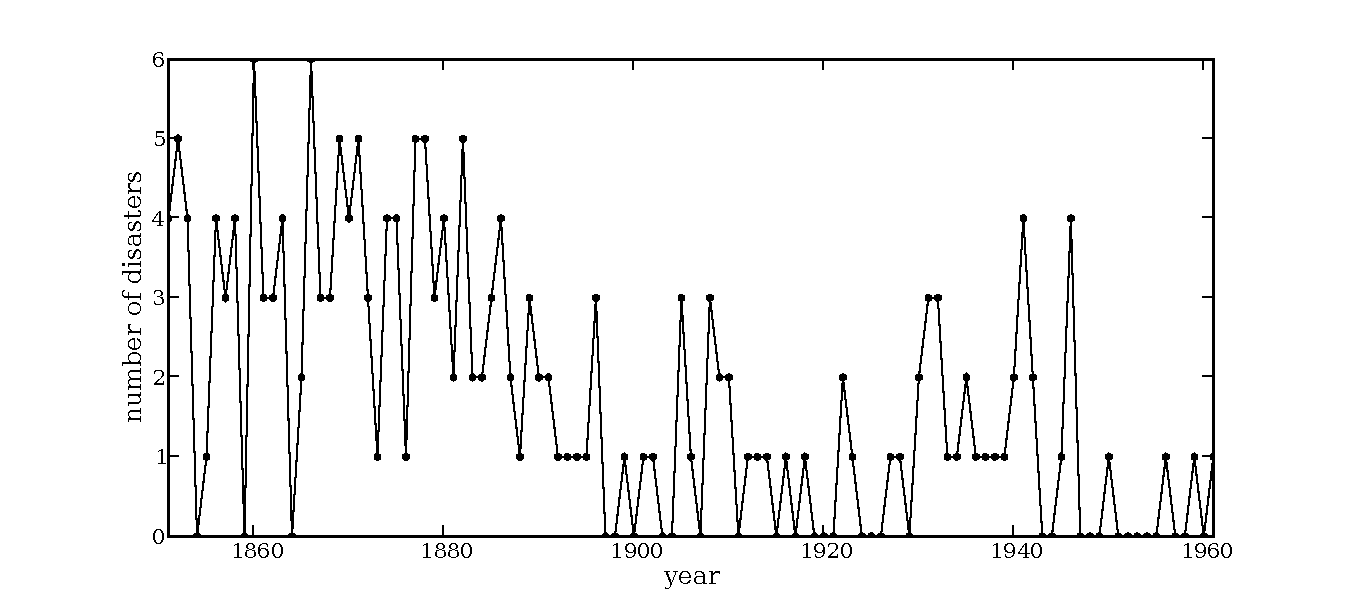
\epsfig{file=disasterts.pdf, width=15cm}
\caption{Recorded coal mining disasters in the UK. }
\label{fig:disaster-data}
\end{center}
\end{figure}
Occurrences of disasters in the series is thought to be derived from a Poisson process with a large rate parameter in the early part of the time series, and from one with a smaller rate in the later part. We are interested in locating the change point in the series, which perhaps is related to changes in mining safety regulations.

We represent our conceptual model formally as a statistical model:
\begin{equation}
    \begin{array}{ccc}
        (D_t | s, e, l) \sim \textup{Poisson}\left(r_t\right), & r_t=\left\{\begin{array}{lll}
            e &\textup{if}& t< s\\ l &\textup{if}& t\ge s
            \end{array}\right.,&t\in[t_l,t_h]\\
        s\sim \textup{Discrete Uniform}(t_l, t_h)\\
        e\sim \textup{Exponential}(r_e)\\
        l\sim \textup{Exponential}(r_l)
    \end{array}
    \label{disastermodel}
\end{equation}
The symbols are defined as:
\begin{description}
    \item[$D_t$:] The number of disasters in year $t$.
    \item[$r_t$:] The rate parameter of the Poisson distribution of disasters in year $t$.
    \item[$s$:] The year in which the rate parameter changes (the switchpoint).
    \item[$e$:] The rate parameter before the switchpoint $s$.
    \item[$l$:] The rate parameter after the switchpoint $s$.
    \item[$t_l$, $t_h$:] The lower and upper boundaries of year $t$.
    \item[$r_e$, $r_l$:] The rate parameters of the priors of the early and late rates, respectively.
    %\item[$\beta_e$, $\beta_l$:] Prior parameters (also called hyperparameters).
\end{description}
Because we have defined $D$ by its dependence on $s$, $e$ and $l$, the latter three are known as the `parents' of $D$ and $D$ is called their `child'. Similarly, the parents of $s$ are $t_l$ and $t_h$, and $s$ is the child of $t_l$ and $t_h$.


\subsection{Two types of variables}

At the model-specification stage (before the data are observed), $D$, $s$, $e$,
$r$ and $l$ are all random variables. Bayesian `random' variables have not
necessarily arisen from a physical random process. The Bayesian interpretation
of probability is \emph{epistemic}, meaning random variable $x$'s probability
distribution $p(x)$ represents our knowledge and uncertainty about $x$'s value
\citep{jaynes}. Candidate values of $x$ for which $p(x)$ is high are
relatively more probable, given what we know. Random variables are represented
in \pkg{PyMC} by the classes \code{Stochastic} and \code{Deterministic}.

The only \code{Deterministic} in the model is $r$. If we knew the values of
$r$'s parents ($s$, $l$ and $e$), we could compute the value of $r$ exactly. A
\code{Deterministic} like $r$ is defined by a mathematical function that returns
its value given values for its parents. \code{Deterministic} variables are
sometimes called the \emph{systemic} part of the model. The nomenclature is a
bit confusing, because these objects usually represent random variables; since
the parents of $r$ are random, $r$ is random also. A more descriptive (though
more awkward) name for this class would be \code{DeterminedByValuesOfParents}.

On the other hand, even if the values of the parents of variables $s$, $D$ (before observing the data), $e$ or $l$ were known, we would still be uncertain of their values. These variables are characterized by probability distributions that express how plausible their candidate values are, given values for their parents. The \code{Stochastic} class represents these variables. A more descriptive name for these objects might be \code{RandomEvenGivenValuesOfParents}.

We can represent model \ref{disastermodel} in a file called
\code{DisasterModel.py} (the actual file can be found in
\code{pymc/examples/}) as follows. First, we import the \pkg{PyMC} and \pkg{NumPy}
namespaces:
\begin{CodeInput}
from pymc import DiscreteUniform, Exponential, deterministic, Poisson, Uniform
import numpy
\end{CodeInput}
Notice that from \code{pymc} we have only imported a select few objects that are needed for this particular model, whereas the entire \code{numpy} namespace has been imported.

Next, we enter the actual data values into an array:
\begin{CodeInput}
disasters_array =   \
     numpy.array([ 4, 5, 4, 0, 1, 4, 3, 4, 0, 6, 3, 3, 4, 0, 2, 6,
                   3, 3, 5, 4, 5, 3, 1, 4, 4, 1, 5, 5, 3, 4, 2, 5,
                   2, 2, 3, 4, 2, 1, 3, 2, 2, 1, 1, 1, 1, 3, 0, 0,
                   1, 0, 1, 1, 0, 0, 3, 1, 0, 3, 2, 2, 0, 1, 1, 1,
                   0, 1, 0, 1, 0, 0, 0, 2, 1, 0, 0, 0, 1, 1, 0, 2,
                   3, 3, 1, 1, 2, 1, 1, 1, 1, 2, 4, 2, 0, 0, 1, 4,
                   0, 0, 0, 1, 0, 0, 0, 0, 0, 1, 0, 0, 1, 0, 1])
\end{CodeInput}
Note that you don't have to type in this entire array to follow along; the code is available in the source tree, in \code{pymc/examples/DisasterModel.py}.  Next, we create the switchpoint variable $s$:
\begin{CodeInput}
s = DiscreteUniform('s', lower=0, upper=110, doc='Switchpoint[year]')
\end{CodeInput}
\code{DiscreteUniform} is a subclass of \code{Stochastic} that represents uniformly-distributed discrete variables. Use of this distribution suggests that we have no preference \emph{a priori} regarding the location of the switchpoint; all values are equally likely. Now we create the exponentially-distributed variables $e$ and $l$ for the early and late Poisson rates, respectively:
\begin{CodeInput}
e = Exponential('e', beta=1)
l = Exponential('l', beta=1)
\end{CodeInput}
Next, we define the variable $r$, which selects the early rate $e$ for times before $s$ and the late rate $l$ for times after $s$. We create $r$ using the \code{deterministic} decorator, which converts the ordinary \proglang{Python} function $r$ into a \code{Deterministic} object.
\begin{CodeInput}
@deterministic(plot=False)
def r(s=s, e=e, l=l):
    """ Concatenate Poisson means """
    out = numpy.empty(len(disasters_array))
    out[:s] = e
    out[s:] = l
    return out
\end{CodeInput}
The last step is to define the number of disasters $D$. This is a stochastic variable, but unlike $s$, $e$ and $l$ we have observed its value. To express this, we set the argument \code{observed} to \code{True} (it is set to \code{False} by default). This tells \pkg{PyMC} that this object's value should not be changed:
\begin{CodeInput}
D = Poisson('D', mu=r, value=disasters_array, observed=True)
\end{CodeInput}

\subsection{Why are data and unknown variables represented by the same
object?}
Since it is represented by a \code{Stochastic} object, $D$ is defined by its dependence on its parent $r$ even though its value is fixed. This isn't just a quirk of \pkg{PyMC}'s syntax; Bayesian hierarchical notation itself makes no distinction between random variables and data. The reason is simple: to use Bayes' theorem to compute the posterior $p(e,s,l|D)$ of model (\ref{disastermodel}), we require the likelihood $p(D|e,s,l)$. Even though $D$'s value is known and fixed, we need to formally assign it a probability distribution as if it were a random variable. Remember, the likelihood and the probability function are essentially the same, except that the former is regarded as a function of the parameters and the latter as a function of the data.

This point can be counterintuitive at first, as many peoples' instinct is to regard data as fixed a priori and unknown variables as dependent on the data. One way to understand this is to think of statistical models like (\ref{disastermodel}) as predictive models for data, or as models of the processes that gave rise to data. Before observing the value of $D$, we could have sampled from its prior predictive distribution $p(D)$ (\emph{i.e.} the marginal distribution of the data) as follows:
\begin{enumerate}
    \item Sample $e$, $s$ and $l$ from their priors.
    \item Sample $D$ conditional on these values.
\end{enumerate}
Even after we observe the value of $D$, we need to use this process model to make inferences about $e$, $s$ and $l$ because its the only information we have about how the variables are related.

\subsection{Parents and children}

We have above created a \pkg{PyMC} probability model, which is simply a linked collection of variables. To see the nature of the links, import or run \code{DisasterModel.py} and examine $s$'s \code{parents} attribute from the \proglang{Python} prompt:
\begin{CodeInput}
>>> from pymc.examples import DisasterModel
>>> DisasterModel.s.parents
{`lower': 0, 'upper': 110}
\end{CodeInput}
The \code{parents} dictionary shows us the distributional parameters of $s$, which are constants. Now let's examinine $D$'s parents:
\begin{CodeInput}
>>> DisasterModel.D.parents
{`mu': <pymc.PyMCObjects.Deterministic 'r' at 0x3e51a70>}
\end{CodeInput}
We are using $r$ as a distributional parameter of $D$ (\emph{i.e.} $r$ is $D$'s parent). $D$ internally labels $r$ as \code{mu}, meaning $r$ plays the role of the rate parameter in $D$'s Poisson distribution. Now examine $r$'s \code{children} attribute:
\begin{CodeInput}
>>> DisasterModel.r.children
set([<pymc.distributions.Poisson 'D' at 0x3e51290>])
\end{CodeInput}
Because $D$ considers $r$ its parent, $r$ considers $D$ its child. Unlike \code{parents}, \code{children} is a set (an unordered collection of objects); variables do not associate their children with any particular distributional role. Try examining the \code{parents} and \code{children} attributes of the other parameters in the model.

A `directed acyclic graph' is a visualization of the parent-child relationships in the model. For example, in Figure~\ref{fig:dag-example} unobserved stochastic variables $s$, $e$ and $l$ are represented by open ellipses, observed stochastic variable $D$ is a filled ellipse and deterministic variable $r$ is a triangle. Arrows point from parent to child and display the label that the child assigns to the parent. See Section~\ref{graphical} for more details.
\begin{figure}[h!]
\begin{center}
   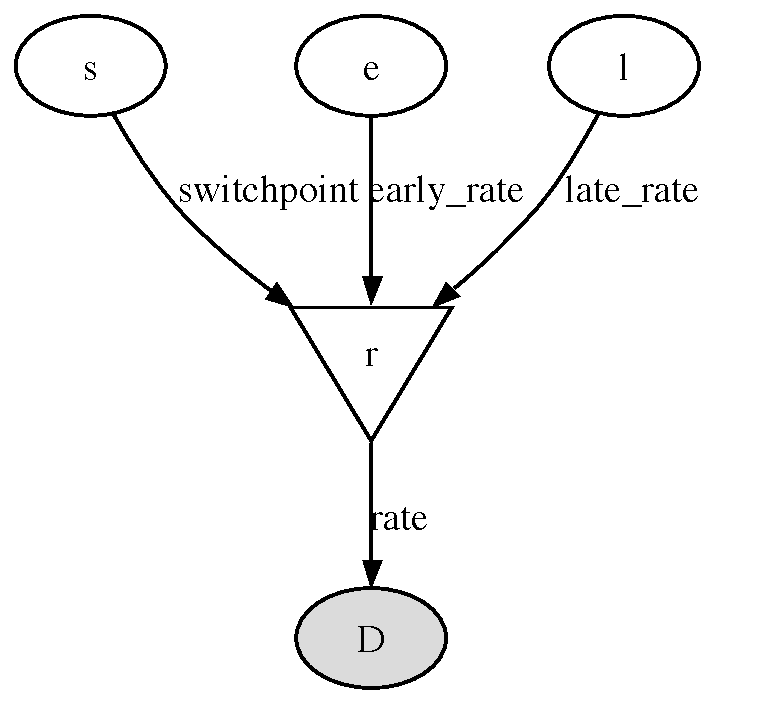
\epsfig{file=DisasterModel2.pdf, width=10cm}
   \caption{Directed acyclic graph of the relationships in the coal mining disaster model example.}
	\label{fig:dag-example}
\end{center}
\end{figure}

As the examples above have shown, \pkg{PyMC}  objects need to have a name 
assigned, such as \code{lower}, \code{upper} or \code{e}. These names 
are used for storage and post-processing:
\begin{itemize}
 \item as keys in on-disk databases,
 \item as node labels in model graphs,
 \item as axis labels in plots of traces, 
 \item as table~labels in summary statistics. 
\end{itemize}
A model instantiated with variables having identical names raises an
error to avoid name conflicts in the database storing the traces. In
general however, \pkg{PyMC}  uses references to the objects themselves, not 
their names, to identify variables. 



\subsection{Variables' values and log-probabilities}
All \pkg{PyMC} variables have an attribute called \code{value} that stores the current value of that variable. Try examining $D$'s value, and you'll see the initial value we provided for it:
\begin{CodeInput}
>>> DisasterModel.D.value
array([4, 5, 4, 0, 1, 4, 3, 4, 0, 6, 3, 3, 4, 0, 2, 6, 3, 3, 5, 4, 5, 3, 1,
      4, 4, 1, 5, 5, 3, 4, 2, 5, 2, 2, 3, 4, 2, 1, 3, 2, 2, 1, 1, 1, 1, 3,
      0, 0, 1, 0, 1, 1, 0, 0, 3, 1, 0, 3, 2, 2, 0, 1, 1, 1, 0, 1, 0, 1, 0,
      0, 0, 2, 1, 0, 0, 0, 1, 1, 0, 2, 3, 3, 1, 1, 2, 1, 1, 1, 1, 2, 4, 2,
      0, 0, 1, 4, 0, 0, 0, 1, 0, 0, 0, 0, 0, 1, 0, 0, 1, 0, 1])
\end{CodeInput}
If you check $e$'s, $s$'s and $l$'s values, you'll see random initial values generated by \pkg{PyMC}:
\begin{CodeInput}
>>> DisasterModel.s.value
44

>>> DisasterModel.e.value
0.33464706250079584

>>> DisasterModel.l.value
2.6491936762267811
\end{CodeInput}
Of course, since these are \code{Stochastic} elements, your values will be different than these. If you check $r$'s value, you'll see an array whose first $s$ elements are $e$ (here 0.33464706), and whose remaining elements are $l$ (here 2.64919368):
\begin{CodeInput}
>>> DisasterModel.r.value
array([ 0.33464706,  0.33464706,  0.33464706,  0.33464706,  0.33464706,
       0.33464706,  0.33464706,  0.33464706,  0.33464706,  0.33464706,
       0.33464706,  0.33464706,  0.33464706,  0.33464706,  0.33464706,
       0.33464706,  0.33464706,  0.33464706,  0.33464706,  0.33464706,
       0.33464706,  0.33464706,  0.33464706,  0.33464706,  0.33464706,
       0.33464706,  0.33464706,  0.33464706,  0.33464706,  0.33464706,
       0.33464706,  0.33464706,  0.33464706,  0.33464706,  0.33464706,
       0.33464706,  0.33464706,  0.33464706,  0.33464706,  0.33464706,
       0.33464706,  0.33464706,  0.33464706,  0.33464706,  2.64919368,
       2.64919368,  2.64919368,  2.64919368,  2.64919368,  2.64919368,
       2.64919368,  2.64919368,  2.64919368,  2.64919368,  2.64919368,
       2.64919368,  2.64919368,  2.64919368,  2.64919368,  2.64919368,
       2.64919368,  2.64919368,  2.64919368,  2.64919368,  2.64919368,
       2.64919368,  2.64919368,  2.64919368,  2.64919368,  2.64919368,
       2.64919368,  2.64919368,  2.64919368,  2.64919368,  2.64919368,
       2.64919368,  2.64919368,  2.64919368,  2.64919368,  2.64919368,
       2.64919368,  2.64919368,  2.64919368,  2.64919368,  2.64919368,
       2.64919368,  2.64919368,  2.64919368,  2.64919368,  2.64919368,
       2.64919368,  2.64919368,  2.64919368,  2.64919368,  2.64919368,
       2.64919368,  2.64919368,  2.64919368,  2.64919368,  2.64919368,
       2.64919368,  2.64919368,  2.64919368,  2.64919368,  2.64919368,
       2.64919368,  2.64919368,  2.64919368,  2.64919368,  2.64919368])
\end{CodeInput}
To compute its value, $r$ calls the funtion we used to create it, passing in the values of its parents.

\code{Stochastic} objects can evaluate their probability mass or density functions at their current values given the values of their parents. The logarithm of a stochastic object's probability mass or density can be accessed via the \code{logp} attribute. For vector-valued variables like $D$, the \code{logp} attribute returns the sum of the logarithms of the joint probability or density of all elements of the value. Try examining $s$'s and $D$'s log-probabilities and $e$'s and $l$'s log-densities:
\begin{CodeInput}
>>> DisasterModel.s.logp
-4.7095302013123339

>>> DisasterModel.D.logp
-1080.5149888046033

>>> DisasterModel.e.logp
-0.33464706250079584

>>> DisasterModel.l.logp
-2.6491936762267811
\end{CodeInput}
\code{Stochastic} objects need to call an internal function to compute their \code{logp} attributes, as $r$ needed to call an internal function to compute its value. Just as we created $r$ by decorating a function that computes its value, it's possible to create custom \code{Stochastic} objects by decorating functions that compute their log-probabilities or densities (see Section~\ref{chap:modelbuilding}). Users are thus not limited to the set of of statistical distributions provided by \pkg{PyMC}.

\subsection{Using variables as parents of other variables}

Let's take a closer look at our definition of $r$:
\begin{CodeInput}
@deterministic(plot=False)
def r(s=s, e=e, l=l):
    """ Concatenate Poisson means """
    out = numpy.empty(len(disasters_array))
    out[:s] = e
    out[s:] = l
    return out
\end{CodeInput}
The arguments $s$, $e$ and $l$ are \code{Stochastic} objects, not numbers. Why aren't errors raised when we attempt to slice array \code{out} up to a \code{Stochastic} object?

Whenever a variable is used as a parent for a child variable, \pkg{PyMC} replaces it with its \code{value} attribute when the child's value or log-probability is computed. When $r$'s value is recomputed, \code{s.value} is passed to the function as argument \code{s}. To see the values of the parents of $r$ all together, look at \code{r.parents.value}.

\subsection{Fitting the model with MCMC}

\pkg{PyMC} provides several objects that fit probability models (linked collections of variables) like ours. The primary such object, \code{MCMC}, fits models with a Markov chain Monte Carlo algorithm \citep{Gamerman:1997tb}. To create an \code{MCMC} object to handle our model, import \code{DisasterModel.py} and use it as an argument for \code{MCMC}:
\begin{CodeInput}
>>> from pymc.examples import DisasterModel
>>> from pymc import MCMC
>>> M = MCMC(DisasterModel)
\end{CodeInput}
In this case \code{M} will expose variables \code{s}, \code{e}, \code{l}, \code{r} and \code{D} as attributes; that is, \code{M.s} will be the same object as \code{DisasterModel.s}.

To run the sampler, call the MCMC object's \code{sample()} (or \code{isample()}, for  interactive sampling) method with arguments for the number of iterations, burn-in length, and thinning interval (if desired):
\begin{CodeInput}
>>> M.isample(iter=10000, burn=1000, thin=10)
\end{CodeInput}
After a few seconds, you should see that sampling has finished normally. The model has been fitted.

\subsection{What does it mean to fit a model?}

`Fitting' a model means characterizing its posterior distribution, by whatever suitable means. In this case, we are trying to represent the posterior $p(s,e,l|D)$ by a set of joint samples from it. To produce these samples, the MCMC sampler randomly updates the values of $s$, $e$ and $l$ according to the Metropolis-Hastings algorithm (\citet{gelman}) for \code{iter}  iterations.

As the number of samples tends to infinity, the MCMC distribution of $s$, $e$
and $l$ converges to the stationary distribution. In other words, their
values can be considered as random draws from the posterior $p(s,e,l|D)$.
\pkg{PyMC} assumes that the \code{burn} parameter specifies a `sufficiently large'
number of iterations for convergence of the algorithm, so it is up to the user
to verify
that this is the case (see Section~\ref{chap:modelchecking}). Consecutive values
sampled from $s$, $e$ and $l$ are necessarily dependent on the previous sample,
since it is a Markov chain. However, MCMC often results in strong
autocorrelation among samples that can result in imprecise posterior inference.
To circumvent this, it is often effective to thin the sample by only retaining
every $k$th sample, where $k$ is an integer value. This thinning interval is
passed to the sampler via the \code{thin} argument.

If you are not sure ahead of time what values to choose for the \code{burn} and \code{thin} parameters, you may want to retain all the MCMC samples, that is to set \code{burn=0} and \code{thin=1} (these are the default values for the samplers provided by \pkg{PyMC}), and then discard the `burnin period' and thin the samples after examining the traces (the series of samples). See \citet{gelman} for general guidance.

\subsection{Accessing the samples}
The output of the MCMC algorithm is a `trace', the sequence of retained
samples for each variable in the model. These traces can be accessed
using the \code{trace(name, chain=-1)} method. For example:
\begin{CodeInput}
>>> M.trace('s')[:]
array([41, 40, 40, ..., 43, 44, 44])
\end{CodeInput}
The trace slice \code{[start:stop:step]} works just like the \pkg{NumPy} array
slice. By default, the returned trace array contains the samples from the
last call to \code{sample}, that is, \code{chain=-1}, but the trace from
previous sampling runs can be retrieved by specifying the correspondent
chain index. To return the trace from all chains, simply use
\code{chain=None}. \footnote{Note that the unknown variables $s$, $e$, $l$ and $r$ will all
accrue samples, but $D$ will not because its value has been observed and is
not updated. Hence $D$ has no trace and calling \code{M.trace('D')[:]} will
raise an error. }

% Alternatively, the trace may be retrieved directly from the variable:
% \begin{CodeInput}
%   >>> s.trace()
%   array([41, 40, 40, ..., 43, 44, 44])
% \end{CodeInput}

\subsection{Sampling output}
You can examine the marginal posterior of any variable by plotting a histogram of its trace:
\begin{CodeInput}
>>> from pylab import hist, show
>>> hist(M.trace('l')[:])
(array([   8,   52,  565, 1624, 2563, 2105, 1292,  488,  258,   45]),
array([ 0.52721865,  0.60788251,  0.68854637,  0.76921023,  0.84987409,
       0.93053795,  1.01120181,  1.09186567,  1.17252953,  1.25319339]),
<a list of 10 Patch objects>)
>>> show()
\end{CodeInput}
You should see something similar to Figure~\ref{fig:hist}.
\begin{figure}[ht!]
\begin{center}
   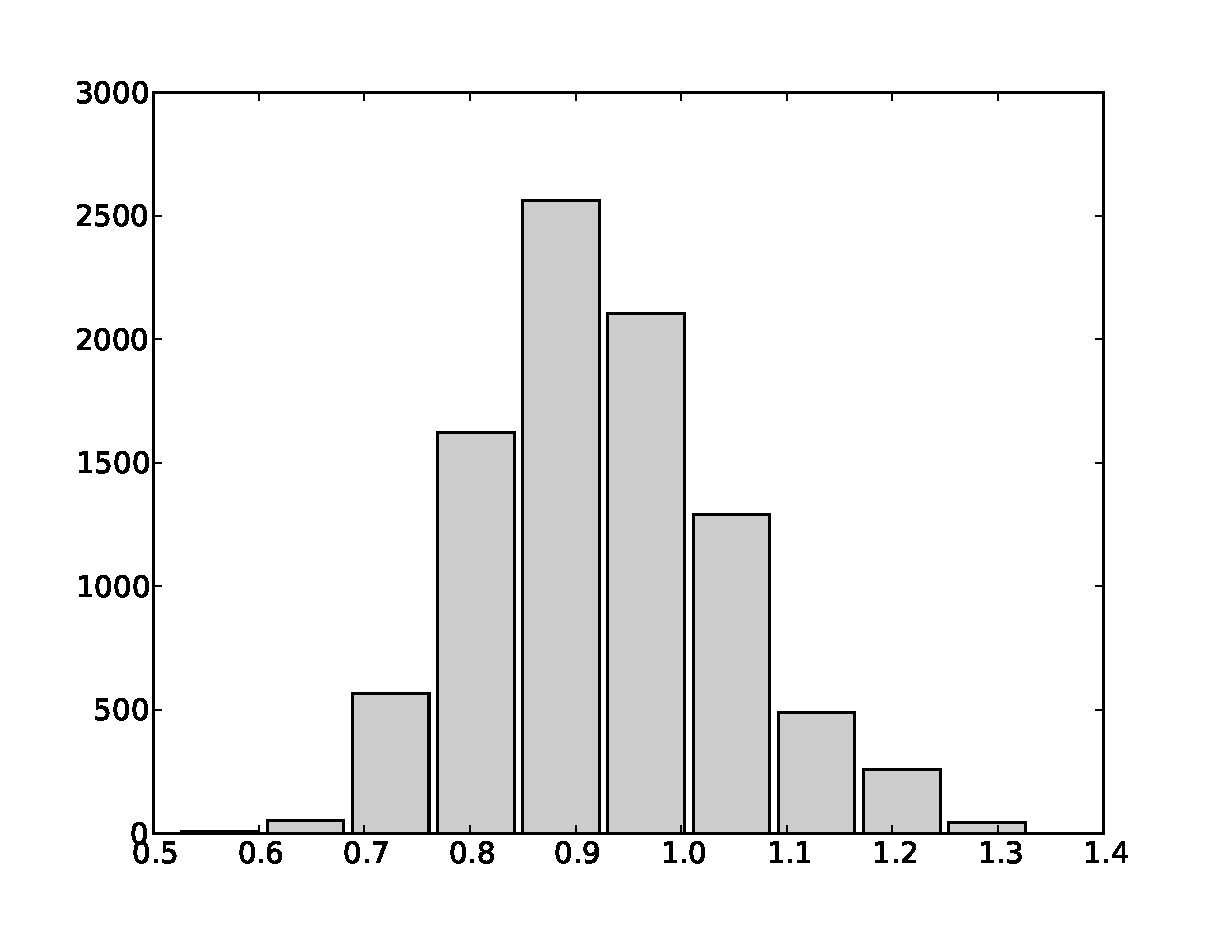
\epsfig{file=ltrace.pdf, width=12cm}
   \caption{Histogram of the marginal posterior probability of parameter $l$.}
	\label{fig:hist}
\end{center}
\end{figure}

\pkg{PyMC} has its own plotting functionality, via the optional
\code{matplotlib} module as noted in the installation notes. The
\code{Matplot} module includes a \code{plot} function that takes the
model (or a single parameter) as an argument:
\begin{CodeInput}
>>> from pymc.Matplot import plot
>>> plot(M)
\end{CodeInput}
For each variable in the model, \code{plot} generates a composite figure, such as that for the switchpoint in the disasters model (Figure~\ref{fig:switch}). The left-hand pane of this figure~shows the temporal series of the samples from $s$, while the right-hand pane shows a histogram of the trace. The trace is useful for evaluating and diagnosing the algorithm's performance (see \cite*{gelman}), while the histogram is useful for visualizing the posterior.
\begin{figure}[h!]
\begin{center}
   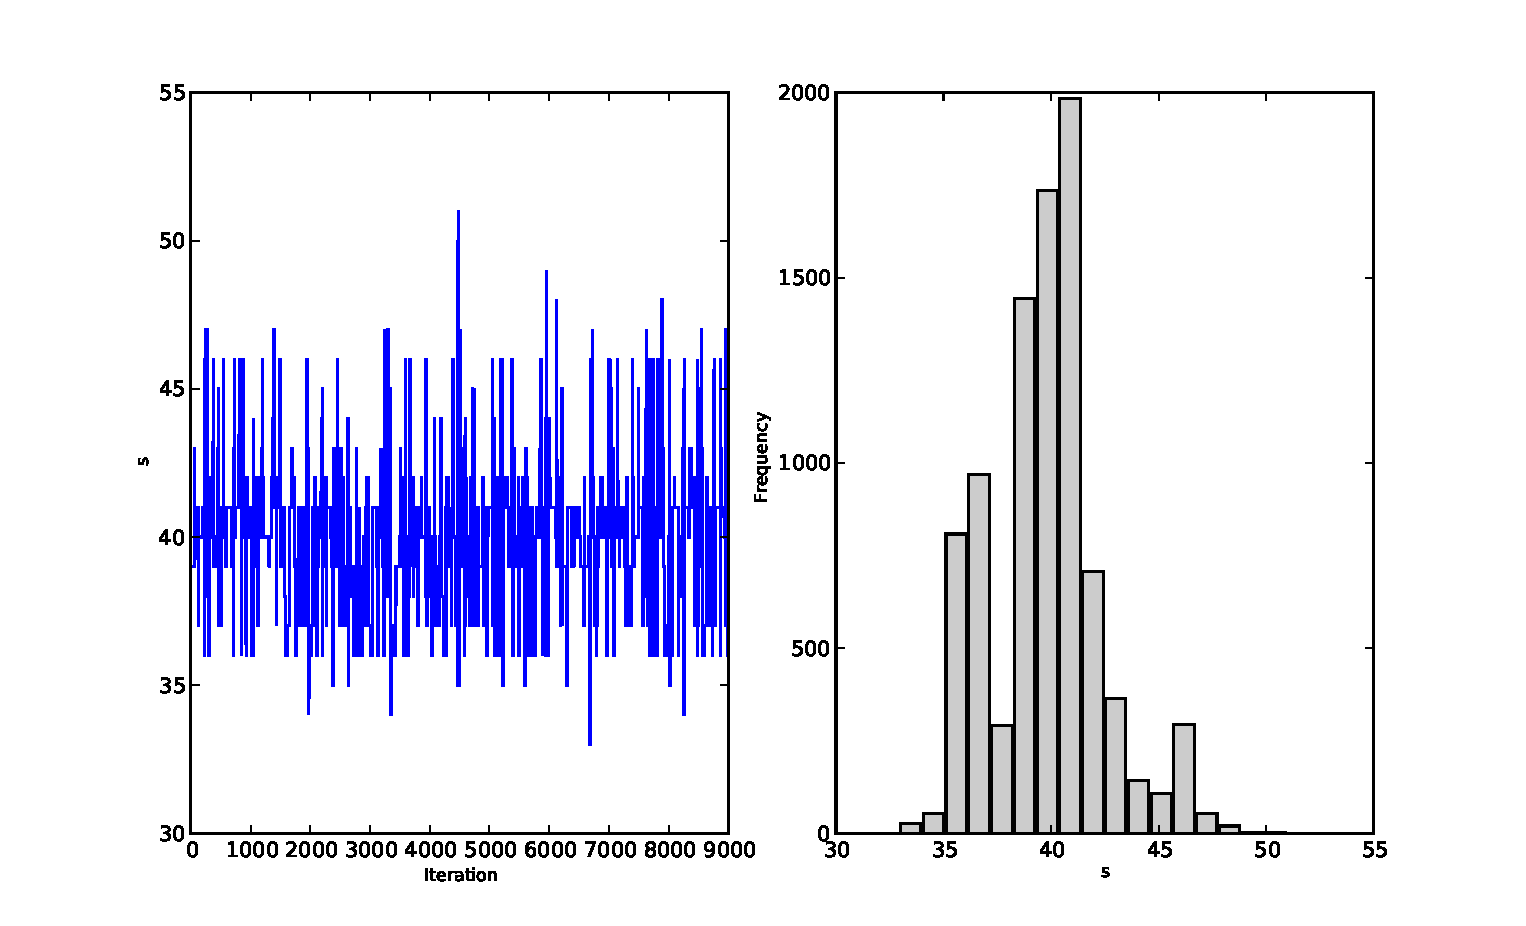
\epsfig{file=spost.pdf, width=15cm}
   \caption{Temporal series and histogram of the samples drawn for $s$. }
\label{fig:switch}
\end{center}
\end{figure}

For a non-graphical summary of the posterior, simply call \code{M.stats()}.


\subsection{Imputation of Missing Data}

%\label{subsec:missing_data}

As with most ``textbook examples", the models we have examined so far assume that the associated data are complete. That is, there are no missing values corresponding to any observations in the dataset. However, many real-world datasets contain one or more missing values, usually due to some logistical problem during the data collection process. The easiest way of dealing with observations that contain missing values is simply to exclude them from the analysis. However, this results in loss of information if an excluded observation contains valid values for other quantities, and can bias results. An alternative is to impute the missing values, based on information in the rest of the model.

For example, consider a survey dataset for some wildlife species:

\begin{table}[h!]
\begin{center}
\begin{tabular}{cccc}
\hline
Count & Site & Observer & Temperature\\
\hline
15 & 1 & 1 & 15\\
10 & 1 & 2 & NA\\
6 & 1 & 1 & 11\\
\hline
\end{tabular}
\end{center}
\end{table}

Each row contains the number of individuals seen during the survey, along with three covariates: the site on which the survey was conducted, the observer that collected the data, and the temperature during the survey. If we are interested in modelling, say, population size as a function of the count and the associated covariates, it is difficult to accommodate the second observation because the temperature is missing (perhaps the thermometer was broken that day). Ignoring this observation will allow us to fit the model, but it wastes information that is contained in the other covariates.

In a Bayesian modelling framework, missing data are accommodated simply by treating them as unknown model parameters. Values for the missing data $\tilde{y}$ are estimated naturally, using the posterior predictive distribution:

\begin{equation}
  p(\tilde{y}|y) = \int p(\tilde{y}|\theta) f(\theta|y) d\theta
\end{equation}

This describes additional data $\tilde{y}$, which may either be considered unobserved data or potential future observations. We can use the posterior predictive distribution to model the likely values of missing data, which accounts for both predictive and inferential uncertainty.

Consider the coal mining disasters data introduced previously. Assume that two years of data are missing from the time series; we indicate this in the data array by the use of an arbitrary placeholder value, \code{None}.

\begin{CodeInput}
x = numpy.array([ 4, 5, 4, 0, 1, 4, 3, 4, 0, 6, 3, 3, 4, 0, 2, 6,
3, 3, 5, 4, 5, 3, 1, 4, 4, 1, 5, 5, 3, 4, 2, 5,
2, 2, 3, 4, 2, 1, 3, None, 2, 1, 1, 1, 1, 3, 0, 0,
1, 0, 1, 1, 0, 0, 3, 1, 0, 3, 2, 2, 0, 1, 1, 1,
0, 1, 0, 1, 0, 0, 0, 2, 1, 0, 0, 0, 1, 1, 0, 2,
3, 3, 1, None, 2, 1, 1, 1, 1, 2, 4, 2, 0, 0, 1, 4,
0, 0, 0, 1, 0, 0, 0, 0, 0, 1, 0, 0, 1, 0, 1])
\end{CodeInput}

To estimate these values in \pkg{PyMC}, we generate a masked array. These are specialised \pkg{NumPy} arrays that contain a matching \code{True} or \code{False} value for each element to indicate if that value should be excluded from any computation. Masked arrays can be generated using \pkg{NumPy}'s \code{ma.masked_equal} function:
\begin{CodeInput}
>>> masked_data = numpy.ma.masked_equal(x, value=None)
>>> masked_data
masked_array(data = [4 5 4 0 1 4 3 4 0 6 3 3 4 0 2 6 3 3 5 4 5 3 1 4 4 1 5 5 3
 4 2 5 2 2 3 4 2 1 3 -- 2 1 1 1 1 3 0 0 1 0 1 1 0 0 3 1 0 3 2 2 0 1 1 1 0 1 0
 1 0 0 0 2 1 0 0 0 1 1 0 2 3 3 1 -- 2 1 1 1 1 2 4 2 0 0 1 4 0 0 0 1 0 0 0 0 0 1
 0 0 1 0 1],
 mask = [False False False False False False False False False False False False
 False False False False False False False False False False False False
 False False False False False False False False False False False False
 False False False  True False False False False False False False False
 False False False False False False False False False False False False
 False False False False False False False False False False False False
 False False False False False False False False False False False  True
 False False False False False False False False False False False False
 False False False False False False False False False False False False
 False False False],
  fill_value=?)

\end{CodeInput}

This masked array, in turn, can then be passed to \pkg{PyMC}'s own \code{Impute} function, which replaces the missing values with Stochastic variables of the desired type. For the coal mining disasters problem, recall that disaster events were modelled as Poisson variates:

\begin{CodeInput}
>>> from pymc import Impute
>>> D = Impute('D', Poisson, masked_data, mu=r)
>>> D
[<pymc.distributions.Poisson 'D[0]' at 0x4ba42d0>,
 <pymc.distributions.Poisson 'D[1]' at 0x4ba4330>,
 <pymc.distributions.Poisson 'D[2]' at 0x4ba44d0>,
 <pymc.distributions.Poisson 'D[3]' at 0x4ba45f0>,
...
 <pymc.distributions.Poisson 'D[110]' at 0x4ba46d0>]
\end{CodeInput}

Here $r$ is an array of means for each year of data, allocated according to the location of the switchpoint. Each element in $D$ is a Poisson Stochastic, irrespective of whether the observation was missing or not. The difference is that actual observations are data Stochastics (\code{observed=True}), while the missing values are non-data Stochastics. The latter are considered unknown, rather than fixed, and therefore estimated by the MCMC algorithm, just as unknown model parameters.

In this example, we have manually generated the masked array for illustration. In practice, the \code{Impute} function will mask arrays automatically, replacing all \code{None} values with Stochastics. Hence, only the original data array needs to be passed.

The entire model looks very similar to the original model:

\begin{CodeInput}
s = DiscreteUniform('s', lower=0, upper=110)
e = Exponential('e', beta=1)
l = Exponential('l', beta=1)

@deterministic(plot=False)
def r(s=s, e=e, l=l):
    """Allocate appropriate mean to time series"""
    out = numpy.empty(len(disasters_array))
    out[:s] = e
    out[s:] = l
    return out

D = Impute('D', Poisson, x, mu=r)
\end{CodeInput}

\begin{figure}[ht]
\begin{center}
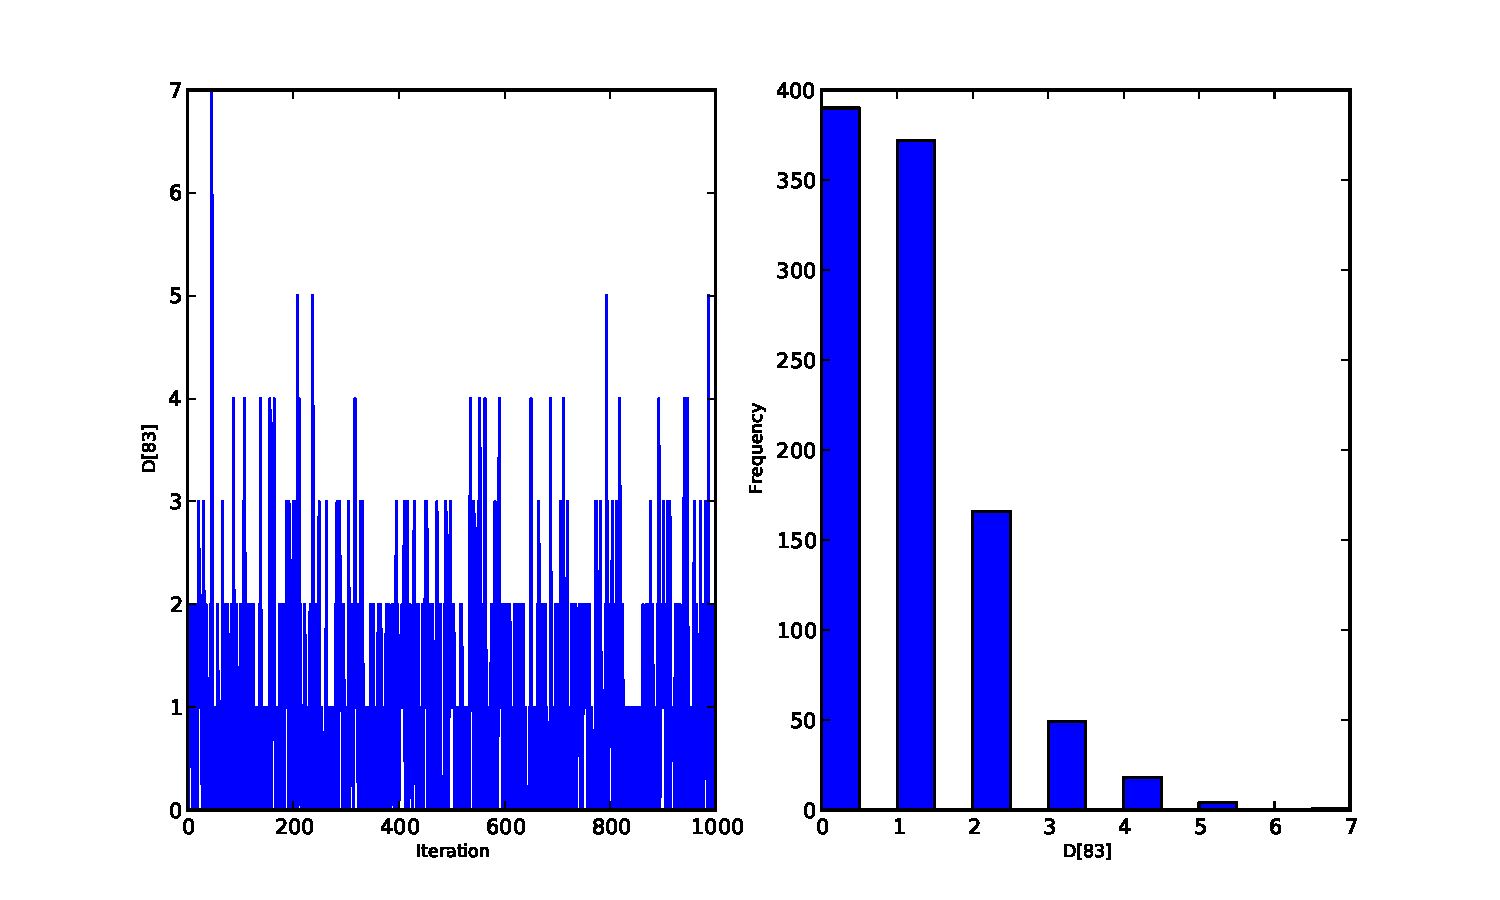
\includegraphics[width=15cm]{missing.pdf}
\caption{Trace and posterior distribution of the second missing data point in the example.}
\label{fig:missing}
\end{center}
\end{figure}


The main limitation of this approach for imputation is performance. Because each
element in the data array is modelled by an individual Stochastic, rather than a
single Stochastic for the entire array, the number of nodes in the overall model
increases from 4 to 113. This significantly slows the rate of sampling, due to
the overhead costs associated with iterations over individual nodes.


\subsection{Fine-tuning the MCMC algorithm}

MCMC objects handle individual variables via \emph{step methods}, which determine how parameters are updated at each step of the MCMC algorithm. By default, step methods are automatically assigned to variables by \pkg{PyMC}. To see which step methods $M$ is using, look at its \code{step_method_dict} attribute with respect to each parameter:
\begin{CodeInput}
>>> M.step_method_dict[DisasterModel.s]
[<pymc.StepMethods.DiscreteMetropolis object at 0x3e8cb50>]

>>> M.step_method_dict[DisasterModel.e]
[<pymc.StepMethods.Metropolis object at 0x3e8cbb0>]

>>> M.step_method_dict[DisasterModel.l]
[<pymc.StepMethods.Metropolis object at 0x3e8ccb0>]
\end{CodeInput}
The value of \code{step_method_dict} corresponding to a particular variable is a list of the step methods $M$ is using to handle that variable.

You can force $M$ to use a particular step method by calling \code{M.use_step_method} before telling it to sample. The following call will cause $M$ to handle $l$ with a standard \code{Metropolis} step method, but with proposal standard deviation equal to $2$:
\begin{CodeInput}
>>> from pymc import Metropolis
M.use_step_method(Metropolis, DisasterModel.l, proposal_sd=2.)
\end{CodeInput}

Another step method class, \code{AdaptiveMetropolis}, is better at handling highly-correlated variables. If your model mixes poorly, using \code{AdaptiveMetropolis} is a sensible first thing to try.



\subsection{Beyond the basics}
That was a brief introduction to basic \pkg{PyMC} usage. Many more topics are covered in the subsequent sections, including:
\begin{itemize}
   \item Class \code{Potential}, another building block for probability models in addition to \code{Stochastic} and \code{Deterministic}
   \item Normal approximations
   \item Using custom probability distributions
   \item Object architecture
   \item Saving traces to the disk, or streaming them to the disk during sampling
   \item Writing your own step methods and fitting algorithms.
\end{itemize}
Also, be sure to check out the documentation for the Gaussian process extension,
which is available on \pkg{PyMC}'s
download page at \href{http://code.google.com/p/pymc/downloads/list}{http://code.google.com/p/pymc/downloads/list}.



\section{Building models}
\label{chap:modelbuilding}

Bayesian inference begins with specification of a probability model relating unknown variables to data. \pkg{PyMC} provides three basic building blocks for probability models: \code{Stochastic}, \code{Deterministic} and \code{Potential}.

A \code{Stochastic} object represents a variable whose value is not completely determined by its parents, and a \code{Deterministic} object represents a variable that is entirely determined by its parents. \code{Stochastic} and \code{Deterministic} are subclasses of the \code{Variable} class, which only serves as a template for other classes and is never actually implemented in models.

The third basic class, \code{Potential}, represents `factor potentials' \citep{dawidmarkov,Jordan:2004p5439}, which are \emph{not} variables but simply terms and/or constraints that are multiplied into joint distributions to modify them. \code{Potential} and \code{Variable} are subclasses of \code{Node}.

\medskip
\pkg{PyMC} probability models are simply linked groups of \code{Stochastic}, \code{Deterministic} and \code{Potential} objects. These objects have very limited awareness of the models in which they are embedded and do not themselves possess methods for updating their values in fitting algorithms. Objects responsible for fitting probability models are described in Section~\ref{chap:modelfitting}.



\subsection[The Stochastic class]{The \code{Stochastic} class}
\label{stochastic}


A stochastic variable has the following primary attributes:
\begin{description}
    \item[\code{value}:] The variable's current value.
    \item[\code{logp}:] The log-probability of the variable's current value given the values of its parents.
\end{description}
A stochastic variable can optionally be endowed with a method called \code{\bfseries rand}, which draws a value for the variable given the values of its parents\footnote{Note that the \code{random} method does not provide a Gibbs sample unless the variable has no children.}. Stochastic variables have the following additional attributes:
\begin{description}
    \item[\code{parents}:] A dictionary containing the variable's parents. The keys of the dictionary are to the labels assigned to the parents by the variable, and the values correspond to the actual parents. For example, the keys of $s$'s parents dictionary in model (\ref{disastermodel}) would be \code{`t_l'} and \code{`t_h'}. The actual parents (\emph{i.e.} the values of the dictionary) may be of any class or type.
    \item[\code{children}:] A set containing the variable's children.
    \item[\code{extended_parents}:] A set containing all stochastic variables on which the variable depends, either directly or via a sequence of deterministic variables. If the value of any of these variables changes, the variable will need to recompute its log-probability.
    \item[\code{extended_children}:] A set containing all stochastic variables and potentials that depend on the variable, either directly or via a sequence of deterministic variables. If the variable's value changes, all of these variables and potentials will need to recompute their log-probabilities.
    % \item[\code{coparents}:] A set containing all the stochastic variables that share extended children with the variable.
    % \item[\code{moral_neighbors}:] A set containing the union of the variable's extended parents, extended children and coparents, with Potential objects removed.
    % \item[\code{markov_blanket}:] A set containing self and self's moral neighbors.
    \item[\code{observed}:] A flag (boolean) indicating whether the variable's value has been observed (is fixed).
    \item[\code{dtype}:] A \pkg{NumPy} dtype object (such as \code{numpy.int}) that specifies the type of the variable's value. The variable's value is always cast to this type. If this is \code{None} (default) then no type is enforced.
    % \item[\code{__name__}:] The name of the variable, should be unique.
    %    \item[\code{__doc__}:] The docstring of the variable.
\end{description}

\subsection{Creation of stochastic variables}
There are three main ways to create stochastic variables, called the \textbf{automatic}, \textbf{decorator}, and \textbf{direct} interfaces.

\begin{description}
    \item[Automatic] Stochastic variables with standard distributions provided by \pkg{PyMC} (see Appendices A-D) can be created in a single line using special subclasses of \code{Stochastic}. For example, the uniformly-distributed discrete variable $s$ in (\ref{disastermodel}) could be created using the automatic interface as follows:
\begin{CodeInput}
import pymc as pm
s = pm.DiscreteUniform('s', 1851, 1962, value=1900)
\end{CodeInput}

    In addition to the classes in the appendix, \code{scipy.stats.distributions}' random variable classes are wrapped as \code{Stochastic} subclasses if \pkg{SciPy} is installed. These distributions are in the submodule \code{pymc.\pkg{SciPy}Distributions}.

    Users can call the class factory \code{stochastic_from_dist} to produce \code{Stochastic} subclasses of their own from probability distributions not included with \pkg{PyMC}.%  These classes' init methods take the following arguments:
    % \begin{description}
    %     \item[\code{name}:] The name of the variable.
    %     \item[\code{value}:] An initial value for the variable.
    %     \item[\code{parents}:] Keyword arguments specifying the parents of the variable.
    %     \item[\code{observed} (optional)]
    %     \item[\code{doc} (optional):] The docstring of the variable.
    %     \item[\code{verbose} (optional):] An integer from 0 to 3.
    %     \item[\code{trace} (optional):] A boolean indicating whether a trace should be kept for this variable in Monte Carlo fitting methods.
    %     \item[\code{cache_depth}:] See Section~\ref{sec:caching}.
    % \end{description}


    \item[Decorator] Uniformly-distributed discrete stochastic variable $s$ in (\ref{disastermodel}) could alternatively be created from a function that computes its log-probability as follows:
\begin{CodeInput}
@pm.stochastic(dtype=int)
def s(value=1900, t_l=1851, t_h=1962):
"""The switchpoint for the rate of disaster occurrence."""
if value > t_h or value < t_l:
    return -numpy.inf
else:
    return -numpy.log(t_h - t_l + 1)
\end{CodeInput}
Note that this is a simple \proglang{Python} function preceded by a \proglang{Python} expression called a decorator \citep{python}, here called \code{@stochastic}. Generally, decorators enhance functions with additional properties or functionality. The \code{Stochastic} object produced by the \code{@stochastic} decorator will evaluate its log-probability using the function $s$. The \code{value} argument, which is required, provides an initial value for the variable. The remaining arguments will be assigned as parents of $s$ (\emph{i.e.} they will populate the \code{parents} dictionary).

To emphasize, the \proglang{Python} function decorated by \code{@stochastic} should compute the \emph{log}-density or \emph{log}-probability of the variable. That's why the return value in the example above is $-\log(t_h-t_l+1)$ rather than $1/(t_h-t_l+1)$.

The \code{value} and parents of stochastic variables may be any objects, provided the log-probability function returns a real number (\code{float}). \pkg{PyMC} and \pkg{SciPy} both provide implementations of several standard probability distributions that may be helpful for creating custom stochastic variables. Based on informal comparison using version 2.0, the distributions in \pkg{PyMC} tend to be approximately an order of magnitude faster than their counterparts in \pkg{SciPy} (using version 0.7). See the \pkg{PyMC} wiki page on benchmarks at \href{http://code.google.com/p/pymc/wiki/Benchmarks}{http://code.google.com/p/pymc/wiki/Benchmarks}.

    The decorator \code{stochastic} can take any of the arguments \code{Stochastic.__init__} takes except \code{parents}, \code{logp}, \code{random}, \code{doc} and \code{value}. These arguments include \code{trace}, \code{plot}, \code{verbose}, \code{dtype}, \code{rseed} and \code{name}.

    The decorator interface has a slightly more complex implementation which allows you to specify a \code{random} method for sampling the stochastic variable's value conditional on its parents.
    \begin{CodeInput}
@pm.stochastic(dtype=int)
def s(value=1900, t_l=1851, t_h=1962):
"""The switchpoint for the rate of disaster occurrence."""

def logp(value, t_l, t_h):
    if value > t_h or value < t_l:
        return -numpy.inf
    else:
        return -numpy.log(t_h - t_l + 1)

def random(t_l, t_h):
    return numpy.round( (t_l - t_h) * random() ) + t_l

\end{CodeInput}
The stochastic variable again gets its name, docstring and parents from function $s$, but in this case it will evaluate its log-probability using the \code{logp} function. The \code{random} function will be used when \code{s.random()} is called. Note that \code{random} doesn't take a \code{value} argument, as it generates values itself.

    \item[Direct] It's possible to instantiate \code{Stochastic} directly:
\begin{CodeInput}
def s_logp(value, t_l, t_h):
if value > t_h or value < t_l:
    return -numpy.inf
else:
    return -numpy.log(t_h - t_l + 1)

def s_rand(t_l, t_h):
return numpy.round( (t_l - t_h) * random() ) + t_l

s = pm.Stochastic( logp = s_logp,
            doc = 'The switchpoint for the rate of disaster occurrence.',
            name = 's',
            parents = {`t_l': 1851, 't_h': 1962},
            random = s_rand,
            trace = True,
            value = 1900,
            dtype=int,
            rseed = 1.,
            observed = False,
            cache_depth = 2,
            plot=True,
            verbose = 0)
\end{CodeInput}
Notice that the log-probability and random variate functions are specified externally and passed to \code{Stochastic} as arguments. This is a rather awkward way to instantiate a stochastic variable; consequently, such implementations should be rare.

\end{description}

\subsection{A warning: Don't update stochastic variables' values in-place}


\code{Stochastic} objects' values should not be updated in-place. This confuses \pkg{PyMC}'s caching scheme and corrupts the process used for accepting or rejecting proposed values in the MCMC algorithm. The only way a stochastic variable's value should be updated is using statements of the following form:
\begin{CodeInput}
A.value = new_value
\end{CodeInput}
The following are in-place updates and should \emph{never} be used:
\begin{itemize}
    \item \code{A.value += 3}
    \item \code{A.value[2,1] = 5}
    \item \code{A.value.attribute = new_attribute_value}.
\end{itemize}

This restriction becomes onerous if a step method proposes values for the elements of an array-valued variable separately. In this case, it may be preferable to partition the variable into several scalar-valued variables stored in an array or list.


\subsection{Data} \label{data}


Data are represented by \code{Stochastic} objects whose \code{observed} attribute is set to \code{True}. Although the data are modelled with statistical distributions, their values should be treated as immutable~(since they have been observed). If a stochastic variable's \code{observed} flag is \code{True}, its value cannot be changed, and it won't be sampled by the fitting method.

\subsection{Declaring stochastic variables to be data}

In each interface, an optional keyword argument \code{observed} can be set to \code{True}. In the decorator interface, this argument is added to the \code{@stochastic} decorator:

\begin{CodeInput}
@pm.stochastic(observed=True)
\end{CodeInput}

In the other interfaces, the \code{observed=True} argument is added to the initialization arguments:

\begin{CodeInput}
x = pm.Binomial('x', value=7, n=10, p=.8, observed=True)
\end{CodeInput}

Alternatively, in the decorator interface only, a \code{Stochastic} object's \code{observed} flag can be set to true by using an \code{@observed} decorator in place of the \code{@stochastic} decorator:
\begin{CodeInput}
@observed(dtype=int)
    def ...
\end{CodeInput}


\subsection[The Deterministic class]{The \code{Deterministic} class}
\label{deterministic}


The \code{Deterministic} class represents variables whose values are completely determined by the values of their parents. For example, in model (\ref{disastermodel}), $r$ is a \code{deterministic} variable. Recall it was defined by
\begin{eqnarray*}
    r_t=\left\{\begin{array}{ll}
        e & t\le s\\ l & t>s
        \end{array}\right.,
\end{eqnarray*}
so $r$'s value can be computed exactly from the values of its parents $e$, $l$ and $s$.

A \code{deterministic} variable's most important attribute is \code{\bfseries value}, which gives the current value of the variable given the values of its parents. Like \code{Stochastic}'s \code{logp} attribute, this attribute is computed on-demand and cached for efficiency.

A Deterministic variable has the following additional attributes:
\begin{description}
    \item[\code{parents}:] A dictionary containing the variable's parents. The keys of the dictionary correspond to the labels assigned to the parents, and the values correspond to the actual parents.
    \item[\code{children}:] A set containing the variable's children, which must be nodes (variables or potentials).
    % \item[\code{__name__}:] The name of the variable, should be unique.
    %     \item[\code{__doc__}:] The docstring of the variable.
\end{description}
Deterministic variables have no methods.

\subsection{Creation of deterministic variables}
There are several ways to create deterministic variables:
\begin{description}
   \item[Automatic] A handful of common functions have been wrapped in Deterministic subclasses. These are brief enough to list:
   \begin{description}
      \item[\code{LinearCombination}:] Has two parents $x$ and $y$, both of which must be iterable (\emph{i.e.} vector-valued). The value of a linear combination is
      \[
      \sum_i x_i^T y_i.
      \]
      \item[\code{Index}:] Has two parents $x$ and \code{index}. $x$ must be iterable, \code{index} must be valued as an integer. The value of an index is
      \[
      x[\mathtt{index}].
      \]
      \code{Index} is useful for implementing dynamic models, in which the parent-child connections change.
      \item[\code{Lambda}:] Converts an anonymous function (in \proglang{Python}, called \textbf{lambda functions}) to a \code{Deterministic} instance on a single line.
      \item[\code{CompletedDirichlet}:] \pkg{PyMC} represents Dirichlet variables of length $k$ by the first $k-1$ elements; since they must sum to 1, the $k-$th element is determined by the others. \code{CompletedDirichlet} appends the $k-$th element to the value of its parent $D$.
      \item[\code{Logit}, \code{InvLogit}, \code{StukelLogit}, \code{StukelInvLogit}:] Two common link functions for generalized linear models and their inverses.
   \end{description}
   It's a good idea to use these classes when feasible in order to give hints to step methods.

   \item[Elementary operations on variables] Certain elementary operations on variables create deterministic variables. For example:   
\begin{CodeInput}
>>> x = pm.MvNormalCov('x',numpy.ones(3),numpy.eye(3))
>>> y = pm.MvNormalCov('y',numpy.ones(3),numpy.eye(3))
>>> print x+y
<pymc.PyMCObjects.Deterministic '(x_add_y)' at 0x105c3bd10>
>>> print x[0]
<pymc.CommonDeterministics.Index 'x[0]' at 0x105c52390>
>>> print x[1]+y[2]
<pymc.PyMCObjects.Deterministic '(x[1]_add_y[2])' at 0x105c52410>
\end{CodeInput}

All the objects thus created have \code{trace=False} and \code{plot=False} by default. This convenient method of generating simple deterministics was inspired by \citet{fbc}.

    \item[Decorator] A deterministic variable can be created via a decorator in a way very similar to \code{Stochastic}'s decorator interface:
\begin{CodeInput}
@pm.deterministic
def r(switchpoint = s, early_rate = e, late_rate = l):
	"""The rate of disaster occurrence."""
	value = numpy.zeros(len(D))
	value[:switchpoint] = early_rate
	value[switchpoint:] = late_rate
	return value
\end{CodeInput}
Notice that rather than returning the log-probability, as is the case for \code{Stochastic} objects, the function returns the value of the deterministic object, given its parents. This return value may be of any type, as is suitable~for the problem at hand. Also notice that, unlike for \code{Stochastic} objects, there is no \code{value} argument passed, since the value is calculated deterministically by the function itself. Arguments' keys and values are converted into a parent dictionary as with \code{Stochastic}'s short interface. The \code{deterministic} decorator can take \code{trace}, \code{verbose} and \code{plot} arguments, like the \code{stochastic} decorator\footnote{Note that deterministic variables have no \code{observed} flag. If a deterministic variable's value were known, its parents would be restricted to the inverse image of that value under the deterministic variable's evaluation function. This usage would be extremely difficult to support in general, but it can be implemented for particular applications at the \code{StepMethod} level.}.

    \item[Direct] \code{Deterministic} can also be instantiated directly:
\begin{CodeInput}
def r_eval(switchpoint = s, early_rate = e, late_rate = l):
	value = numpy.zeros(len(D))
	value[:switchpoint] = early_rate
	value[switchpoint:] = late_rate
	return value

r = pm.Deterministic(  eval = r_eval,
                name = 'r',
                parents = {`switchpoint': s, 'early_rate': e, 'late_rate': l},
                doc = 'The rate of disaster occurrence.',
                trace = True,
                verbose = 0,
                dtype=float,
                plot=False,
                cache_depth = 2)
\end{CodeInput}
\end{description}


\subsection{Containers} \label{container}

In some situations it would be inconvenient to assign a unique label to each parent of a variable. Consider $y$ in the following model:
\begin{align*}
    x_0 &\sim \textup N (0,\tau_x)\\
    x_{i+1}|x_i &\sim \textup{N}(x_i, \tau_x)
    &i=0,\ldots, N-2\\
    y|x &\sim \textup N \left(\sum_{i=0}^{N-1}x_i^2,\tau_y\right)
\end{align*}
Here, $y$ depends on every element of the Markov chain $x$, but we wouldn't want to manually enter $N$ parent labels \code{`x_0'}, \code{`x_1'}, etc.

This situation can be handled easily in \pkg{PyMC}:
\begin{CodeInput}
N = 10
x_0 = pm.Normal('x_0', mu=0, tau=1)

x = numpy.empty(N, dtype=object)
x[0] = x_0

for i in range(1,N):
	x[i] = pm.Normal('x_%i' % i, mu=x[i-1], tau=1)

@pm.observed
def y(value = 1, mu = x, tau = 100):
	return pm.normal_like(value, numpy.sum(mu**2), tau)
\end{CodeInput}
\pkg{PyMC} automatically wraps array $x$ in an appropriate \code{Container} class. The  expression \code{`x_\%i'\%i} labels each \code{Normal} object in the container with the appropriate index $i$; so if \code{i=1}, the name of the corresponding element becomes \code{`x_1'}.

Containers, like variables, have an attribute called \code{value}. This attribute returns a copy of the (possibly nested) iterable that was passed into the container function, but with each variable inside replaced with its corresponding value.

Containers can currently be constructed from lists, tuples, dictionaries, Numpy arrays, modules, sets or any object with a \code{__dict__} attribute. Variables and non-variables can be freely mixed in these containers, and different types of containers can be nested\footnote{Nodes whose parents are containers make private shallow copies of those containers. This is done for technical reasons rather than to protect users from accidental misuse.}. Containers attempt to behave like the objects they wrap. All containers are subclasses of \code{ContainerBase}.

Containers have the following useful attributes in addition to \code{value}:
\begin{itemize}
    \item\code{variables}
    \item\code{stochastics}
    \item\code{potentials}
    \item\code{deterministics}
    \item\code{data_stochastics}
    \item\code{step_methods}.
\end{itemize}
Each of these attributes is a set containing all the objects of each type in a container, and within any containers in the container.



\subsection[The Potential class]{The \code{Potential} class} \label{potential}


% See the two examples here and the extended example below. Is that enough?

The joint density corresponding to model (\ref{disastermodel}) can be written as follows:
\begin{eqnarray*}
    p(D,s,l,e) = p(D|s,l,e) p(s) p(l) p(e).
\end{eqnarray*}
Each factor in the joint distribution is a proper, normalized probability distribution for one of the variables conditional on its parents. Such factors are contributed by \code{Stochastic} objects.

In some cases, it's nice to be able to modify the joint density by incorporating terms that don't correspond to probabilities of variables conditional on parents, for example:
\begin{eqnarray*}
    p(x_0, x_2, \ldots x_{N-1}) \propto \prod_{i=0}^{N-2} \psi_i(x_i, x_{i+1}).
\end{eqnarray*}


In other cases we may want to add probability terms to existing models. For example, suppose we want to constrain the difference between $e$ and $l$ in (\ref{disastermodel}) to be less than 1, so that the joint density becomes
\begin{eqnarray*}
    p(D,s,l,e) \propto p(D|s,l,e) p(s) p(l) p(e) I(|e-l|<1).
\end{eqnarray*}
It's possible to express this constraint by adding variables to the model, or by grouping $e$ and $l$ to form a vector-valued variable, but it's uncomfortable~to do so.

Arbitrary factors such as $\psi$ and the indicator function $I(|e-l|<1)$ are
implemented by objects of class \code{Potential} (\citet{dawidmarkov} and
\citet{Jordan:2004p5439} call these terms `factor potentials'). Bayesian
hierarchical notation (cf model (\ref{disastermodel})) doesn't accomodate these
potentials. They are often used in cases where there is no natural dependence
hierarchy, such as the first example above (which is known as a Markov random
field). They are also useful for expressing `soft data'
\citep{Christakos:2002p5506} as in the second example above.


\bigskip
Potentials have one important attribute, \code{\bfseries logp}, the log of their current probability or probability density value given the values of their parents. The only other attribute of interest is \code{parents}, a dictionary containing the potential's parents. Potentials have no methods. They have no \code{trace} attribute, because they are not variables. They cannot serve as parents of variables (for the same reason), so they have no \code{children} attribute.

\subsection{An example of soft data}
The role of potentials can be confusing, so we will provide another example: we have a dataset $t$ consisting of the days on which several marked animals were recaptured. We believe that the probability $S$ that an animal is not recaptured on any given day can be explained by a covariate vector $x$. We model this situation as follows:
\begin{eqnarray*}
    t_i|S_i &\sim& \textup{Geometric}(S_i), i=1\ldots N\\
    S_i &=& \textup{logit}^{-1}(\beta x_i)\\
    \beta &\sim& \textup{N}(\mu_\beta, V_\beta).
\end{eqnarray*}
So far, so good. Now suppose we have some knowledge of other related experiments and we are confident $S$ will be independent of the value of $\beta$. It's not obvious how to work this `soft data', because as we've written the model $S$ is completely determined by $\beta$. There are three options within the strict Bayesian hierarchical framework:
\begin{itemize}
    \item Work the soft data into the prior on $\beta$.
    \item Incorporate the data from the previous experiments explicitly into the model.
    \item Refactor the model so that $S$ is at the bottom of the hierarchy, and assign the prior directly.
\end{itemize}

Factor potentials provide a convenient way to incorporate the soft data without the need for such major modifications. We can simply modify the joint distribution from
\begin{eqnarray*}
    p(t|S(x,\beta)) p(\beta)
\end{eqnarray*}
to
\begin{eqnarray*}
    \gamma(S) p(t|S(x,\beta)) p(\beta),
\end{eqnarray*}
where the value of $\gamma$ is large if $S$'s value is plausible (based on our external information) and small otherwise. We do not know the normalizing constant for the new distribution, but we don't need it to use most popular fitting algorithms. It's a good idea to check the induced priors on $S$ and $\beta$ for sanity. This can be done in \pkg{PyMC} by fitting the model with the data $t$ removed.

It's important to understand that $\gamma$ is not a variable, so it does not have a value. That means, among other things, there will be no $\gamma$ column in MCMC traces.


\subsection[Creation of Potentials]{Creation of \code{Potentials}}
There are two ways to create potentials:
\begin{description}
    \item[Decorator] A potential can be created via a decorator in a way very similar to \code{Deterministic}'s decorator interface:
\begin{CodeInput}
@pm.potential
def psi_i(x_lo = x[i], x_hi = x[i+1]):
	"""A pair potential"""
	return -(x_lo - x_hi)**2
\end{CodeInput}
The function supplied should return the potential's current \emph{log}-probability or \emph{log}-density as a \pkg{NumPy} \code{float}. The \code{potential} decorator can take \code{verbose} and \code{cache_depth} arguments like the \code{stochastic} decorator.
    \item[Direct] The same potential could be created directly as follows:
\begin{CodeInput}
def psi_i_logp(x_lo = x[i], x_hi = x[i+1]):
	return -(x_lo - x_hi)**2

psi_i = pm.Potential(  logp = psi_i_logp,
                name = 'psi_i',
                parents = {`xlo': x[i], 'xhi': x[i+1]},
                doc = 'A pair potential',
                verbose = 0,
                cache_depth = 2)
\end{CodeInput}
\end{description}


\subsection{Graphing models} \label{graphical}


The function \code{graph} (or \code{dag}) in \code{pymc.graph} draws graphical representations of \code{Model} (Section~\ref{chap:modelfitting}) instances using GraphViz via the \proglang{Python} package PyDot. See \citet{dawidmarkov} and \citet{Jordan:2004p5439} for more discussion of useful information that can be read off of graphical models. Note that these authors do not consider deterministic variables.

The symbol for stochastic variables is an ellipse. Parent-child relationships are indicated by arrows. These arrows point from parent to child and are labeled with the names assigned to the parents by the children. \pkg{PyMC}'s symbol for deterministic variables is a downward-pointing triangle. A graphical representation of model (\ref{disastermodel}) is shown in Figure~\ref{fig:disaster-dag}. Note that $D$ is shaded because it is flagged as data.

\begin{figure}[h!]
\begin{center}
    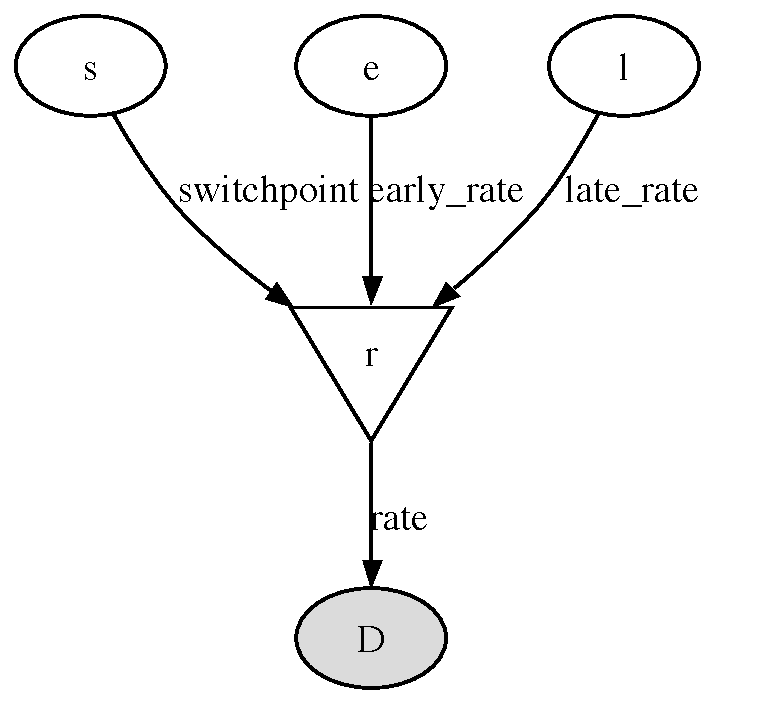
\epsfig{file=DisasterModel2.pdf, width=7cm}
    \caption{Graphical representation of the coal mining disaster model example.}
	\label{fig:disaster-dag}
\end{center}
\end{figure}


% Note that if a deterministic variable has more than one child, its parents each inherit all of its children when it is made implicit:
% \begin{center}
%     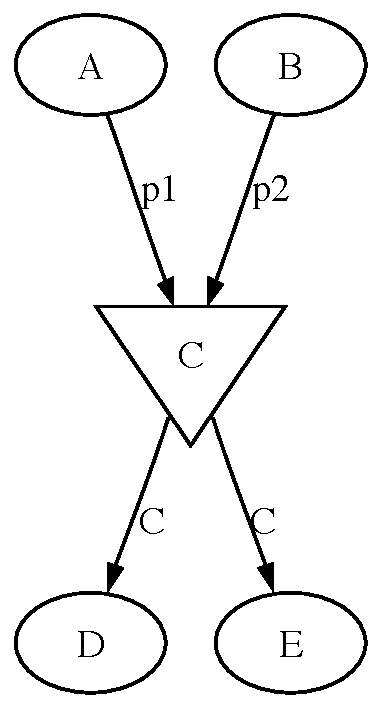
\epsfig{file=DeterministicPreInheritance.pdf, width=3.5cm} $\Rightarrow$ 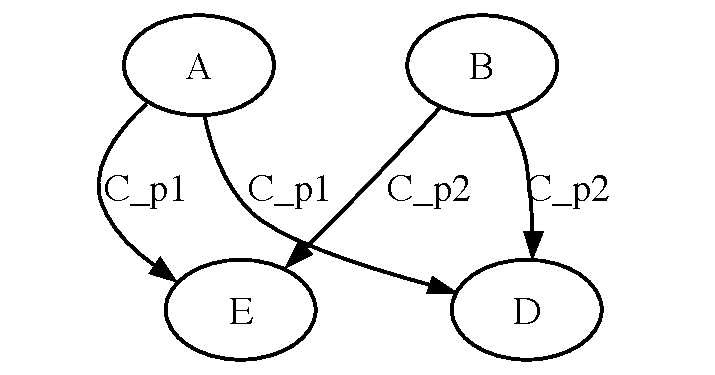
\epsfig{file=DeterministicPostInheritance.pdf, width=5cm}
% \end{center}
% These inherited children can be accessed via the \code{extended_children} attributes of the parents.

\begin{figure}[h!]
\begin{center}
    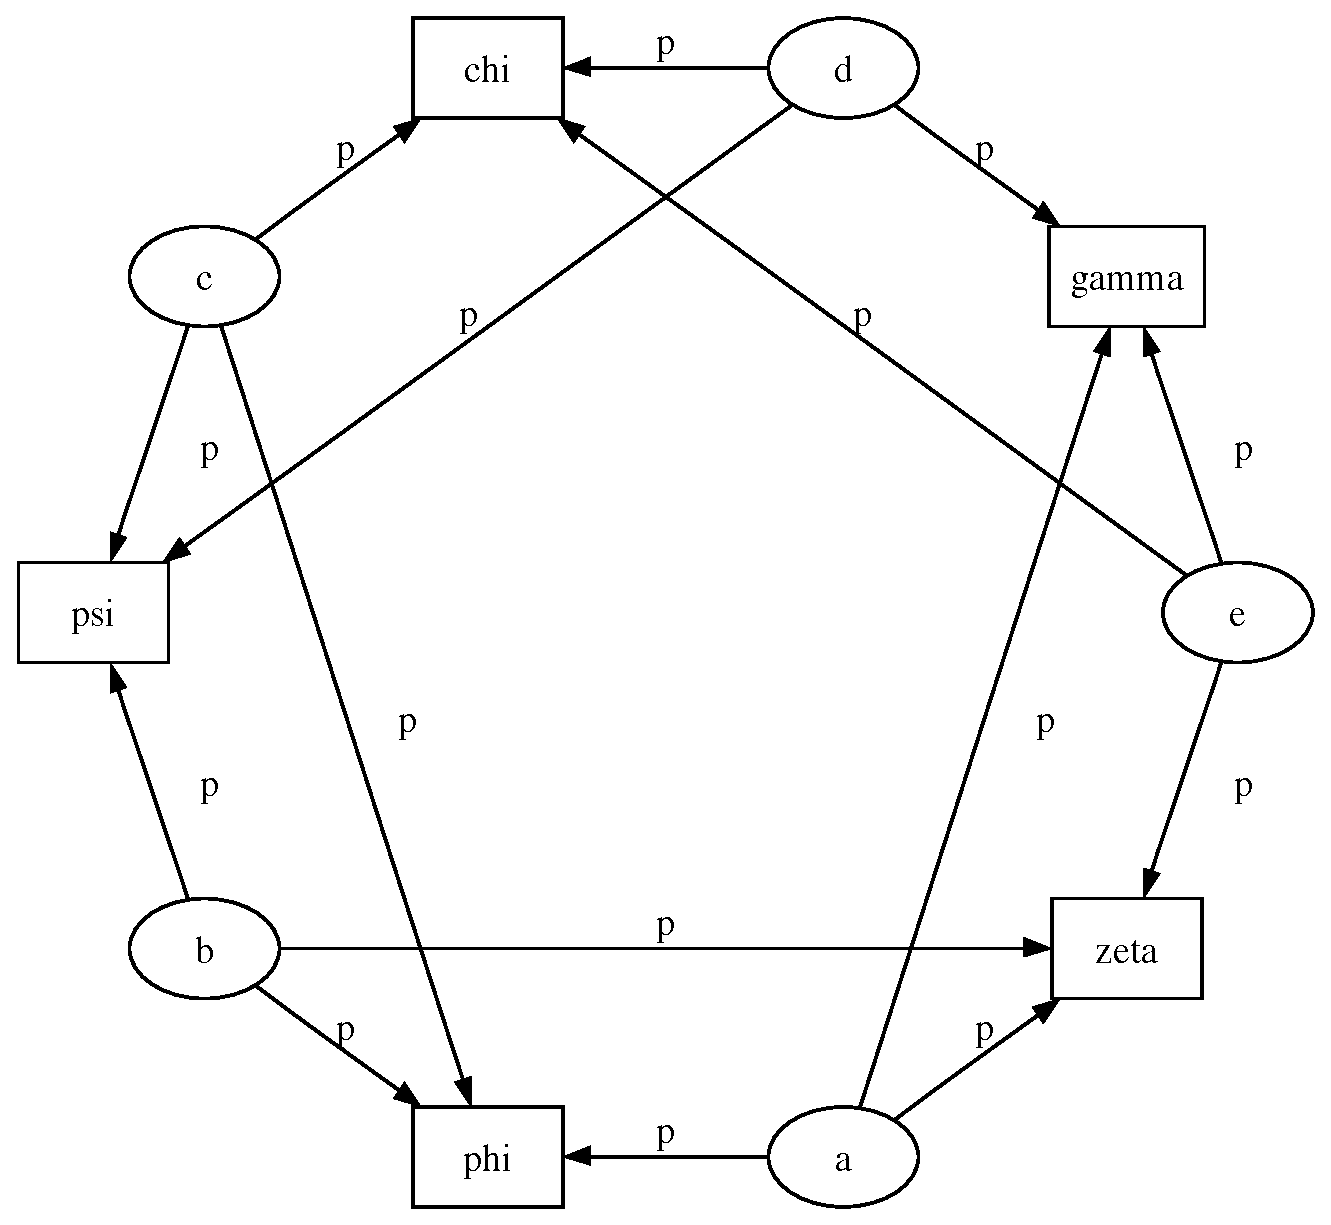
\epsfig{file=PotExample.pdf, width=12cm}
    \caption{Directed graphical model example. Factor potentials are represented by rectangles and stochastic variables by ellipses.}
    \label{fig:dgm}
\end{center}
\end{figure}

The symbol for factor potentials is a rectangle (Figure~\ref{fig:dgm}). Factor potentials are usually associated with \emph{undirected} grahical models. In undirected representations, each parent of a potential is connected to every other parent by an undirected edge. The undirected representation of the model is much more compact (Figure~\ref{fig:dgm-collapsed}). Directed or mixed graphical models can be represented in an undirected form by `moralizing', which is done by the function \code{pymc.graph.moral_graph}.

\begin{figure}[h!]
\begin{center}
    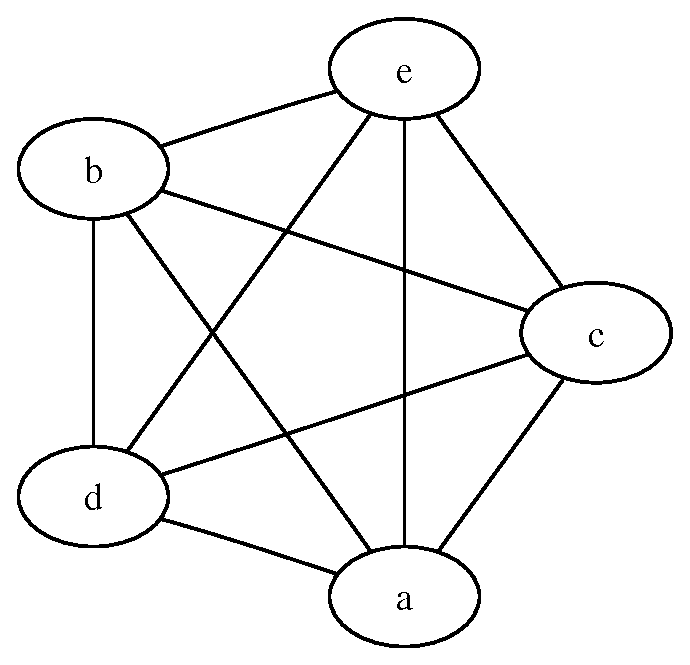
\epsfig{file=PotExampleCollapsed.pdf, width=10cm}
    \caption{The undirected version of the graphical model of figure~\ref{fig:dgm}.}
	\label{fig:dgm-collapsed}
\end{center}
\end{figure}


\subsection[Class LazyFunction and caching]{Class \code{LazyFunction}
and caching}
\label{sec:caching}
This Section~gives an overview of how \pkg{PyMC} computes log-probabilities. This is advanced information that is not required in order to use \pkg{PyMC}.

The \code{logp} attributes of stochastic variables and potentials and the \code{value} attributes of deterministic variables are wrappers for instances of class \code{LazyFunction}. Lazy functions are wrappers for ordinary \proglang{Python} functions. A lazy function \code{L} could be created from a function \code{fun} as follows:
\begin{CodeInput}
L = pm.LazyFunction(fun, arguments)
\end{CodeInput}
The argument \code{arguments} is a dictionary container; \code{fun} must accept keyword arguments only. When \code{L}'s \code{get()} method is called, the return value is the same as the call
\begin{CodeInput}
fun(**arguments.value)
\end{CodeInput}
Note that no arguments need to be passed to \code{L.get}; lazy functions memorize their arguments.

Before calling \code{fun}, \code{L} will check the values of its arguments' extended children against an internal cache. This comparison is done \emph{by reference}, not by value, and this is part of the reason why stochastic variables' values cannot be updated in-place. If the arguments' extended children's values match a frame of the cache, the corresponding output value is returned and \code{fun} is not called. If a call to \code{fun} is needed, the arguments' extended children's values and the return value replace the oldest frame in the cache. The depth of the cache can be set using the optional init argument \code{cache_depth}, which defaults to 2.

Caching is helpful in MCMC, because variables' log-probabilities and values tend to be queried multiple times for the same parental value configuration. The default cache depth of 2 turns out to be most useful in Metropolis-Hastings-type algorithms involving proposed values that may be rejected.

Lazy functions are implemented in C using \pkg{Pyrex} \citep{pyrex}, a language for writing \proglang{Python} extensions.



\section[Fitting Models]{Fitting models}
\label{chap:modelfitting}
% \pkg{PyMC} probability models are linked collections of nodes. These nodes are only informed by the values of their parents. \code{Deterministic} instances can compute their values given their parents' values, \code{Stochastic} instances can compute their log-probabilities or draw new values, and \code{Potential} instances can compute their log-probabilities. Fitting probability models requires larger-scale coordination and communication.

\pkg{PyMC} provides three objects that fit models:
\begin{itemize}
    \item \code{MCMC}, which coordinates Markov chain Monte Carlo algorithms. The actual work of updating stochastic variables conditional on the rest of the model is done by \code{StepMethod} objects, which are described in this section.
    \item \code{MAP}, which computes maximum \emph{a posteriori} estimates.
    \item \code{NormApprox}, which computes the `normal approximation' \citep{gelman}: the joint distribution of all stochastic variables in a model is approximated as normal using local information at the maximum \emph{a posteriori} estimate.
\end{itemize}

All three objects are subclasses of \code{Model}, which is \pkg{PyMC}'s base class for fitting methods. \code{MCMC} and \code{NormApprox}, both of which can produce samples from the posterior, are subclasses of \code{Sampler}, which is \pkg{PyMC}'s base class for Monte Carlo fitting methods. \code{Sampler} provides a generic sampling loop method and database support for storing large sets of joint samples. These base classes are documented at the end of this section. %Sampling loops can optionally be run interactively, meaning the user can pause sampling at any time, return to the \proglang{Python} prompt, check progress, and make adjustments.

\subsection{Creating models} \label{sec:ModelInstantiation}
The first argument to any fitting method's \code{init} method, including that of \code{MCMC}, is called \code{input}. The \code{input} argument can be just about anything; once you have defined the nodes that make up your model, you shouldn't even have to think about how to wrap them in a \code{Model} instance. Some examples of model instantiation using nodes \code{a}, \code{b} and \code{c} follow:
\begin{itemize}
    \item \code{M = Model(set([a,b,c]))}
    \item \code{M = Model(\{`a': a, `d': [b,c]\})} In this case, $M$ will expose $a$ and $d$ as attributes: \code{M.a} will be $a$, and \code{M.d} will be \code{[b,c]}.
    \item \code{M = Model([[a,b],c])}
    \item If file \code{MyModule} contains the definitions of \code{a}, \code{b} and \code{c}:
   \begin{CodeInput}
import MyModule
M = Model(MyModule)
\end{CodeInput}
    In this case, $M$ will expose $a$, $b$ and $c$ as attributes.
    \item Using a `model factory' function:
    \begin{CodeInput}
def make_model(x):
	a = pm.Exponential('a',beta=x,value=0.5)

@pm.deterministic
def b(a=a):
    return 100-a

@pm.stochastic
def c(value=0.5, a=a, b=b):
    return (value-a)**2/b

return locals()

M = pm.Model(make_model(3))
\end{CodeInput}
    In this case, $M$ will also expose $a$, $b$ and $c$ as attributes.
\end{itemize}

\subsection[The Model class]{The \code{Model} class} \label{sec:Model}
\code{Model} serves as a container for probability models and as a base class for the classes responsible for model fitting, such as \code{MCMC}.

\code{Model}'s init method takes the following arguments:
\begin{description}
    \item[\code{input}:] Some collection of \pkg{PyMC} nodes defining a probability model. These may be stored in a list, set, tuple, dictionary, array, module, or any object with a \code{__dict__} attribute.
    \item[\code{verbose} (optional):] An integer controlling the verbosity of the model's output.
\end{description}

Models' useful methods are:
\begin{description}
    \item[\code{draw_from_prior()}:] Sets all stochastic variables' values to new random values, which would be a sample from the joint distribution if all data and \code{Potential} instances' log-probability functions returned zero. If any stochastic variables lack a \code{random()} method, \pkg{PyMC} will raise an exception.
    \item[\code{seed()}:] Same as \code{draw_from_prior}, but only \code{stochastics} whose \code{rseed} attribute is not \code{None} are changed.
\end{description}

The helper function \code{graph} produces graphical representations of models \cite[see]{Jordan:2004p5439}.

Models have the following important attributes:
\begin{itemize}
    \item \code{variables}
    \item \code{stochastics}
    \item \code{potentials}
    \item \code{deterministics}
    \item \code{observed_stochastics}
    \item \code{step_methods}
    \item \code{value}: A copy of the model, with each attribute that is a \pkg{PyMC} variable or container replaced by its value.
    \item \code{generations}: A topological sorting of the stochastics in the model.
\end{itemize}

In addition, models expose each node they contain as an attribute. For instance, if model \code{M} were produced from model (\ref{disastermodel}) \code{M.s} would return the switchpoint variable.


\subsection{Maximum a posteriori estimates} \label{sec:MAP}

The \code{MAP} class sets all stochastic variables to their maximum \emph{a posteriori} values using functions in \pkg{SciPy}'s \code{optimize} package. \pkg{SciPy} must be installed to use it. \code{MAP} can only handle variables whose dtype is \code{float}, so it will not work on model \ref{disastermodel}. To fit the model in \code{examples/gelman_bioassay.py} using \code{MAP}, do the following
\begin{CodeInput}
>>> from pymc.examples import gelman_bioassay
>>> M = pm.MAP(gelman_bioassay)
>>> M.fit()
\end{CodeInput}
This call will cause $M$ to fit the model using Nelder-Mead optimization, which does not require derivatives. The variables in \code{gelman_bioassay} have now been set to their maximum \emph{a posteriori} values:
\begin{CodeInput}
>>> M.alpha.value
array(0.8465892309923545)
>>> M.beta.value
array(7.7488499785334168)
\end{CodeInput}
In addition, the AIC and BIC of the model are now available:
\begin{CodeInput}
>>> M.AIC
7.9648372671389458
>>> M.BIC
6.7374259893787265
\end{CodeInput}

\bigskip
\code{MAP} has two useful methods:
\begin{description}
    \item[\code{fit(method ='fmin', iterlim=1000, tol=.0001)}:] The optimization method may be \code{fmin}, \code{fmin_l_bfgs_b}, \code{fmin_ncg}, \code{fmin_cg}, or \code{fmin_powell}. See the documentation of \pkg{SciPy}'s \code{optimize} package for the details of these methods. The \code{tol} and \code{iterlim} parameters are passed to the optimization function under the appropriate names.
    \item[\code{revert_to_max()}:] If the values of the constituent stochastic variables change after fitting, this function will reset them to their maximum \emph{a posteriori} values.
\end{description}
If you're going to use an optimization method that requires derivatives, \code{MAP}'s \code{init} method can take additional parameters \code{eps} and \code{diff_order}. \code{diff_order}, which must be an integer, specifies the order of the numerical approximation (see the \pkg{SciPy} function \code{derivative}). The step size for numerical derivatives is controlled by \code{eps}, which may be either a single value or a dictionary of values whose keys are variables (actual objects, not names).

The useful attributes of \code{MAP} are:
\begin{description}
    \item[\code{logp}:] The joint log-probability of the model.
    \item[\code{logp_at_max}:] The maximum joint log-probability of the model.
    % \item[\code{len}:] The total number of elements in all the stochastic variables in the model with \code{observed=False}.
    % \item[\code{data_len}:] The total number number of elements in all the stochastic variables in the model with \code{observed=True}.
    \item[\code{AIC}:] Akaike's information criterion for this model \citep{Akaike:1973aj,Burnham:2002ic}.
    \item[\code{BIC}:] The Bayesian information criterion for this model \citep{Schwarz:1978ud}.
\end{description}

One use of the \code{MAP} class is finding reasonable initial states for MCMC chains. Note that multiple \code{Model} subclasses can handle the same collection of nodes.

\subsection{Normal approximations} \label{sec:norm-approx}

The \code{NormApprox} class extends the \code{MAP} class by approximating the posterior covariance of the model using the Fisher information matrix, or the Hessian of the joint log probability at the maximum. To fit the model in \code{examples/gelman_bioassay.py} using \code{NormApprox}, do:
\begin{CodeInput}
>>> N = pm.NormApprox(gelman_bioassay)
>>> N.fit()
\end{CodeInput}
The approximate joint posterior mean and covariance of the variables are available via the attributes \code{mu} and \code{C}:
\begin{CodeInput}
>>> N.mu[N.alpha]
array([ 0.84658923])
>>> N.mu[N.alpha, N.beta]
array([ 0.84658923,  7.74884998])
>>> N.C[N.alpha]
matrix([[ 1.03854093]])
>>> N.C[N.alpha, N.beta]
matrix([[  1.03854093,   3.54601911],
    [  3.54601911,  23.74406919]])
\end{CodeInput}
As with \code{MAP}, the variables have been set to their maximum \emph{a posteriori} values (which are also in the \code{mu} attribute) and the AIC and BIC of the model are available.

In addition, it's now possible to generate samples from the posterior as with \code{MCMC}:
\begin{CodeInput}
>>> N.sample(100)
>>> N.trace('alpha')[::10]
array([-0.85001278,  1.58982854,  1.0388088 ,  0.07626688,  1.15359581,
   -0.25211939,  1.39264616,  0.22551586,  2.69729987,  1.21722872])
>>> N.trace('beta')[::10]
array([  2.50203663,  14.73815047,  11.32166303,   0.43115426,
    10.1182532 ,   7.4063525 ,  11.58584317,   8.99331152,
    11.04720439,   9.5084239 ])
\end{CodeInput}
Any of the database backends can be used (Section~\ref{chap:database}).

\bigskip
In addition to the methods and attributes of \code{MAP}, \code{NormApprox} provides the following methods:
\begin{description}
    \item[\code{sample(iter)}:] Samples from the approximate posterior distribution are drawn and stored.
    \item[\code{isample(iter)}:] An `interactive' version of \code{sample()}: sampling can be paused, returning control to the user.
    \item[\code{draw}:] Sets all variables to random values drawn from the approximate posterior.
\end{description}
It provides the following additional attributes:
\begin{description}
    \item[\code{mu}:] A special dictionary-like object that can be keyed with multiple variables. \code{N.mu[p1, p2, p3]} would return the approximate posterior mean values of stochastic variables \code{p1}, \code{p2} and \code{p3}, ravelled and concatenated to form a vector.
    \item[\code{C}:] Another special dictionary-like object. \code{N.C[p1, p2, p3]} would return the approximate posterior covariance matrix of stochastic variables \code{p1}, \code{p2} and \code{p3}. As with \code{mu}, these variables' values are ravelled and concatenated before their covariance matrix is constructed.
\end{description}

\subsection[Markov chain Monte Carlo: the MCMC class]{Markov chain Monte
Carlo: the \code{MCMC} class} \label{sec:mcmc}

The \code{MCMC} class implements \pkg{PyMC}'s core business: producing Markov chains from a model's variables which can be considered sequences of joint samples from the posterior. See Section~\ref{chap:tutorial} for an example of basic usage.

\code{MCMC}'s primary job is to create and coordinate a collection of `step methods', each of which is responsible for updating one or more variables. The available step methods are described below. Instructions on how to create your own step method are available in Section~\ref{chap:extending}.

\code{MCMC} provides the following useful methods:
\begin{description}
    \item[\code{sample(iter, burn, thin, tune\_interval, tune\_throughout, save\_interval, verbose)}:] Runs the MCMC algorithm and produces the traces. The \code{iter} argument controls the total number of MCMC iterations. No tallying will be done during the first \code{burn} iterations; these samples will be forgotten. After this burn-in period, tallying will be done each \code{thin} iterations. Tuning will be done each \code{tune\_interval} iterations. If \code{tune\_throughout=False}, no more tuning will be done after the burnin period. The model state will be saved every \code{save\_interval} iterations, if given.
    \item[\code{isample(iter, burn, thin, tune\_interval, tune\_throughout, save\_interval, verbose)}:] An interactive version of \code{sample}. The sampling loop may be paused at any time, returning control to the user.
    \item[\code{use_step_method(method, *args, **kwargs)}:] Creates an instance of step method class \code{method} to handle some stochastic variables. The extra arguments are passed to the \code{init} method of \code{method}. Assigning a step method to a variable manually will prevent the \code{MCMC} instance from automatically assigning one. However, you may handle a variable with multiple step methods.
    % \item[\code{assign_step_methods()}:] Assigns step methods to all stochastic variables that do not currently have any. This method is called whenever \code{sample} or \code{isample} is called, but it can be useful to call it directly to see what the default step methods will be.

    % A variable is assigned a step method as follows: each eligible \code{StepMethod} subclass in existence is allowed to inspect the variable in question and determine its competence to handle the variable, on a scale of 0 to 3. An instance of the highest bidder is created to handle the variable.
    \item[\code{goodness()}:] Calculates goodness-of-fit (GOF) statistics according to \citet{Brooks:2000il}.
    \item[\code{save\_state()}:] Saves the current state of the sampler, including all stochastics, to the database. This allows the sampler to be reconstituted at a later time to resume sampling. This is not supported yet for the RDBMS backends, \code{sqlite} and \code{mysql}.
    \item[\code{restore\_state()}:] Restores the sampler to the state stored in the database.
   \item[\code{stats()}:] Generates summary statistics for all nodes in the model.
    \item[\code{remember(trace\_index)}:] Set all variables' values from frame \code{trace\_index} in the database.
\end{description}

MCMC samplers' step methods can be accessed via the \code{\textbf{step_method_dict}} attribute. \\\code{M.step_method_dict[x]} returns a list of the step methods \code{M} will use to handle the stochastic variable \code{x}.

After sampling, the information tallied by \code{M}  can be queried via \code{M.db.trace_names}. In addition to the values of variables, tuning information for adaptive step methods is generally tallied. These `traces' can be plotted to verify that tuning has in fact terminated.

You can produce `traces' for arbitrary functions with zero arguments as well. If you issue the command \code{M._funs_to_tally['trace_name'] = f} before sampling begins, then each time the model variables' values are tallied \code{f} will be called with no arguments, and the return value will be tallied. After sampling ends you can retrieve the trace as \code{M.trace['trace_name']}

\subsection[The Sampler class]{The \code{Sampler} class} \label{sec:Sampler}
\code{MCMC} is a subclass of a more general class called \code{Sampler}. Samplers fit models with Monte Carlo fitting methods, which characterize the posterior distribution by approximate samples from it. They are initialized as follows: \code{Sampler(input=None, db='ram', name='Sampler', reinit_model=True, calc_deviance=False)}. The \code{input} argument is a module, list, tuple, dictionary, set, or object that contains all elements of the model, the \code{db} argument indicates which database backend should be used to store the samples (see Section~\ref{chap:database}), \code{reinit\_model} is a boolean flag that indicates whether the model should be re-initialised before running, and \code{calc\_deviance} is a boolean flag indicating whether deviance should be calculated for the model at each iteration. Samplers have the following important methods:
\begin{description}
    \item[\code{sample(iter, length=None, verbose=0)}:] Samples from the joint distribution. The \code{iter} argument controls how many times the sampling loop will be run, and the \code{length} argument controls the initial size of the database that will be used to store the samples.
    \item[\code{isample(iter, length=None, verbose=0)}:] The same as \code{sample}, but the sampling is done interactively: you can pause sampling at any point and be returned to the \proglang{Python} prompt to inspect progress and adjust fitting parameters. While sampling is paused, the following methods are useful:
    \begin{description}
        \item[\code{icontinue()}:] Continue interactive sampling.
        \item[\code{halt()}:] Truncate the database and clean up.
    \end{description}
    \item[\code{tally()}:] Write all variables' current values to the database. The actual write operation depends on the specified database backend.
    %\item[\code{draw()}:] Not currently used. In future Monte Carlo fitting methods that aren't MCMC, such as importance samplers, the \code{draw()} method will be responsible for drawing approximate samples from the joint distribution (by setting the values of all the stochastic variables in the model).
    \item[\code{save\_state()}:] Saves the current state of the sampler, including all stochastics, to the database. This allows the sampler to be reconstituted at a later time to resume sampling. This is not supported yet for the RDBMS backends, sqlite and mysql.
    \item[\code{restore\_state()}:] Restores the sampler to the state stored in the database.
   \item[\code{stats()}:] Generates summary statistics for all nodes in the model.
    \item[\code{remember(trace\_index)}:] Set all variables' values from frame \code{trace\_index} in the database. Note that the \code{trace_index} is different from the current iteration, since not all samples are necessarily saved due to burning and thinning.
\end{description}

In addition, the sampler attribute \code{deviance} is a deterministic variable valued as the model's deviance at its current state.


\subsection{Step methods} \label{sec:stepmethod}


Step method objects handle individual stochastic variables, or sometimes groups of them. They are responsible for making the variables they handle take single MCMC steps conditional on the rest of the model. Each subclass of \code{StepMethod} implements a method called \code{step()}, which is called by \code{MCMC}. Step methods with adaptive tuning parameters can optionally implement a method called \code{tune()}, which causes them to assess performance (based on the acceptance rates of proposed values for the variable) so far and adjust.

The major subclasses of \code{StepMethod} are \code{Metropolis},
\code{AdaptiveMetropolis} and \code{Gibbs}. \pkg{PyMC} provides several flavors of the
basic Metropolis steps, but the Gibbs steps are not ready for use as of the
current release. However, because it is feasible to write Gibbs step methods
for particular applications, the \code{Gibbs} base class will be documented
here.

\subsection{Metropolis step methods} \label{metropolis}

\code{Metropolis} and subclasses implement Metropolis-Hastings steps. To tell an \code{MCMC} object $M$ to handle a variable $x$ with a Metropolis step method, you might do the following:
\begin{CodeInput}
M.use_step_method(pm.Metropolis, x, proposal_sd=1., \ 
    proposal_distribution='Normal')
\end{CodeInput}

\code{Metropolis} itself handles float-valued variables, and subclasses \code{DiscreteMetropolis} and \code{BinaryMetropolis} handle integer- and boolean-valued variables, respectively. Subclasses of \code{Metropolis} must implement the following methods:
\begin{description}
    \item[\code{propose()}:] Sets the values of the variables handled by the Metropolis step method to proposed values.
    \item[\code{reject()}:] If the Metropolis-Hastings acceptance test fails, this method is called to reset the values of the variables to their values before \code{propose()} was called.
\end{description}
Note that there is no \code{accept()} method; if a proposal is accepted, the variables' values are simply left alone. Subclasses that use proposal distributions other than symmetric random-walk may specify the `Hastings factor' by changing the \code{hastings\_factor} method. See Section~\ref{chap:extending} for an example.

\code{Metropolis}' \code{init} method takes the following arguments:
\begin{description}
   \item[\code{stochastic}:] The variable to handle.
   \item[\code{proposal_sd}:] A float or array of floats. This sets the
    default proposal standard deviation if the proposal distribution is normal.
   \item[\code{scale}:] A float, defaulting to 1. If the \code{scale} argument is provided but not \code{proposal_sd}, \code{proposal\_sd} is computed as follows:
   \begin{CodeInput}
if all(self.stochastic.value != 0.):
   self.proposal_sd = ones(shape(self.stochastic.value)) * \
                       abs(self.stochastic.value) * scale
else:
   self.proposal_sd = ones(shape(self.stochastic.value)) * scale
\end{CodeInput}
   \item[\code{proposal_distribution}:] A string indicating which distribution should be used for proposals. Current options are \code{`Normal'} and \code{`Prior'}. If \code{proposal_distribution=None}, the proposal distribution is chosen automatically. It is set to \code{`Prior'} if the variable has no children and has a random method, and to \code{`Normal'} otherwise.
   \item[\code{verbose}:] An integer. By convention, $0$ indicates minimal output and $2$ indicates maximum verbosity.
\end{description}

Although the \code{proposal\_sd} attribute is fixed at creation, Metropolis step methods adjust this initial value using an attribute called \code{adaptive_scale_factor}. When \code{tune()} is called, the acceptance ratio of the step method is examined and this scale factor is updated accordingly. If the proposal distribution is normal, proposals will have standard deviation \code{self.proposal\_sd * self.adaptive_scale_factor}.

By default, tuning will continue throughout the sampling loop, even after the burnin period is over. This can be changed via the \code{tune\_throughout} argument to \code{MCMC.sample}. If an adaptive step method's \code{tally} flag is set (the default for \code{Metropolis}), a trace of its tuning parameters will be kept. If you allow tuning to continue throughout the sampling loop, it is important to verify that the `Diminishing Tuning' condition of \citet{tuning} is satisfied: the amount of tuning should decrease to zero, or tuning should become very infrequent.

If a Metropolis step method handles an array-valued variable, it proposes all elements independently but simultaneously. That is, it decides whether to accept or reject all elements together but it does not attempt to take the posterior correlation between elements into account. The \code{AdaptiveMetropolis} class (see below), on the other hand, does make correlated proposals.

\subsection[The AdaptiveMetropolis class]{The \code{AdaptiveMetropolis} class}
\label{subsec:AM}
The \code{AdaptativeMetropolis} (AM) step method works like a regular Metropolis
step method, with the exception that its variables are block-updated using a
multivariate jump distribution whose covariance is tuned during sampling.
Although the chain is non-Markovian, it has correct ergodic properties (see
\citet{Haario:2001lr}).

To tell an \code{MCMC} object $M$ to handle variables $x$, $y$ and $z$ with an
\code{AdaptiveMetropolis} instance, you might do the following:
\begin{CodeInput}
M.use_step_method(pm.AdaptiveMetropolis, [x,y,z], \
                  scales={x:1, y:2, z:.5}, delay=10000)
\end{CodeInput}

\code{AdaptativeMetropolis}' init method takes the following arguments:
% cov=None, delay=1000, scales=None, interval=200, greedy=True,verbose=0
\begin{description}
   \item[\code{stochastics}:] The stochastic variables to handle. These will be
updated jointly.
   \item[\code{cov} (optional):] An initial covariance matrix. Defaults to the
identity matrix, adjusted according to the \code{scales} argument.
   \item[\code{delay} (optional):] The number of iterations to delay before
computing the empirical covariance matrix.
   \item[\code{scales} (optional):] The initial covariance matrix will be
diagonal, and its diagonal elements will be set to \code{scales} times the
stochastics' values, squared.
   \item[\code{interval} (optional):] The number of iterations between updates
of the covariance matrix. Defaults to 1000.
   \item[\code{greedy} (optional):] If \code{True}, only accepted jumps will be
counted toward the delay before the covariance is first computed. Defaults to
\code{True}.
   \item[\code{verbose} (optional):] An integer from 0 to 3 controlling the verbosity of
the step method's printed output.
    \item[\code{shrink_if_necessary} (optional):] Whether the proposal covariance should be
shrunk if the acceptance rate becomes extremely small.
\end{description}

In this algorithm, jumps are proposed from a multivariate normal
distribution with covariance matrix $C$. The algorithm first iterates
until \code{delay} samples have been drawn (if \code{greedy} is true, until
\code{delay} jumps have been accepted). At this point, $C$ is given
the value of the empirical covariance of the trace so far and sampling
resumes. The covariance is then updated each \code{interval}
iterations throughout the entire sampling run\footnote{The covariance is
estimated recursively from the previous value and the last \code{interval}
samples, instead of computing it each time from the entire trace.}. It is
this constant adaptation of the proposal distribution that makes the chain
non-Markovian.

\subsection[The DiscreteMetropolis class]{The
\code{DiscreteMetropolis} class}
This class is just like \code{Metropolis}, but specialized to handle
\code{Stochastic} instances with dtype \code{int}. The jump proposal
distribution can either be \code{`Normal'}, \code{`Prior'} or \code{`Poisson'}.
In the normal case, the proposed value is drawn from a normal distribution
centered at the current value and then rounded to the
nearest integer. In the Poisson case, the proposed value is obtained by adding
or substracting (with equal probability) a random value drawn from a Poisson
distribution.

\subsection[The BinaryMetropolis class]{The
\code{BinaryMetropolis} class}
This class is specialized to handle \code{Stochastic} instances with dtype
\code{bool}.

For array-valued variables, \code{BinaryMetropolis} can be set to propose from
the prior by passing in \code{dist="Prior"}. Otherwise, the argument
\code{p_jump} of the init method specifies how probable a change is. Like
\code{Metropolis}' attribute \code{proposal_sd}, \code{p_jump} is tuned
throughout the sampling loop via \code{adaptive_scale_factor}.

For scalar-valued variables, \code{BinaryMetropolis} behaves like a Gibbs
sampler, since this requires no additional expense. The \code{p_jump} and
\code{adaptive_scale_factor} parameters are not used in this case.

\subsection{Granularity of step methods: one-at-a-time vs. block updating}
\label{subsec:granularity}
There is currently no way for a stochastic variable to compute individual terms of its log-probability; it is computed all together. This means that updating the elements of a array-valued variable individually would be inefficient, so all existing step methods update array-valued variables together, in a block update.

To update an array-valued variable's elements individually, simply break it up into an array of scalar-valued variables. Instead of this:
\begin{CodeInput}
A = pm.Normal('A', value=numpy.zeros(100), mu=0., tau=1.)
\end{CodeInput}
do this:
\begin{CodeInput}
A = [pm.Normal('A_%i'%i, value=0., mu=0., tau=1.) for i in range(100)]
\end{CodeInput}
An individual step method will be assigned to each element of \code{A} in the latter case, and the elements will be updated individually. Note that \code{A} can be broken up into larger blocks if desired.

\subsection{Automatic assignment of step methods}
Every step method subclass (including user-defined ones) that does not require any \code{init} arguments other than the stochastic variable to be handled adds itself to a list called \\\code{StepMethodRegistry} in the \pkg{PyMC} namespace. If a stochastic variable in an \code{MCMC} object has not been explicitly assigned a step method, each class in \code{StepMethodRegistry} is allowed to examine the variable.

To do so, each step method implements a class method called \code{competence}, whose only argument is a single stochastic variable. These methods return values from 0 to 3; 0 meaning the step method cannot safely handle the variable and 3 meaning it will most likely be the best available step method for variables like this. The \code{MCMC} object assigns the step method that returns the highest competence value to each of its stochastic variables.

\section[Sampling Results]{Saving and managing sampling results}
\label{chap:database}


\subsection{Accessing Sampled Data}
  \label{accessing-sampled-data}%


The recommended way to access data from an MCMC run, irrespective of the
database backend, is to use the \code{trace} method:
%
\begin{CodeInput}
>>> from pymc.examples import DisasterModel
>>> M = pm.MCMC(DisasterModel)
>>> M.sample(10)
>>> M.trace('e')[:]
array([ 2.28320992,  2.28320992,  2.28320992,  2.28320992,  2.28320992,
        2.36982455,  2.36982455,  3.1669422 ,  3.1669422 ,  3.14499489])    
\end{CodeInput}

\code{M.trace('e')} returns a copy of the \code{Trace} instance belonging to
the tallyable object $e$:
\begin{CodeInput}
>>> M.trace('e')
<pymc.database.ram.Trace object at 0x7fa4877a8b50>
\end{CodeInput}

Samples from the trace are obtained using the slice notation \code{{[}{]}},
similarly to \pkg{NumPy} arrays. By default, \code{trace} returns the samples from
the last chain. To return samples from all the chains, set
\code{chain=None}:
%

\begin{CodeInput}
>>> M.sample(5)
>>> M.trace('e', chain=None)[:]
array([ 2.28320992,  2.28320992,  2.28320992,  2.28320992,  2.28320992,
        2.36982455,  2.36982455,  3.1669422 ,  3.1669422 ,  3.14499489,
        3.14499489,  3.14499489,  3.14499489,  2.94672454,  3.10767686])    
\end{CodeInput}




%___________________________________________________________________________

\subsection{Saving Data to Disk}
  \label{saving-data-to-disk}%


By default, the database backend selected by the \code{MCMC} sampler is the \code{ram}
backend, which simply holds the data in RAM. Now, we create a
sampler that, instead, writes data to a pickle file:
%
\begin{CodeInput}
>>> M = pm.MCMC(DisasterModel, db='pickle', dbname='Disaster.pickle')
>>> M.db
<pymc.database.pickle.Database object at 0x7fa486623d90>

>>> M.sample(10)
>>> M.db.close()    
\end{CodeInput}

Note that in this particular case, no data is written to disk before the call
to \code{db.close}. The \code{close} method will flush data to disk and
prepare the database for a potential session exit. Closing a \proglang{Python} session
without calling \code{close} beforehand is likely to corrupt the database,
making the data irretrievable. To simply flush data to disk without
closing the database, use the \code{commit} method.

Some backends not only have the ability to store the traces, but also
the state of the step methods at the end of sampling. This is particularly
useful when long warm-up periods are needed to tune the jump parameters.
When the database is loaded in a new session, the step methods query
the database to fetch the state they were in at the end of the last trace.

Check that you \code{close} the database before closing the \proglang{Python} session.


%___________________________________________________________________________

\subsection{Loading Back a Database}
  \label{loading-back-a-database}%


To load a file created in a previous session, use the \code{load} function
from the appropriate backend:
%
\begin{CodeInput}
>>> db = pymc.database.pickle.load('Disaster.pickle')
>>> len(db.trace('e')[:])
10    
\end{CodeInput}

The \code{db} object also has a \code{trace} method identical to that of \code{Sampler}.
You can hence inspect the results of a model, even if you don't have the model
around.

To add a new trace to this file, we need to create an MCMC instance. This time,
instead of setting \code{db='pickle'}, we will pass the existing \code{Database}
instance and sample as usual. A new trace will be appended to the first:

\begin{CodeInput}
>>> M = MCMC(DisasterModel, db=db)
>>> M.sample(5)
>>> len(M.trace('e', chain=None)[:])
15
>>> M.db.close()    
\end{CodeInput}




%___________________________________________________________________________

\subsection[ram]{The \code{ram} backend}
  \label{ram}%


Used by default, this backend simply holds a copy in memory, with no output
written to disk. This is useful for short runs or testing. For long runs
generating large amount of data, using this backend may fill the available
memory, forcing the OS to store data in the cache, slowing down all other
applications.


%___________________________________________________________________________

\subsection[no_trace]{The \code{no_trace} backend}
  \label{no-trace}%


This backend simply does not store the trace. This may be useful for testing
purposes.


%___________________________________________________________________________

\subsection[txt]{The \code{txt} backend}
  \label{txt}%


With the \code{txt} backend, the data is written to disk in ASCII files.
More precisely, the \code{dbname} argument is used to create a top directory
into which chain directories, called \code{Chain\_<\#>}, are created each
time \code{sample} is called:
%

\begin{CodeInput}
dbname/
  Chain_0/
    <object0 name>.txt
    <object1 name>.txt
    ...
  Chain_1/
    <object0 name>.txt
    <object1 name>.txt
    ...
  ...    
\end{CodeInput}

In each one of these chain directories, files named \code{<variable name>.txt}
are created, storing the values of the variable as rows of text:
%

\begin{CodeInput}
# Variable: e
# Sample shape: (5,)
# Date: 2008-11-18 17:19:13.554188
3.033672373807017486e+00
3.033672373807017486e+00
...    
\end{CodeInput}

While the \code{txt} backend makes it easy to load data using other
applications and programming languages, it is not optimized for speed nor
memory efficiency. If you plan on generating and handling large datasets,
read on for better options.


%___________________________________________________________________________

\subsection[pickle]{The \code{pickle} backend}
  \label{pickle}%


The \code{pickle} database relies on the \code{cPickle} module to save the
traces. Use of this backend is appropriate for small scale,
short-lived projects. For longer term or larger projects, the \code{pickle}
backend should be avoided since the files it creates might be unreadable
across different \proglang{Python} versions. The pickled file is a simple dump of a
dictionary containing the \pkg{NumPy} arrays storing the traces, as well as
the state of the \code{Sampler}'s step methods.


%___________________________________________________________________________

\subsection[sqlite]{The \code{sqlite} backend}
  \label{sqlite}%


The \code{sqlite} backend is based on the python module \code{sqlite3} 
(a \proglang{Python} 2.5 built-in) . It opens an SQL database named \code{dbname},
and creates one table~per tallyable objects. The rows of this table
store a key, the chain index and the values of the objects:
%
\begin{CodeInput}
key (INT), trace (INT),  v1 (FLOAT), v2 (FLOAT), v3 (FLOAT) ...    
\end{CodeInput}

The key is autoincremented each time a new row is added to the table,
that is, each time \code{tally} is called by the sampler. Note that the
\code{savestate} feature is not implemented, that is, the state of the step
methods is not stored internally in the database.


%___________________________________________________________________________

\subsection[mysql]{The \code{mysql} backend}
  \label{mysql}%


The \code{mysql} backend depends on the \pkg{MySQL} library and its python wrapper
\pkg{MySQLdb} \citep{mysqldb}. Like the \code{sqlite} backend, it creates an \proglang{SQL} database containing
one table per tallyable object. The main difference with
\code{sqlite} is that it can connect to a remote database, provided the url and
port of the host server is given, along with a valid user name and password.
These parameters are passed when the \code{Sampler} is instantiated:
%
\begin{itemize}

\item \code{dbname} The name of the database file.
                    
\item \code{dbuser} The database user name.
                    
\item \code{dbpass} The user password for this database.
                    
\item \code{dbhost} The location of the database host.
                    
\item \code{dbport} The port number to use to reach the database host.

\item \code{dbmode} File mode.  Use \code{a} to append values, and \code{w}
to overwrite an existing database.

\end{itemize}

The \code{savestate} feature is not implemented in the \code{mysql} backend.


%___________________________________________________________________________

\subsection[hdf5]{The \code{hdf5} backend}
  \label{hdf5}%


The \code{hdf5} backend uses \pkg{pyTables} to save data in binary HDF5 format.
The \code{hdf5} database is fast and can store huge traces, far larger than the
available RAM. Data can be compressed and decompressed on the fly to
reduce the disk footprint.
Another feature of this backend is that it can store arbitrary objects.
Whereas most of the other backends are limited to numerical values, \code{hdf5}
can tally any object that can be pickled, opening the door for powerful and
exotic applications (see \code{pymc.gp}).

The internal structure of an HDF5 file storing both numerical values and
arbitrary objects is as follows:
%
\begin{CodeInput}
/ (root)
  /chain0/ (Group) 'Chain #0'
    /chain0/PyMCSamples (Table(N,)) 'PyMC Samples'
    /chain0/group0 (Group) 'Group storing objects.'
      /chain0/group0/<object0 name> (VLArray(N,)) '<object0 name> samples.'
      /chain0/group0/<object1 name> (VLArray(N,)) '<object1 name> samples.'
      ...
  /chain1/ (Group) 'Chain \#1'
    ...    
\end{CodeInput}

All standard numerical values are stored in a \code{Table}, while \code{objects}
are stored in individual \code{VLArrays}.

The \code{hdf5} Database takes the following parameters:
%
\begin{itemize}

\item \code{dbname} Name of the \pkg{hdf5} file.

\item \code{dbmode} File mode: \code{a}: append, \code{w}: overwrite,
\code{r}: read-only.

\item \code{dbcomplevel} : Compression level, 0: no compression, 9: maximal compression.

\item \code{dbcomplib} Compression library (\pkg{zlib}, \pkg{bzip2}, \pkg{LZO})

\end{itemize}

According the the \pkg{pyTables} manual, \pkg{zlib} \cite{zlib} has a fast decompression,
relatively slow compression, and a good compression ratio;
\pkg{LZO} \cite{lzo}  has a fast compression, but a low compression ratio;
and \pkg{bzip2} \cite{bzip2}  has an excellent compression ratio but requires more CPU. Note that
some of these compression algorithms require additional software to work (see
the \pkg{pyTables} manual).


%___________________________________________________________________________

\subsection{Writing a New Backend}
  \label{writing-a-new-backend}%


It is relatively easy to write a new backend for \code{\pkg{PyMC}}. The first step is to
look at the \\\code{database.base} module, which defines barebone \code{Database}
and \code{Trace} classes. This module contains documentation on the methods that
should be defined to get a working backend.

Testing your new backend should be fairly straightforward, since the
\code{test\_database} module contains a generic test class that can easily
be subclassed to check that the basic features required of all backends
are implemented and working properly.




\section[Model Checking]{Model checking and diagnostics}
\label{chap:modelchecking}

\subsection{Convergence Diagnostics} % (fold)
%\label{sec:convergence_diagnostics}

Valid inferences from sequences of MCMC samples are based on the assumption that samples are derived from the true posterior distribution of interest. Theory guarantees this condition as the number of iterations approaches infinity. It is important, therefore, to determine the minimum number of samples required to ensure a reasonable approximation to the target posterior density. Unfortunately, no universal threshold exists across all problems, so convergence must be assessed independently each time MCMC estimation is performed. The procedures for verifying convergence are collectively known as convergence diagnostics.

One approach to analyzing convergence is analytical, whereby the variance of the sample at different sections of the chain are compared to that of the limiting distribution. These methods use distance metrics to analyze convergence, or place theoretical bounds on the sample variance, and though they are promising, they are generally difficult to use and are not prominent in the MCMC literature. More common is a statistical approach to assessing convergence. Statistical techniques, rather than considering the properties of the theoretical target distribution, only consider the statistical properties of the observed chain. Reliance on the sample alone restricts such convergence criteria to heuristics, and hence, convergence cannot be guaranteed. Although evidence for lack of convergence using statistical convergence diagnostics will correctly imply lack of convergence in the chain, the absence of such evidence will not \emph{guarantee} convergence in the chain. Nevertheless, negative results for one or more criteria will provide some measure of assurance to users that their sample will provide valid inferences.

For most simple models, convergence will occur quickly, sometimes within the first several hundred iterations, after which all remaining samples of the chain may be used to calculate posterior quantities. For many more complex models, convergence requires a significantly longer burn-in period; sometimes  orders of magnitude more samples are needed. Frequently, lack of convergence will be caused by poor \emph{mixing} (Figure~\ref{fig:mix}). Mixing refers to the degree to which the Markov chain explores the support of the posterior distribution. Poor mixing may stem from inappropriate proposals (if one is using the Metropolis-Hastings sampler) or from attempting to estimate models with highly correlated variables.

\begin{figure}[ht]
\begin{center}
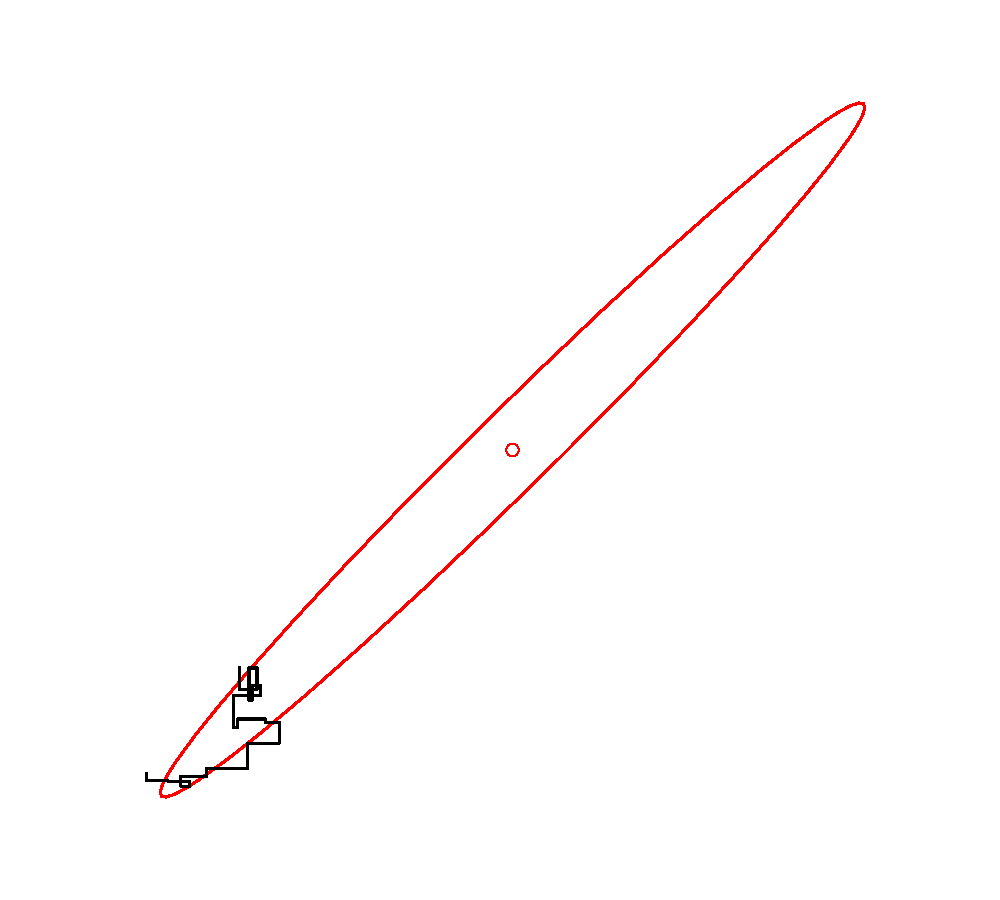
\includegraphics[height=3in]{poormixing.pdf}
\caption{An example of a poorly-mixing sample in two dimensions. Notice that the chain is trapped in a region of low probability relative to the mean (dot) and variance (oval) of the true posterior quantity.}
\label{fig:mix}
\end{center}
\end{figure}

\subsection{Informal Methods}

The most straightforward approach for assessing convergence is based on simply plotting and inspecting traces and histograms of the observed MCMC sample. If the trace of values for each of the stochastics exhibits asymptotic behaviour\footnote{Asymptotic behaviour implies that the variance and the mean value of the sample stays relatively constant over some arbitrary period.} over the last $m$ iterations, this may be satisfactory evidence for convergence. A similar approach involves plotting a histogram for every set of $k$ iterations (perhaps 50-100) beyond some burn-in threshold $n$; if the histograms are not visibly different among the sample intervals, this is some evidence for convergence. Note that such diagnostics should be carried out for each stochastic estimated by the MCMC algorithm, because convergent behaviour by one variable does not imply evidence for convergence for other variables in the model. An extension of this approach can be taken when multiple parallel chains are run, rather than just a single, long chain. In this case, the final values of $c$ chains run for $n$ iterations are plotted in a histogram; just as above, this is repeated every $k$ iterations thereafter, and the histograms of the endpoints are plotted again and compared to the previous histogram. This is repeated until consecutive histograms are indistinguishable.

\begin{figure}[h]
\begin{center}
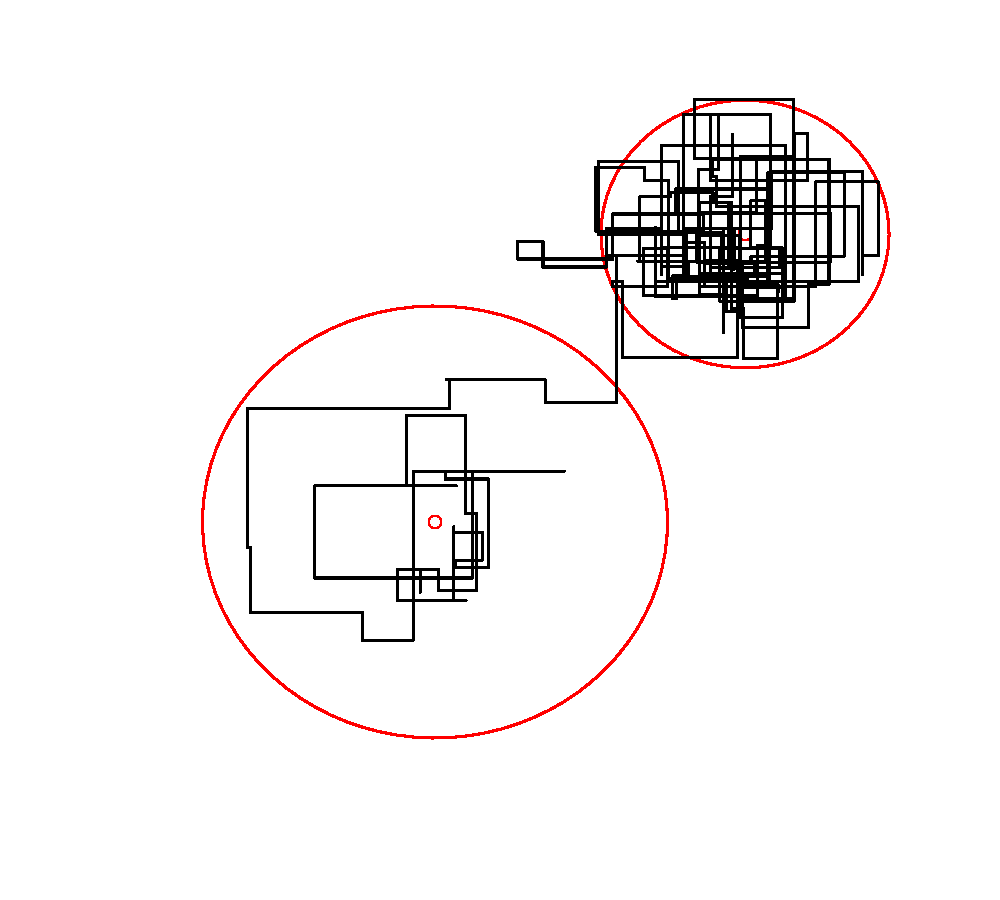
\includegraphics[height=3in]{metastable.pdf}
\caption{An example of metastability in a two-dimensional parameter space. The chain appears to be stable~in one region of the parameter space for an extended period, then unpredictably jumps to another region of the space.}
\label{fig:metas}
\end{center}
\end{figure}

Another \emph{ad hoc} method for detecting convergence is to examine the traces of several MCMC chains initialized with different starting values. Overlaying these traces on the same set of axes should (if convergence has occurred) show each chain tending toward the same equilibrium value, with approximately the same variance. Recall that the tendency for some Markov chains to converge to the true (unknown) value from diverse initial values is called \emph{ergodicity}. This property is guaranteed by the reversible chains constructed using MCMC, and should be observable using this technique. Again, however, this approach is only a heuristic method, and cannot always detect lack of convergence, even though chains may appear ergodic.

A principal reason that evidence from informal techniques cannot guarantee convergence is a phenomenon called metastability. Chains may appear to have converged to the true equilibrium value, displaying excellent qualities by any of the methods described above. However, after some period of stability around this value, the chain may suddenly move to another region of the parameter space (Figure~\ref{fig:metas}). This period of metastability can sometimes be very long, and therefore escape detection by these convergence diagnostics. Unfortunately, there is no statistical technique available for detecting metastability.

\subsection{Formal Methods}

Along with the \emph{ad hoc} techniques described above, a number of more formal methods exist which are prevalent in the literature. These are considered more formal because they are based on existing statistical methods, such as time series analysis.

\pkg{PyMC} currently includes functions for two formal convergence diagnostic procedures. The first, proposed by \citet{Geweke:1992gm}, is a time-series approach that compares the mean and variance of segments from the beginning and end of a single chain.
\begin{equation}
z = \frac{\bar{\theta}_a - \bar{\theta}_b}{\sqrt{Var(\theta_a) + Var(\theta_b)}}
\end{equation}
where $a$ is the early interval and $b$ the late interval. If the z-scores (theoretically distributed as standard normal variates) of these two segments are similar, it can provide evidence for convergence. \pkg{PyMC} calculates z-scores of the difference between various initial segments along the chain, and the last 50\% of the remaining chain. If the chain has converged, the majority of points should fall within 2 standard deviations of zero.

Diagnostic z-scores can be obtained by calling the \code{geweke} function. It accepts either (1) a single trace, (2) a Node or Stochastic object, or (3) an entire Model object:
\begin{CodeInput}
pm.geweke(pymc_object, first=0.1, last=0.5, intervals=20)
\end{CodeInput}
The arguments expected are the following
\begin{itemize}

\item \verb=pymc_object=: The object that is or contains the output trace(s).

\item \verb=first= (optional): First portion of chain to be used in Geweke diagnostic. Defaults to 0.1 (i.e. first 10\% of chain).

\item \verb=last= (optional): Last portion of chain to be used in Geweke diagnostic. Defaults to 0.5 (i.e. last 50\% of chain).

\item \verb=intervals= (optional): Number of sub-chains to analyze. Defaults to 20.
\end{itemize}

The resulting scores are best interpreted graphically, using the \code{geweke_plot} function. This displays the scores in series, in relation to the 2 standard deviation boundaries around zero. Hence, it is easy to see departures from the standard normal assumption.

\begin{figure}[h!]
\begin{center}
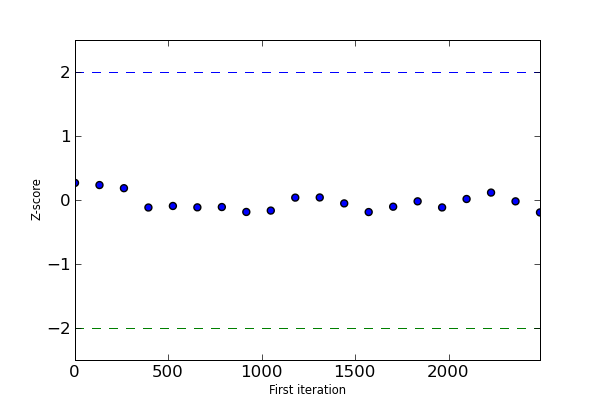
\includegraphics[height=18cm]{geweke.png}
\caption{Sample plots of Geweke z-scores for a variable using \textbf{geweke_plot}. The occurrence of the scores well within 2 standard deviations of zero gives does not indicate lack of convergence (top), while deviations exceeding 2 standard deviations suggests that additional samples are required to achieve convergence (bottom).}
\label{fig:geweke}
\end{center}
\end{figure}

\code{geweke_plot} takes either a single set of scores, or a dictionary of scores (output by \code{geweke} when an entire Sampler is passed) as its argument:
\begin{CodeInput}
geweke_plot(scores, name='geweke', format='png', suffix='-diagnostic', \
            path='./', fontmap = {1:10, 2:8, 3:6, 4:5, 5:4}, verbose=1)
\end{CodeInput}
\begin{itemize}

\item \verb=scores=: The object that contains the Geweke scores. Can be a list (one set) or a dictionary (multiple sets).

\item \verb=name= (optional): Name used for output files. For multiple scores, the dictionary keys are used as names.

\item \verb=format= (optional): Graphic output file format (defaults to \emph{png}).

\item \verb=suffix= (optional): Suffix to filename (defaults to \emph{-diagnostic})

\item \verb=path= (optional): The path for output graphics (defaults to working directory).

\item \verb=fontmap= (optional): Dictionary containing the font map for the labels of the graphic.

\item \verb=verbose= (optional): Verbosity level for output (defaults to 1).
\end{itemize}

To illustrate, consider a model \code{my_model} that is used to instantiate a MCMC sampler. The sampler is then run for a given number of iterations:
\begin{CodeInput}
>>> S = pm.MCMC(my_model)
>>> S.sample(10000, burn=5000)
\end{CodeInput}
It is easiest simply to pass the entire sampler \code{S} to the \code{geweke} function:
\begin{CodeInput}
>>> scores = pm.geweke(S, intervals=20)
>>> pm.Matplot.geweke_plot(scores)
\end{CodeInput}
Alternatively, individual stochastics within \code{S} can be analyzed for convergence:
\begin{CodeInput}
>>> trace = S.trace('alpha')[:]
>>> alpha_scores = pm.geweke(trace, intervals=20)
>>> pm.Matplot.geweke_plot(alpha_scores, 'alpha')
\end{CodeInput}
An example of convergence and non-convergence of a chain using \code{geweke_plot} is given in Figure~\ref{fig:geweke}. 


The second diagnostic provided by \pkg{PyMC} is the \citet{raftery} procedure. This approach estimates the number of iterations required to reach convergence, along with the number of burn-in samples to be discarded and the appropriate thinning interval. A separate estimate of both quantities can be obtained for each variable in a given model.

As the criterion for determining convergence, the Raftery and Lewis approach uses the accuracy of estimation of a user-specified quantile. For example, we may want to estimate the quantile $q=0.975$ to within $r=0.005$ with probability $s=0.95$. In other words,

\begin{equation}
  Pr(|\hat{q}-q| \le r) = s
\end{equation}

From any sample of $\theta$, one can construct a binary chain:

\begin{equation}
  Z^{(j)} = I(\theta^{(j)} \le u_q)
\end{equation}

where $u_q$ is the quantile value and $I$ is the indicator function. While $\{\theta^{(j)}\}$ is a Markov chain, $\{Z^{(j)}\}$ is not necessarily so. In any case, the serial dependency among $Z^{(j)}$ decreases as the thinning interval $k$ increases. A value of $k$ is chosen to be the smallest value such that the first order Markov chain is preferable to the second order Markov chain.

This thinned sample is used to determine number of burn-in samples. This is done by comparing the remaining samples from burn-in intervals of increasing length to the limiting distribution of the chain. An appropriate value is one for which the truncated sample's distribution is within $\epsilon$ (arbitrarily small) of the limiting distribution. See \citet{raftery} or \citet{Gamerman:1997tb} for computational details. Estimates for sample size tend to be conservative.

This diagnostic is best used on a short pilot run of a particular model, and the results used to parameterize a subsequent sample that is to be used for inference. Its calling convention is as follows:
\begin{CodeInput}
raftery_lewis(pymc_object, q, r, s=.95, epsilon=.001, verbose=1)
\end{CodeInput}
The arguments are:
\begin{itemize}

  \item \verb=pymc_object=: The object that contains the Geweke scores. Can be a list (one set) or a dictionary (multiple sets).

    \item \verb=q=: Desired quantile to be estimated.

    \item \verb=r=: Desired accuracy for quantile.

    \item \verb=s= (optional): Probability of attaining the requested accuracy (defaults to 0.95).

    \item \verb=epsilon= (optional) : Half width of the tolerance interval required for the q-quantile (defaults to 0.001).

    \item \verb=verbose= (optional) : Verbosity level for output (defaults to 1).
\end{itemize}

The code for \code{raftery_lewis} is based on the \proglang{Fortran}  program \pkg{gibbsit} \citep{gibbsit}.

For example, consider again a sampler \code{S} run for some model \code{my_model}:
\begin{CodeInput}
>>> S = pm.MCMC(my_model)
>>> S.sample(10000, burn=5000)
\end{CodeInput}
One can pass either the entire sampler \code{S} or any stochastic within \code{S} to the \code{raftery_lewis} function, along with suitable~arguments. Here, we have chosen $q=0.025$ (the lower limit of the equal-tailed 95\% interval) and error $r=0.01$:
\begin{CodeInput}
>>> pm.raftery_lewis(S, q=0.025, r=0.01)
\end{CodeInput}
This yields diagnostics as follows for each stochastic of \code{S}, as well as a dictionary containing the diagnostic quantities:

\begin{CodeInput}
========================
Raftery-Lewis Diagnostic
========================

937 iterations required (assuming independence) to achieve 0.01 accuracy
with 95 percent probability.

Thinning factor of 1 required to produce a first-order Markov chain.

39 iterations to be discarded at the beginning of the simulation (burn-in).

11380 subsequent iterations required.

Thinning factor of 11 required to produce an independence chain.
\end{CodeInput}

Additional convergence diagnostics are available in the
\proglang{r} language \citep{r}, via the
\pkg{CODA} module \citep{coda}. \pkg{PyMC} includes a method
\code{coda} for exporting model traces in a format that may be
directly read by CODA:
\begin{CodeInput}
pm.utils.coda(pymc_object)
\end{CodeInput}
The lone argument is the \pkg{PyMC} sampler for which output is desired.

Calling \verb=coda= yields two files, one containing raw trace values (suffix
\verb=.out=) and another containing indices to the trace values (suffix
\verb=.ind=).


\subsection{Autocorrelation Plots} % (fold)
%\label{sec:autocorrelation_plots}

Samples from MCMC algorithms are ususally autocorrelated, due partly to the
inherent Markovian dependence structure. The degree of autocorrelation can
be quantified using the autocorrelation function:
\begin{eqnarray*}
    \rho_k &=& \frac{\mbox{Cov}(X_t,
X_{t+k})}{\sqrt{\mbox{Var}(X_t)\mbox{Var}(X_{t+k})}} \\
            &=& \frac{E[(X_t - \theta)(X_{t+k} - \theta)]}{\sqrt{E[(X_t -
\theta)^2] E[(X_{t+k} - \theta)^2]}}
\end{eqnarray*}
\pkg{PyMC} includes a function for plotting the autocorrelation function for each
stochastic in the sampler (Figure~\ref{fig:autocorr}). This allows users
to examine the relationship among successive samples within sampled chains.
Significant autocorrelation suggests that chains require thinning prior to
use of the posterior statistics for inference.

\begin{figure}[h]
        \begin{center}
        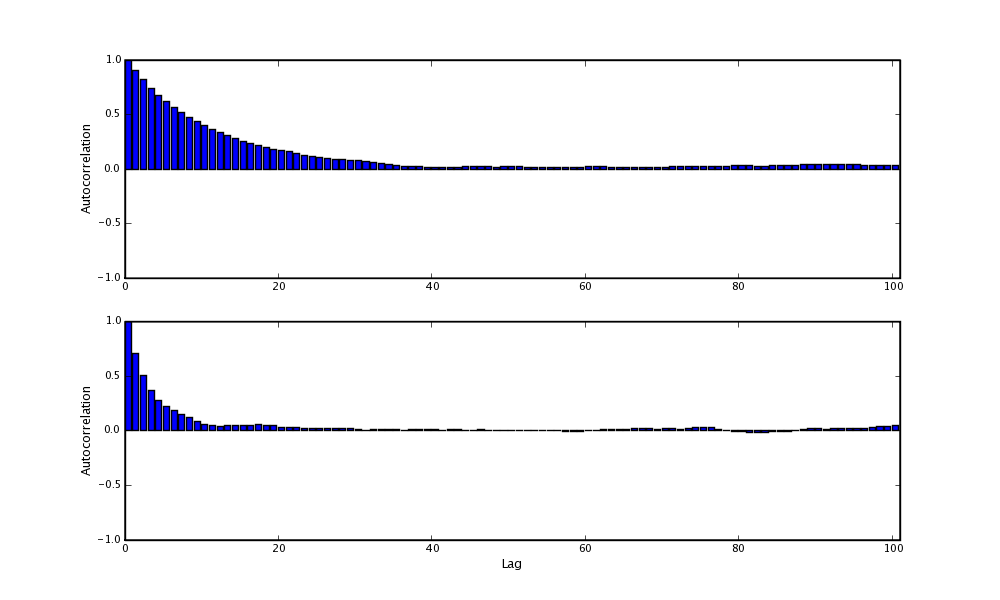
\includegraphics[width=15cm]{autocorr.png}
    \end{center}
    \caption{Sample autocorrelation plots for two Poisson variables from
coal mining disasters example model.}
    \label{fig:autocorr}
\end{figure}

\begin{CodeInput}
autocorrelation(pymc_object, name, maxlag=100, format='png', suffix='-acf',
path='./', fontmap = {1:10, 2:8, 3:6, 4:5, 5:4}, verbose=1)
\end{CodeInput}
\begin{itemize}
  \item \verb=pymc_object=: The object that is or contains the output
trace(s).

  \item \verb=name=: Name used for output files.

  \item \verb=maxlag=: The highest lag interval for which
autocorrelation is calculated.

  \item \verb=format= (optional): Graphic output file format
(defaults to \emph{png}).

  \item \verb=suffix= (optional): Suffix to filename (defaults to
\emph{-diagnostic})

  \item \verb=path= (optional): The path for output graphics
(defaults to working directory).

  \item \verb=fontmap= (optional): Dictionary containing the font map
for the labels of the graphic.

  \item \verb=verbose= (optional): Verbosity level for output
(defaults to 1).
\end{itemize}

Using any given model \code{my_model} as an example, autocorrelation plots can be obtained simply by passing the sampler for that model to the \code{autocorrelation} function (within the \code{Matplot} module) directly:
\begin{CodeInput}
>>> S = pm.MCMC(my_model)
>>> S.sample(10000, burn=5000)
>>> pm.Matplot.autocorrelation(S)
\end{CodeInput}
Alternatively, variables within a model can be plotted individually. For example, a hypothetical variable \code{beta} that was estimated using sampler \code{S} will yield a correlation plot as follows:
\begin{CodeInput}
>>> pm.Matplot.autocorrelation(S.beta)
\end{CodeInput}

\subsection{Goodness of Fit} % (fold)
%\label{sec:goodness_of_fit}

Checking for model convergence is only the first step in the evaluation of MCMC model outputs. It is possible for an entirely unsuitable~model to converge, so additional steps are needed to ensure that the estimated model adequately fits the data. One intuitive way for evaluating model fit is to compare model predictions with actual observations. In other words, the fitted model can be used to simulate data, and the distribution of the simulated data should resemble the distribution of the actual data.

Fortunately, simulating data from the model is a natural component of the Bayesian modelling framework. Recall, from the discussion on imputation of missing data, the posterior predictive distribution:

\begin{equation}
  p(\tilde{y}|y) = \int p(\tilde{y}|\theta) f(\theta|y) d\theta
\end{equation}

Here, $\tilde{y}$ represents some hypothetical new data that would be expected, taking into account the posterior uncertainty in the model parameters. Sampling from the posterior predictive distribution is easy in \pkg{PyMC}. The code looks identical to the corresponding data stochastic, with two modifications: (1) the node should be specified as deterministic and (2) the statistical likelihoods should be replaced by random number generators. As an example, consider a simple dose-response model, where deaths are modeled as a binomial random variable for which the probability of death is a logit-linear function of the dose of a particular drug:
\begin{CodeInput}
n = [5]*4
dose = [-.86,-.3,-.05,.73]
x = [0,1,3,5]

alpha = pm.Normal('alpha', mu=0.0, tau=0.01)
beta = pm.Normal('beta', mu=0.0, tau=0.01)

@pm.deterministic
def theta(a=alpha, b=beta, d=dose):
    """theta = inv_logit(a+b)"""
    return pm.invlogit(a+b*d)

"""deaths ~ binomial(n, p)"""
deaths = pm.Binomial('deaths', n=n, p=theta, value=x, observed=True)
\end{CodeInput}
The posterior predictive distribution of deaths uses the same functional form as the data likelihood, in this case a binomial stochastic. Here is the corresponding sample from the posterior predictive distribution:
\begin{CodeInput}
@pm.deterministic
def deaths_sim(n=n, p=theta):
    """deaths_sim = rbinomial(n, p)"""
    return pm.rbinomial(n, p)
\end{CodeInput}
Notice that the stochastic \code{pm.Binomial} has been replaced with a deterministic node that simulates values using \code{pm.rbinomial} and the unknown parameters \code{theta}. 

The degree to which simulated data correspond to observations can be evaluated in at least two ways. First, these quantities can simply be compared visually. This allows for a qualitative comparison of model-based replicates and observations. If there is poor fit, the true value of the data may appear in the tails of the histogram of replicated data, while a good fit will tend to show the true data in high-probability regions of the posterior predictive distribution (Figure~\ref{fig:gof}).

\begin{figure}[htdevi!]
        \begin{center}
        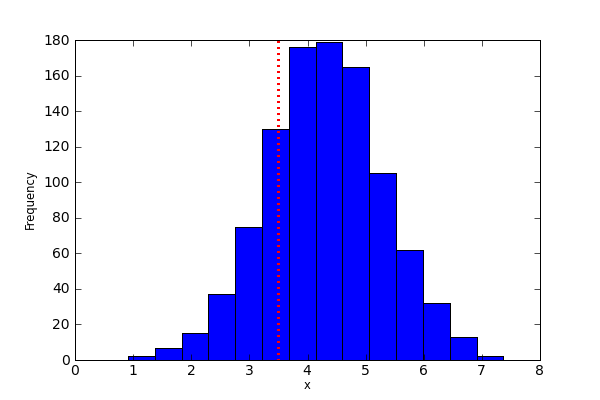
\includegraphics[width=15cm]{gof.png}
    \end{center}
    \caption{Data sampled from the posterior predictive distribution of a model for some observation \textbf{x}. The true value of \textbf{x} is shown by the dotted red line.}
    \label{fig:gof}
\end{figure}

The Matplot module in \pkg{PyMC} provides an easy way of producing such plots, via the \code{gof_plot} function. To illustrate, consider a single observed data point \code{x} and an array of values \code{x_sim} sampled from the posterior predictive distribution. The histogram is generated by calling:

\begin{CodeInput}
pm.Matplot.gof_plot(x_sim, x, name='x')
\end{CodeInput}

A second approach for evaluating goodness of fit using samples from the posterior predictive distribution involves the use of a statistical criterion. For example, the Bayesian p-value \citep{Gelman:1996gp} uses a discrepancy measure that quantifies the difference between data (observed or simulated) $x$ and the expected value $e$, conditional on some model. One such discrepancy measure is the Freeman-Tukey statistic \citep{Brooks:2000il}:

\begin{equation}
  D(x|\theta) = \sum_j (\sqrt{x_j}-\sqrt{e_j})^2
\end{equation}

Model fit is assessed by comparing the discrepancies from observed data to those from simulated data. On average, we expect the difference between them to be zero; hence, the Bayesian p-value is simply the proportion of simulated discrepancies that are larger than their corresponding observed discrepancies:

\begin{equation}
  p = Pr[ D(\text{sim}) > D(\text{obs}) ]
\end{equation}

If $p$ is very large (e.g. $>0.975$) or very small (e.g. $<0.025$) this implies that the model is not consistent with the data, and thus is evidence of lack of fit. Graphically, data and simulated discrepancies plotted together should be clustered along a 45 degree line passing through the origin, as shown in Figure~\ref{fig:deviate}.

\begin{figure}[ht!]
        \begin{center}
        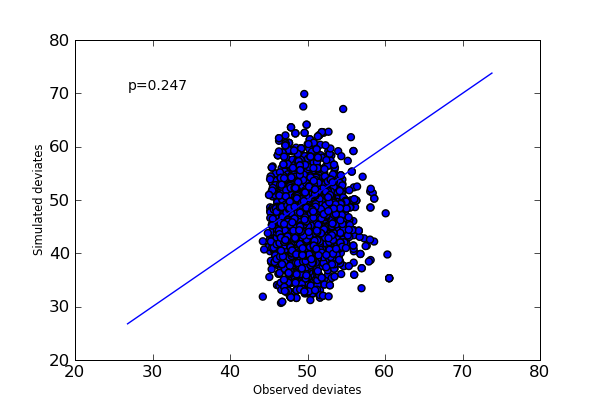
\includegraphics{deviates.png}
    \end{center}
    \caption{Plot of deviates of observed and simulated data from expected values. The cluster of points symmetrically about the 45 degree line (and the reported p-value) suggests acceptable~fit for the modeled parameter.}
    \label{fig:deviate}
\end{figure}
% 
The \code{discrepancy} function in the \code{diagnostics} module can be used to generate discrepancy statistics from arrays of data, simulated values, and expected values:

\begin{CodeInput}
D = pm.diagnostics.discrepancy(x, x_sim, x_exp)
\end{CodeInput}

A call to this function returns two arrays of discrepancy values (one for observed data and one for simulated data), which can be passed to the \code{discrepancy_plot} function in the Matplot module to generate a scatter plot, and if desired, a p-value:

\begin{CodeInput}
pm.Matplot.discrepancy_plot(D, name='D', report_p=True)
\end{CodeInput}

Additional optional arguments for \code{discrepancy_plot} are identical to other \pkg{PyMC} plotting functions.

% Section~goodness_of_fit (end)




\section[Extending PyMC]{Extending \pkg{PyMC}}
\label{chap:extending}
\pkg{PyMC} tries to make standard things easy, but keep unusual things possible. Its openness, combined with \proglang{Python}'s flexibility, invite extensions from using new step methods to exotic stochastic processes (see the Gaussian process module). This Section~briefly reviews the ways \pkg{PyMC} is designed to be extended.


\subsection{Nonstandard Stochastics} \label{nonstandard}


The simplest way to create a \code{Stochastic} object with a nonstandard distribution is to use the medium or long decorator syntax. See Section~\ref{chap:modelbuilding}. If you want to create many stochastics with the same nonstandard distribution, the decorator syntax can become cumbersome. An actual subclass of \code{Stochastic} can be created using the class factory \code{stochastic_from_dist}. This function takes the following arguments:
\begin{itemize}
   \item The name of the new class,
   \item A \code{logp} function,
   \item A \code{random} function (which may be \code{None}),
   \item The \pkg{NumPy} datatype of the new class (for continuous distributions, this should be \code{float}; for discrete distributions, \code{int}; for variables valued as non-numerical objects, \code{object}),
   \item A flag indicating whether the resulting class represents a vector-valued variable.
\end{itemize}
The necessary parent labels are read from the \code{logp} function, and a docstring for the new class is automatically generated.

Full subclasses of \code{Stochastic} may be necessary to provide nonstandard behaviors (see \code{gp.GP}).


\subsection{User-defined step methods} \label{custom-stepper}

The \code{StepMethod} class is meant to be subclassed. There are an enormous number of MCMC step methods in the literature, whereas \pkg{PyMC} provides only about half a dozen. Most user-defined step methods will be either Metropolis-Hastings or Gibbs step methods, and these should subclass \code{Metropolis} or \code{Gibbs} respectively. More unusual step methods should subclass \code{StepMethod} directly.


\subsection{Example: an asymmetric Metropolis step} \label{user-gen}
Consider the probability model in \code{examples/custom_step.py}:
\begin{CodeInput}
mu = pymc.Normal('mu',0,.01, value=0)
tau = pymc.Exponential('tau',.01, value=1)
cutoff = pymc.Exponential('cutoff',1, value=1.3)
D = pymc.TruncatedNormal('D',mu,tau,-numpy.inf,cutoff,value=data,observed=True)
\end{CodeInput}
The stochastic variable \code{cutoff} cannot be smaller than the largest element of $D$, otherwise $D$'s density would be zero. The standard \code{Metropolis} step method can handle this case without problems; it will propose illegal values occasionally, but these will be rejected.

\medskip
Suppose we want to handle \code{cutoff} with a smarter step method that doesn't propose illegal values. Specifically, we want to use the nonsymmetric proposal distribution
\begin{eqnarray*}
  x_p | x \sim \textup{Truncnorm}(x, \sigma, \max(D), \infty).
\end{eqnarray*}
We can implement this Metropolis-Hastings algorithm with the following step method class:
\begin{CodeInput}
class TruncatedMetropolis(pymc.Metropolis):
	def __init__(self, stochastic, low_bound, up_bound, *args, **kwargs):
	    self.low_bound = low_bound
	    self.up_bound = up_bound
	    pymc.Metropolis.__init__(self, stochastic, *args, **kwargs)

	def propose(self):
	    tau = 1./(self.adaptive_scale_factor * self.proposal_sd)**2
	    self.stochastic.value = \
	        pymc.rtruncnorm(self.stochastic.value, tau, self.low_bound, self.up_bound)

	def hastings_factor(self):
	    tau = 1./(self.adaptive_scale_factor * self.proposal_sd)**2
	    cur_val = self.stochastic.value
	    last_val = self.stochastic.last_value

	    lp_for = pymc.truncnorm_like(cur_val, last_val, tau, \
	        self.low_bound, self.up_bound)
	    lp_bak = pymc.truncnorm_like(last_val, cur_val, tau, \
	        self.low_bound, self.up_bound)

	    if self.verbose > 1:
	        print self._id + ': Hastings factor %f'%(lp_bak - lp_for)
	    return lp_bak - lp_for
\end{CodeInput}

The \code{propose} method sets the step method's stochastic's value to a new value, drawn from a truncated normal distribution. The precision of this distribution is computed from two factors: \code{self.proposal_sd}, which can be set with an input argument to Metropolis, and \code{self.adaptive_scale_factor}. Metropolis step methods' default tuning behavior is to reduce \code{adaptive_scale_factor} if the acceptance rate is too low, and to increase \\\code{adaptive_scale_factor} if it is too high. By incorporating \code{adaptive_scale_factor} into the proposal standard deviation, we avoid having to write our own tuning infrastructure. If we don't want the proposal to tune, we don't have to use \code{adaptive_scale_factor}.

The \code{hastings_factor} method adjusts for the asymmetric proposal distribution \citep{gelman}. It computes the log of the quotient of the `backward' density and the `forward' density. For symmetric proposal distributions, this quotient is 1, so its log is zero. 

\medskip
Having created our custom step method, we need to tell MCMC instances to use it to handle the variable \code{cutoff}. This is done in \code{custom_step.py} with the following line:
\begin{CodeInput}
M.use_step_method(TruncatedMetropolis, cutoff, D.value.max(), numpy.inf)
\end{CodeInput}
This call causes $M$ to pass the arguments \code{cutoff, D.value.max(), numpy.inf} to a \\\code{TruncatedMetropolis} object's \code{init} method, and use the object to handle \code{cutoff}.

\medskip
It's often convenient to get a handle to a custom step method instance directly for debugging purposes. \code{M.step_method_dict[cutoff]} returns a list of all the step methods $M$ will use to handle \code{cutoff}:
\begin{CodeInput}
>>> M.step_method_dict[cutoff]
[<custom_step.TruncatedMetropolis object at 0x3c91130>]
\end{CodeInput}
There may be more than one, and conversely step methods may handle more than one stochastic variable. To see which variables step method $S$ is handling, try
\begin{CodeInput}
>>> S.stochastics
set([<pymc.distributions.Exponential 'cutoff' at 0x3cd6b90>])
\end{CodeInput}


\subsection{General step methods} \label{user-gen}


All step methods must implement the following methods:
\begin{description}
   \item[\code{step()}:] Updates the values of \code{self.stochastics}.
   \item[\code{tune()}:] Tunes the jumping strategy based on performance so far. A default method is available that increases \code{self.adaptive_scale_factor} (see below) when acceptance rate is high, and decreases it when acceptance rate is low. This method should return \code{True} if additional tuning will be required later, and \code{False} otherwise.
   \item[\code{competence(s):}] A class method that examines stochastic variable $s$ and returns a value from 0 to 3 expressing the step method's ability to handle the variable. This method is used by \code{MCMC} instances when automatically assigning step methods. Conventions are:
   \begin{description}
      \item[0] I cannot safely handle this variable.
      \item[1] I can handle the variable about as well as the standard \code{Metropolis} step method.
      \item[2] I can do better than \code{Metropolis}.
      \item[3] I am the best step method you are likely to find for this variable in most cases.
   \end{description}
   For example, if you write a step method that can handle \code{NewStochasticSubclass} well, the competence method might look like this:
\begin{CodeInput}
class NewStepMethod(pymc.StepMethod):
    def __init__(self, stochastic, *args, **kwargs):
      ...

    @classmethod
    def competence(self, stochastic):
      if isinstance(stochastic, NewStochasticSubclass):
         return 3
      else:
         return 0
\end{CodeInput}
   Note that \pkg{PyMC} will not even attempt to assign a step method automatically if its \code{init} method cannot be called with a single stochastic instance, that is \code{NewStepMethod(x)} is a legal call. The list of step methods that \pkg{PyMC} will consider assigning automatically is called \code{pymc.StepMethodRegistry}.
   \item[\code{current_state()}:] This method is easiest to explain by showing the code:
   \begin{CodeInput}
state = {}
for s in self._state:
	state[s] = getattr(self, s)
	return state
\end{CodeInput}
   \code{self._state} should be a list containing the names of the attributes needed to reproduce the current jumping strategy. If an \code{MCMC} object writes its state out to a database, these attributes will be preserved. If an \code{MCMC} object restores its state from that database later, the corresponding step method will have these attributes set to their saved values.
\end{description}

Step methods should also maintain the following attributes:
\begin{description}
   \item[\code{_id}:] A string that can identify each step method uniquely (usually something like \\\code{<class_name>_<stochastic_name>}).
   \item[\code{adaptive_scale_factor}:] An `adaptive scale factor'. This attribute is only needed if the default \code{tune()} method is used.
   \item[\code{_tuning_info}:] A list of strings giving the names of any tuning parameters. For \code{Metropolis} instances, this would be \code{[`adaptive_scale_factor']}. This list is used to keep traces of tuning parameters in order to verify `diminishing tuning' \citep{tuning}.
\end{description}

All step methods have a property called \code{loglike}, which gives the sum of the log-probabilities of the union of the extended children of \code{self.stochastics}. This quantity is one term in the log of the Metropolis-Hastings acceptance ratio. The \code{logp_plus_loglike} property gives the sum of that and the log-probabilities of \code{self.stochastics}.  



\subsection{Metropolis-Hastings step methods} \label{user-metro}

A Metropolis-Hastings step method only needs to implement the following methods, which are called by \code{Metropolis.step()}:
\begin{description}
   \item[\code{reject()}:] Usually just
   \begin{CodeInput}
def reject(self):
	self.rejected += 1
	[s.value = s.last_value for s in self.stochastics]
\end{CodeInput}
   \item[\code{propose():}] Sets the values of all \code{self.stochastics} to new, proposed values. This method may use the \code{adaptive_scale_factor} attribute to take advantage of the standard tuning scheme.
\end{description}
Metropolis-Hastings step methods may also override the \code{tune} and \code{competence} methods.

Metropolis-Hastings step methods with asymmetric jumping distributions must implement a method called \code{hastings_factor()}, which returns the log of the ratio of the `reverse' and `forward' proposal probabilities. Note that no \code{accept()} method is needed or used.

Metropolis-Hastings step methods should log the number of jumps they have accepted and rejected using attributes called \code{accepted} and \code{rejected}.


\subsection{Gibbs step methods} \label{user-gibbs}


Gibbs step methods handle conjugate submodels. These models usually have two components: the `parent' and the `children'. For example, a gamma-distributed variable serving as the precision of several normally-distributed variables is a conjugate submodel; the gamma variable is the parent and the normal variables are the children.

This Section~describes \pkg{PyMC}'s current scheme for Gibbs step methods, several of which are in a semi-working state in the \emph{sandbox} directory. It is meant to be as generic as possible to minimize code duplication, but it is admittedly complicated. Feel free to subclass \code{StepMethod} directly when writing Gibbs step methods if you prefer.

Gibbs step methods that subclass \pkg{PyMC}'s \code{Gibbs} should define the following class attributes:
\begin{description}
   \item[\code{child_class}:] The class of the children in the submodels the step method can handle.
   \item[\code{parent_class}:] The class of the parent.
   \item[\code{parent_label}:] The label the children would apply to the parent in a conjugate submodel. In the gamma-normal example, this would be \code{tau}.
   \item[\code{linear_OK}:] A flag indicating whether the children can use linear combinations involving the parent as their actual parent without destroying the conjugacy.
\end{description}

A subclass of \code{Gibbs} that defines these attributes only needs to implement a \code{propose()} method, which will be called by \code{Gibbs.step()}. The resulting step method will be able to handle both conjugate and `non-conjugate' cases. The conjugate case corresponds to an actual conjugate submodel. In the nonconjugate case all the children are of the required class, but the parent is not. In this case the parent's value is proposed from the likelihood and accepted based on its prior. The acceptance rate in the nonconjugate case will be less than one.

The inherited class method \code{Gibbs.competence} will determine the new step method's ability to handle a variable $x$ by checking whether:
\begin{itemize}
   \item all $x$'s children are of class \code{child_class}, and either apply \code{parent_label} to $x$ directly or (if \code{linear_OK=True}) to a \code{LinearCombination} object (Section~\ref{chap:modelbuilding}), one of whose parents contains $x$.
   \item $x$ is of class \code{parent_class}
\end{itemize}
If both conditions are met, \code{pymc.conjugate_Gibbs_competence} will be returned. If only the first is met, \code{pymc.nonconjugate_Gibbs_competence} will be returned.


\subsection{New fitting algorithms} \label{custom-model}


\pkg{PyMC} provides a convenient platform for non-MCMC fitting algorithms in addition to MCMC. All fitting algorithms should be implemented by subclasses of \code{Model}. There are virtually no restrictions on fitting algorithms, but many of \code{Model}'s behaviors may be useful. See Section~\ref{chap:modelfitting}.


\subsection{Monte Carlo fitting algorithms} \label{custom-MC}


Unless there is a good reason to do otherwise, Monte Carlo fitting algorithms should be implemented by subclasses of \code{Sampler} to take advantage of the interactive sampling feature and database backends. Subclasses using the standard \code{sample()} and \code{isample()} methods must define one of two methods:
\begin{description}
   \item[\code{draw()}:] If it is possible to generate an independent sample from the posterior at every iteration, the \code{draw} method should do so. The default \code{_loop} method can be used in this case.
   \item[\code{_loop()}:] If it is not possible to implement a \code{draw()} method, but you want to take advantage of the interactive sampling option, you should override \code{_loop()}. This method is responsible for generating the posterior samples and calling \code{tally()} when it is appropriate to save the model's state. In addition, \code{_loop} should monitor the sampler's \code{status} attribute at every iteration and respond appropriately. The possible values of \code{status} are:
   \begin{description}
      \item[\code{`ready'}:] Ready to sample.
      \item[\code{`running'}:] Sampling should continue as normal.
      \item[\code{`halt'}:] Sampling should halt as soon as possible. \code{_loop} should call the \code{halt()} method and return control. \code{_loop} can set the status to \code{`halt'} itself if appropriate (eg the database is full or a \code{KeyboardInterrupt} has been caught).
      \item[\code{`paused'}:] Sampling should pause as soon as possible. \code{_loop} should return, but should be able to pick up where it left off next time it's called.
   \end{description}
\end{description}

Samplers may alternatively want to override the default \code{sample()} method. In that case, they should call the \code{tally()} method whenever it is appropriate to save the current model state. Like custom \code{_loop()} methods, custom \code{sample()} methods should handle \code{KeyboardInterrupts} and call the \code{halt()} method when sampling terminates to finalize the traces.


\subsection{A second warning: Don't update stochastic variables' values in-place}
\label{dont-update-indepth}


If you're going to implement a new step method, fitting algorithm or unusual (non-numeric-valued) \code{Stochastic} subclass, you should understand the issues related to in-place updates of \code{Stochastic} objects' values. Fitting methods should never update variables' values in-place for two reasons:
\begin{itemize}
   \item In algorithms that involve accepting and rejecting proposals, the `pre-proposal' value needs to be preserved uncorrupted. It would be possible to make a copy of the pre-proposal value and then allow in-place updates, but in \pkg{PyMC} we have chosen to store the pre-proposal value as \code{Stochastic.last_value} and require proposed values to be new objects. In-place updates would corrupt \code{Stochastic.last_value}, and this would cause problems.
   \item \code{LazyFunction}'s caching scheme checks variables' current values against its internal cache by reference. That means if you update a variable's value in-place, it or its child may miss the update and incorrectly skip recomputing its value or log-probability.
\end{itemize}

However, a \code{Stochastic} object's value can make in-place updates to itself if the updates don't change its identity. For example, the \code{Stochastic} subclass \code{gp.GP} is valued as a \code{gp.Realization} object. These represent random functions, which are infinite-dimensional stochastic processes, as literally as possible. The strategy they employ is to `self-discover' on demand: when they are evaluated, they generate the required value conditional on previous evaluations and then make an internal note of it. This is an in-place update, but it is done to provide the same interface as a single random function whose value everywhere has been determined since it was created.


\clearpage

\section{Conclusion}
\label{conclusion}

MCMC is a surprisingly difficult and bug-prone algorithm to implement by hand. We find \pkg{PyMC} makes it much easier and less stressful. \pkg{PyMC} also makes our work more dynamic; getting hand-coded MCMC's working used to be so much work that we were reluctant to change anything, but with \pkg{PyMC} changing models is much easier. 

We welcome new contributors at all levels. If you would like to contribute new code, improve documentation, share your results or provide ideas for new features, please introduce yourself on our mailing list at \href{pymc@googlegroups.com}{pymc@googlegroups.com}. Our wiki page at \href{http://code.google.com/p/pymc/w/list}{http://code.google.com/p/ pymc/w/list} also hosts a number of tutorials and examples from users that could give you some ideas. We have taken great care to make the code easy to extend, whether by adding new database backends, step methods or entirely new sampling algorithms.





\section[Acknowledgments]{Acknowledgments}
\label{chap:acknowledge}
The authors would like to thank several users of \pkg{PyMC} who have been particularly helpful during the development of the 2.0 release. In alphabetical order, these are Mike Conroy, Abraham Flaxman, J. Miguel Marin, Aaron MacNeil, Nick Matsakis, John Salvatier and Andrew Straw.

Anand Patil's work on \pkg{PyMC} has been supported since 2008 by the Malaria Atlas Project, principally funded by the Wellcome Trust.

David Huard's early work on \pkg{PyMC} was supported by a scholarship from the Natural Sciences and Engineering Research Council of Canada. 
\newpage
\appendix

% \section[Distributions]{Probability distributions}



\pkg{PyMC} provides 35 built-in probability distributions. For each distribution, \pkg{PyMC} provides:
\begin{itemize}
    \item A function that evaluates its log-probability or log-density, for example \code{normal_like()}.
    \item A function that draws random variables, for example \code{rnormal()}.
    \item A function that computes the expectation associated with the distribution, for example \code{normal_expval()}.
    \item A \code{Stochastic} subclass generated from the distribution, for example \code{Normal}.
\end{itemize}

This Section~describes the likelihood functions of these distributions.

\section{Discrete distributions}
%\label{chap:discrete} 

\subsection[bernoulli]{\code{bernoulli_like(x, p)}}
     
The Bernoulli distribution describes the probability of successes $(x=1)$ and
failures $(x=0)$.
\begin{eqnarray*}
    f(x \mid p) = p^{x} (1-p)^{1-x}
\end{eqnarray*}

\begin{description}
\item[Parameters] \ 

\begin{itemize}
\item {} 
\emph{x} : Series of successes (1) and failures (0). $x=0,1$

\item {} 
\emph{p} : Probability of success, $p \in [0,1]$.
\end{itemize}
\item[Notes] \ 
\begin{itemize}
\item {} 
$\E(x)= p$
\item {} 
$\VAR(x)= p(1-p)$
\end{itemize}
\end{description}


\subsection[binomial]{\code{binomial_like(x, n, p)}}

Binomial log-likelihood.  The discrete probability distribution of the
number of successes in a sequence of n independent yes/no experiments,
each of which yields success with probability $p$.
\begin{eqnarray*}
f(x \mid n, p) = \frac{n!}{x!(n-x)!} p^x (1-p)^{n-x}    
\end{eqnarray*}
\begin{description}
\item[Parameters] \ 

\begin{itemize}
\item {} 
\emph{x} : {[}int{]} Number of successes, \textgreater{} 0.

\item {} 
\emph{n} : {[}int{]} Number of Bernoulli trials, \textgreater{} x.

\item {} 
\emph{p} : Probability of success in each trial, $p \in [0,1]$.

\end{itemize}

\item[Notes] \ 

\begin{itemize}
\item {} 
$\E(X)=np$

\item {} 
$\VAR(X)=np(1-p)$

\end{itemize}


\end{description}




\subsection[categorical]{\code{categorical_like(x, p)} }

Categorical log-likelihood. The most general discrete distribution.
\begin{eqnarray*}
f(x=i \mid p) = p_i    
\end{eqnarray*}
for $i \in 0 \ldots k-1$.
\begin{description}
\item[Parameters] \ 

\begin{itemize}
\item {} 
\emph{x} : {[}int{]} $x \in 0\ldots k-1$

\item {} 
\emph{p} : {[}float{]} $p > 0$, $\sum p = 1$

\end{itemize}

\end{description}


\subsection[discrete uniform]{\code{discrete_uniform_like(x, lower, upper)}}

Discrete uniform log-likelihood.
\begin{eqnarray*}
f(x \mid lower, upper) = \frac{1}{upper-lower}    
\end{eqnarray*}

\begin{description} 
\item[Parameters] \leavevmode\begin{itemize}
\item {} 
\emph{x} : {[}int{]} $lower \leq x \leq upper$

\item {} 
\emph{lower} : Lower limit.

\item {} 
\emph{upper} : Upper limit (\emph{upper} \textgreater{} \emph{lower}).

\end{itemize}

\end{description}

\subsection[geometric]{\code{geometric_like(x, p)}} 

Geometric log-likelihood. The probability that the first success in a
sequence of Bernoulli trials occurs on the $x$'th trial.
\begin{eqnarray*}
f(x \mid p) = p(1-p)^{x-1}    
\end{eqnarray*}
\begin{description}
\item[Parameters] \leavevmode\begin{itemize}
\item {} 
\emph{x} : {[}int{]} Number of trials before first success, \textgreater{} 0.

\item {} 
\emph{p} : Probability of success on an individual trial, $p \in [0,1]$

\end{itemize}

\item[Notes] \leavevmode\begin{itemize}
\item {} 
$\E(X)=1/p$

\item {} 
$\VAR(X)=\frac{1-p}{p^2}$
\end{itemize}

\end{description}

\subsection[hypergeometric]{\code{hypergeometric_like(x, n, m, N)}} 

Hypergeometric log-likelihood. Discrete probability distribution that
describes the number of successes in a sequence of draws from a finite
population without replacement.
\begin{eqnarray*}
f(x \mid n, m, N) = \frac{\binom{m}{x}\binom{N-m}{n-x}}{\binom{N}{n}}
\end{eqnarray*}
\begin{description}    
\item[Parameters] \leavevmode\begin{itemize}
\item {} 
\emph{x} : {[}int{]} Number of successes in a sample drawn from a population.

\item {} 
\emph{n} : {[}int{]} Size of sample drawn from the population.

\item {} 
\emph{m} : {[}int{]} Number of successes in the population.

\item {} 
\emph{N} : {[}int{]} Total number of units in the population.

\end{itemize}

\item[Notes] \leavevmode\begin{itemize}
\item $\E(X) = \frac{n m}{N}$
\end{itemize}

\end{description}


\subsection[negative binomial]{\code{negative_binomial_like(x, mu, alpha)}}

Negative binomial log-likelihood. The negative binomial distribution describes a
Poisson random variable whose rate parameter is gamma distributed. \pkg{PyMC}'s chosen
parameterization is based on this mixture interpretation.

\begin{eqnarray*}
f(x \mid \mu, \alpha) = \frac{\Gamma(x+\alpha)}{x! \Gamma(\alpha)} (\alpha/(\mu+\alpha))^\alpha (\mu/(\mu+\alpha))^x    
\end{eqnarray*}

\begin{description}
\item[Parameters] \leavevmode\begin{itemize}
\item {} 
\emph{x} : Input data, \textgreater{} 0.

\item {} 
\emph{mu} : \textgreater{} 0

\item {} 
\emph{alpha} : \textgreater{} 0

\end{itemize}

\item[Notes]\leavevmode\begin{itemize}
\item {} 
$\E[x]=\mu$

\item {} 
In Wikipedia's parameterization,
$r=\alpha$
$p=\alpha/(\mu+\alpha)$
$\mu=r(1-p)/p$

\end{itemize}


\end{description}

\subsection[Poisson]{\code{poisson_like(x, mu)}}

Poisson log-likelihood. The Poisson is a discrete probability distribution.
It is often used to model the number of events occurring in a fixed period of
time when the times at which events occur are independent. The Poisson
distribution can be derived as a limiting case of the binomial distribution.

\begin{eqnarray*}
    f(x \mid \mu) = \frac{e^{-\mu}\mu^x}{x!}
\end{eqnarray*}

\begin{description}
\item[Parameters] \leavevmode\begin{itemize}
\item {} 
\emph{x} : {[}int{]} $x \in {0,1,2,...}$

\item {} 
\emph{mu} : Expected number of occurrences during the given interval, $\geq 0$.

\end{itemize}

\item[Notes]\leavevmode\begin{itemize}
\item {} 
$\E(x)=\mu$

\item {} 
$\VAR(x)=\mu$

\end{itemize}

\end{description}



\section{Continuous distributions}
%\label{chap:continuous} 


\subsection[beta]{\code{beta_like(x, alpha, beta)} }

Beta log-likelihood. The conjugate prior for the parameter \emph{p} of the binomial distribution.

\begin{eqnarray*}
    f(x \mid \alpha, \beta) = \frac{\Gamma(\alpha + \beta)}{\Gamma(\alpha) \Gamma(\beta)} x^{\alpha - 1} (1 - x)^{\beta - 1}
\end{eqnarray*}

\begin{description}
\item[Parameters] \leavevmode\begin{itemize}
\item {} 
\emph{x} : 0 \textless{} \emph{x} \textless{} 1

\item {} 
\emph{alpha} : \textgreater{} 0

\item {} 
\emph{beta} : \textgreater{} 0

\end{itemize}


\item[Notes]\leavevmode\begin{itemize}
\item {} 
$\E(X)=\frac{\alpha}{\alpha+\beta}$

\item {} 
$\VAR(X)=\frac{\alpha \beta}{(\alpha+\beta)^2(\alpha+\beta+1)}$

\end{itemize}

\end{description}


\subsection[Cauchy]{\code{cauchy_like(x, alpha, beta)}}


Cauchy log-likelihood. The Cauchy distribution is also known as the
Lorentz or the Breit-Wigner distribution.

\begin{eqnarray*}
f(x \mid \alpha, \beta) = \frac{1}{\pi \beta [1 + (\frac{x-\alpha}{\beta})^2]}    
\end{eqnarray*}

\begin{description}
\item[Parameters] \leavevmode\begin{itemize}
\item {} 
\emph{alpha} : Location parameter.

\item {} 
\emph{beta} : Scale parameter, \textgreater{} 0.

\end{itemize}

\item[Notes]\leavevmode\begin{itemize}
\item {} 
Mode and median are at alpha.

\end{itemize}

\end{description}

\subsection[chi2]{\code{chi2_like(x, nu)} }

$\chi^2$ log-likelihood.
\begin{eqnarray*}
    f(x \mid \nu) = \frac{x^{(\nu-2)/2}e^{-x/2}}{2^{\nu/2}\Gamma(\nu/2)}
\end{eqnarray*}

\begin{description}
\item[Parameters] \leavevmode\begin{itemize}
\item {} 
\emph{x} : \textgreater{} 0

\item {} 
\emph{nu} : {[}int{]} Degrees of freedom, \textgreater{} 0

\end{itemize}

\item[Notes]\leavevmode\begin{itemize}
\item {} 
$\E(X)=\nu$

\item {} 
$\VAR(X)=2\nu$

\end{itemize}


\end{description}

\subsection[degenerate]{\code{degenerate_like(x, k)}}

Degenerate log-likelihood.

\begin{eqnarray*}
f(x \mid k) = \left\{ \begin{matrix} 1 \text{ if } x = k \\ 0 \text{ if } x \ne k\end{matrix} \right.    
\end{eqnarray*}

\begin{description}
\item[Parameters] \leavevmode\begin{itemize}
\item {} 
\emph{x} : Input value.

\item {} 
\emph{k} : Degenerate value.

\end{itemize}

\end{description}


\subsection[exponential]{\code{exponential_like(x, beta)} }

Exponential log-likelihood.

The exponential distribution is a special case of the gamma distribution
with $\alpha=1$. It often describes the time until an event.
\begin{eqnarray*}
f(x \mid \beta) = \frac{1}{\beta}e^{-x/\beta}    
\end{eqnarray*}

\begin{description}
\item[Parameters] \leavevmode\begin{itemize}
\item {} 
\emph{x} : \textgreater{} 0

\item {} 
\emph{beta} : Survival parameter, \textgreater{} 0.

\end{itemize}

\item[Notes]\leavevmode\begin{itemize}
\item {} 
$\E(X) = \beta$

\item {} 
$\VAR(X) = \beta^2$

\end{itemize}

\end{description}

\subsection[exponentiated Weibull]{\code{exponweib(x, alpha, k, loc, scale)} }

Exponentiated Weibull log-likelihood.

The exponentiated Weibull distribution is a generalization of the Weibull
family. Its value lies in being able to model monotone and non-monotone
failure rates.
\begin{align*}
    f(x \mid \alpha,k,loc,scale)  & = \frac{\alpha k}{scale} (1-e^{-z^k})^{\alpha-1} e^{-z^k} z^{k-1} \\
    z & = \frac{x-loc}{scale}    
\end{align*}
\begin{description}
\item[Parameters] \leavevmode\begin{itemize}
\item {} 
\emph{x} : \textgreater{} 0

\item {} 
\emph{alpha} : Shape parameter

\item {} 
\emph{k} : \textgreater{} 0

\item {} 
\emph{loc} : Location parameter

\item {} 
\emph{scale} : Scale parameter, \textgreater{} 0.

\end{itemize}

\end{description}

\subsection[gamma]{\code{gamma_like(x, alpha, beta)} }

Gamma log-likelihood.

Represents the sum of alpha exponentially distributed random variables, each
of which has mean beta.
\begin{eqnarray*}
f(x \mid \alpha, \beta) = \frac{\beta^{\alpha}x^{\alpha-1}e^{-\beta x}}{\Gamma(\alpha)}    
\end{eqnarray*}
\begin{description}
\item[Parameters] \leavevmode\begin{itemize}
\item {} 
\emph{x} : $\ge 0$

\item {} 
\emph{alpha} : Shape parameter, \textgreater{} 0.

\item {} 
\emph{beta} : Scale parameter, \textgreater{} 0.

\end{itemize}

\item[Notes]\leavevmode\begin{itemize}
\item {} 
$\E(X) = \frac{\alpha}{\beta}$

\item {} 
$\VAR(X) = \frac{\alpha}{\beta^2}$

\end{itemize}

\end{description}

\subsection[half normal]{\code{half_normal_like(x, tau)} }

Half-normal log-likelihood, a normal distribution with mean 0 limited
to the domain $[0, \infty)$.
\begin{eqnarray*}
f(x \mid \tau) = \sqrt{\frac{2\tau}{\pi}}\exp\left\{ {\frac{-x^2 \tau}{2}}\right\}    
\end{eqnarray*}
\begin{description}
\item[Parameters] \leavevmode\begin{itemize}
\item {} 
\emph{x} : $\ge 0$

\item {} 
\emph{tau} : \textgreater{} 0

\end{itemize}

\end{description}


\subsection[inverse gamma]{\code{inverse_gamma_like(x, alpha, beta)} }

Inverse gamma log-likelihood, the reciprocal of the gamma distribution.

\begin{eqnarray*}
f(x \mid \alpha, \beta) = \frac{\beta^{\alpha}}{\Gamma(\alpha)} x^{-\alpha - 1} \exp\left(\frac{-\beta}{x}\right)    
\end{eqnarray*}

\begin{description}
\item[Parameters] \leavevmode\begin{itemize}
\item {} 
\emph{x} : \textgreater{} 0

\item {} 
\emph{alpha} : Shape parameter, \textgreater{} 0.

\item {} 
\emph{beta} : Scale parameter, \textgreater{} 0.

\end{itemize}

\item[Notes]\leavevmode \begin{itemize} 
\item {}
$\E(X)=\frac{\beta}{\alpha-1}$  for $\alpha > 1$

\item {}
$\VAR(X)=\frac{\beta^2}{(\alpha-1)^2(\alpha)}$  for $\alpha > 2$
\end{itemize} 


\end{description}



\subsection[Laplace]{\code{laplace_like(x, mu, tau)} }
Laplace (double exponential) log-likelihood.

The Laplace (or double exponential) distribution describes the
difference between two independent, identically distributed exponential
events. It is often used as a heavier-tailed alternative to the normal.

\begin{eqnarray*}
f(x \mid \mu, \tau) = \frac{\tau}{2}e^{-\tau |x-\mu|}    
\end{eqnarray*}

\begin{description}
\item[Parameters] \leavevmode\begin{itemize}

\item {} 
\emph{mu} : Location parameter

\item {} 
\emph{tau} : Precision parameter, $> 0$

\end{itemize}

\item[Notes]\leavevmode\begin{itemize}
\item {} 
$\E(X) = \mu$

\item {} 
$\VAR(X) = \frac{2}{\tau^2}$

\end{itemize}


\end{description}


\subsection[logistic]{\code{logistic_like(x, mu, tau)}}

Logistic log-likelihood.

The logistic distribution is often used as a growth model; for example,
populations, markets. Resembles a heavy-tailed normal distribution.
\begin{eqnarray*}
f(x \mid \mu, \tau) = \frac{\tau \exp(-\tau[x-\mu])}{[1 + \exp(-\tau[x-\mu])]^2}    
\end{eqnarray*}

\begin{description}
\item[Parameters] \leavevmode\begin{itemize}

\item {} 
\emph{mu} : Location parameter

\item {} 
\emph{tau} : Precision parameter, \textgreater{} 0

\end{itemize}

\item[Notes]\begin{itemize}
\item {} 
$\E(X) = \mu$

\item {} 
$\VAR(X) = \frac{\pi^2}{3\tau^2}$

\end{itemize}

\end{description}


\subsection[lognormal]{\code{lognormal_like(x, mu, tau)}}

Log-normal log-likelihood. Distribution of any random variable whose
logarithm is normally distributed. A variable might be modeled as
log-normal if it can be thought of as the multiplicative product of many
small independent factors.

\begin{eqnarray*}
    f(x \mid \mu, \tau) = \sqrt{\frac{\tau}{2\pi}}\frac{
    \exp\left\{ -\frac{\tau}{2} (\ln(x)-\mu)^2 \right\}}{x}    
\end{eqnarray*}

\begin{description}
\item[Parameters] \leavevmode\begin{itemize}

\item {} 
\emph{mu} : Location parameter

\item {} 
\emph{tau} : Precision parameter, \textgreater{} 0

\end{itemize}

\item[Notes] \leavevmode\begin{itemize}
    \item {}
    $\E(X)=e^{\mu+\frac{1}{2\tau}}$
    
    \item {}
    $\VAR(X)=(e^{1/\tau}-1)e^{2\mu+\frac{1}{\tau}}$
\end{itemize}

\end{description}


\subsection[normal]{\code{normal_like(x, mu, tau)}}

Normal log-likelihood.
\begin{eqnarray*}
    f(x \mid \mu, \tau) = \sqrt{\frac{\tau}{2\pi}} \exp\left\{ -\frac{\tau}{2} (x-\mu)^2 \right\}
\end{eqnarray*}

\begin{description}
\item[Parameters] \leavevmode\begin{itemize}

\item {} 
\emph{mu} : Location parameter

\item {} 
\emph{tau} : Precision parameter, \textgreater{} 0.

\end{itemize}

\item[Notes]\leavevmode\begin{itemize}
\item {} 
$\E(X) = \mu$

\item {} 
$\VAR(X) = 1/\tau$

\end{itemize}

\end{description}


\subsection[skew normal]{\code{skew_normal_like(x, mu, tau, alpha)} }

Azzalini's skew-normal log-likelihood
\begin{eqnarray*}
f(x \mid \mu, \tau, \alpha) = 2 \Phi((x-\mu)\sqrt{\tau}\alpha) \phi(x,\mu,\tau)    
\end{eqnarray*}

where $\Phi$ is the normal CDF and $\phi$ is the normal PDF.

\begin{description}
\item[Parameters] \leavevmode\begin{itemize}


\item {} 
\emph{mu} : Location parameter

\item {} 
\emph{tau} : Precision parameter, \textgreater{} 0

\item {} 
\emph{alpha} : Shape parameter

\end{itemize}

\item[Notes]\leavevmode
\begin{itemize}
    \item {}
    See \href{http://azzalini.stat.unipd.it/SN/}{http://azzalini.stat.unipd.it/SN/}
\end{itemize}

\end{description}

\subsection[Student's T]{\code{t_like(x, nu)} }

Student's T log-likelihood. Describes a zero-mean normal variable whose precision is
gamma distributed. Alternatively, describes the mean of several zero-mean normal
random variables divided by their sample standard deviation.

\begin{eqnarray*}
f(x \mid \nu) = \frac{\Gamma(\frac{\nu+1}{2})}{\Gamma(\frac{\nu}{2}) \sqrt{\nu\pi}} \left( 1 + \frac{x^2}{\nu} \right)^{-\frac{\nu+1}{2}}    
\end{eqnarray*}

\begin{description}
\item[Parameters] \leavevmode\begin{itemize}

\item {} 
\emph{nu} : Degrees of freedom

\end{itemize}

\end{description}

\subsection[truncated normal]{\code{truncnorm_like(x, mu, tau, a, b)} }

Truncated normal log-likelihood.
\begin{eqnarray*}
f(x \mid \mu, \tau, a, b) = \frac{\phi(\frac{x-\mu}{\sigma})} {\Phi(\frac{b-\mu}{\sigma}) - \Phi(\frac{a-\mu}{\sigma})}    
\end{eqnarray*}

where $\sigma^2=1/\tau$, $\phi$ is the standard normal PDF and $\Phi$ is the standard normal CDF.
\begin{description}
\item[Parameters] \leavevmode\begin{itemize}

\item {} 
\emph{mu} : Location parameter

\item {} 
\emph{tau} : Precision parameter

\item {} 
\emph{a} : Lower limit

\item {} 
\emph{b} : Upper limit

\end{itemize}

\end{description}

\subsection[uniform]{\code{uniform_like(x, lower, upper)} }


Uniform log-likelihood.
\begin{eqnarray*}
f(x \mid lower, upper) = \frac{1}{upper-lower}    
\end{eqnarray*}

\begin{description}
\item[Parameters] \leavevmode\begin{itemize}
\item {} 
\emph{x} : $lower \leq x \leq upper$

\item {} 
\emph{lower} : Lower limit

\item {} 
\emph{upper} : Upper limit, (\emph{upper} \textgreater{} \emph{lower})

\end{itemize}

\end{description}

\subsection[von Mises]{\code{von_mises_like(x, mu, kappa)} }

von Mises log-likelihood.
\begin{eqnarray*}
f(x \mid \mu, k) = \frac{e^{k \cos(x - \mu)}}{2 \pi I_0(k)}    
\end{eqnarray*}
where $I_0$ is the modified Bessel function of order 0.
\begin{description}
\item[Parameters] \leavevmode\begin{itemize}

\item {} 
\emph{mu} : Location parameter

\item {} 
\emph{kappa} : Dispersion parameter

\end{itemize}

\item[Notes]\leavevmode\begin{itemize}
\item {} 
$\E(X) = \mu$

\end{itemize}


\end{description}

\subsection[Weibull]{\code{weibull_like(x, alpha, beta)} }


Weibull log-likelihood
\begin{eqnarray*}
    f(x \mid \alpha, \beta) = \frac{\alpha x^{\alpha - 1}
    \exp(-(\frac{x}{\beta})^{\alpha})}{\beta^\alpha}    
\end{eqnarray*}
\begin{description}
\item[Parameters] \leavevmode\begin{itemize}
\item {} 
\emph{x} : $\ge 0$

\item {} 
\emph{alpha} : \textgreater{} 0

\item {} 
\emph{beta} : \textgreater{} 0

\end{itemize}

\item[Notes]\leavevmode\begin{itemize}
\item {} 
$\E(x)=\beta \Gamma(1+\frac{1}{\alpha})$

\item {} 
$\VAR(x)=\beta^2 \Gamma(1+\frac{2}{\alpha} - \mu^2)$

\end{itemize}

\end{description}


\section{Multivariate discrete distributions} % (fold)
%\label{chap:multivariate_discrete}

\subsection[multivariate hypergeometric]{\code{multivariate_hypergeometric_like(x, mu, m)} }


The multivariate hypergeometric describes the probability of drawing $x_i$
elements of the $i$th category, when the number of items in each category is
given by $m$.
\begin{eqnarray*}
\frac{\prod_i \binom{m_i}{x_i}}{\binom{N}{n}}    
\end{eqnarray*}

where $N = \sum_i m_i$ and $n = \sum_i x_i$.
\begin{description}
\item[Parameters] \leavevmode\begin{itemize}
\item {} 
\emph{x} : {[}int sequence{]} Number of draws from each category, $x$ \textless{} $m$

\item {} 
\emph{m} : {[}int sequence{]} Number of items in each category

\end{itemize}

\end{description}

\subsection[multinomial]{\code{multinomial_like(x, n, p)} }

Multinomial log-likelihood. Generalization of the binomial
distribution, but instead of each trial resulting in ``success'' or
``failure'', each one results in exactly one of some fixed finite number $k$
of possible outcomes over n independent trials. $x_i$ indicates the number
of times outcome number $i$ was observed over the $n$ trials.

\begin{eqnarray*}
f(x \mid n, p) = \frac{n!}{\prod_{i=1}^k x_i!} \prod_{i=1}^k p_i^{x_i}    
\end{eqnarray*}
    
\begin{description}
\item[Parameters] \leavevmode\begin{itemize}
\item{} 

\emph{x} : {[}$(k)$ int{]} Random variable indicating the number of time outcome $i$ is 
observed, $\sum_{i=1}^k x_i=n$, $x_i \ge 0$

\item{} 
\emph{n} : {[}int{]}
Number of trials

\item {}
\emph{p} : {[}$(k)$ {]} Probability of each one of the different outcomes,
$\sum_{i=1}^k p_i = 1$, $p_i \ge 0$



\end{itemize}

\item[Notes]\leavevmode\begin{itemize}
\item {} 
$\E(X_i)=n p_i$

\item {} 
$\VAR(X_i)=n p_i(1-p_i)$

\item {} 
$\COV(X_i,X_j) = -n p_i p_j$

\end{itemize}

\end{description}


% section multivariate_discrete_distributions (end)

\section{Multivariate continuous distributions} % (fold)
%\label{chap:multivariate_continuous}

\subsection[Dirichlet]{\code{dirichlet_like(x, theta)} }


Dirichlet log-likelihood.

This is a multivariate continuous distribution.
\begin{eqnarray*}
f(x) = \frac{\Gamma(\sum_{i=1}^k \theta_i)}{\prod \Gamma(\theta_i)}\prod_{i=1}^{k-1} x_i^{\theta_i - 1}\cdot\left(1-\sum_{i=1}^{k-1}x_i\right)^{\theta_k}    
\end{eqnarray*}
\begin{description}
\item[Parameters] \leavevmode\begin{itemize}
\item{}
\emph{x} : {[}$(k-1)$ {]}, $0 < x_i < 1$,  $\sum_{i=1}^{k-1} x_i < 1$
\item{}
$\theta$ : \leavevmode{[}$(k)$ {]}, $\theta_i> 0$

\end{itemize}

\item[Notes]\leavevmode \begin{itemize}
    \item {}
    Only the first \emph{k-1} elements of \emph{x} are expected. Can be used as a parent of Multinomial and Categorical
    nevertheless.    
\end{itemize}

\end{description}


\subsection[inverse Wishart]{\code{inverse_wishart_like(x, n, Tau)} }

Inverse Wishart log-likelihood. The inverse Wishart distribution is the conjugate
prior for the covariance matrix of a multivariate normal distribution.
\begin{eqnarray*}
f(x \mid n, T) = \frac{{\mid T \mid}^{n/2}{\mid x \mid}^{(n-k-1)/2} \exp\left\{ -\frac{1}{2} Tr(Tx^{-1}) \right\}}{2^{nk/2} \Gamma_p(n/2)}    
\end{eqnarray*}

where $k$ is the rank of $x$.
\begin{description}
\item[Parameters] \leavevmode\begin{itemize}
\item {} 
\emph{x} : Symmetric, positive definite matrix

\item {} 
\emph{n} : {[}int{]} Degrees of freedom, \textgreater{} 0

\item {} 
\emph{Tau} : Symmetric and positive definite matrix

\end{itemize}

\item[Notes]\leavevmode
\begin{itemize}
    \item {}
    Step method MatrixMetropolis will preserve the symmetry of Wishart variables.
\end{itemize}

\end{description}


\subsection[multivariate normal]{\code{mv_normal_like(x, mu, Tau)}}

Multivariate normal log-likelihood
\begin{eqnarray*}
f(x \mid \pi, T) = \frac{|T|^{1/2}}{(2\pi)^{1/2}} \exp\left\{ -\frac{1}{2} (x-\mu)^{\prime}T(x-\mu) \right\}    
\end{eqnarray*}

\begin{description}
\item[Parameters] \leavevmode\begin{itemize}

\item {} 
\emph{mu} : [$(k)$] Location parameter sequence

\item {} 
\emph{Tau} : [$(k,k)$] Positive definite precision matrix

\end{itemize}

\end{description}


\subsection[multivariate normal, Cholesky parameterization]{\code{mv_normal_chol_like(x, mu, sigma)} }

Multivariate normal log-likelihood.
\begin{eqnarray*}
f(x \mid \pi, \sigma) = \frac{1}{(2\pi)^{1/2}|\sigma|)} \exp\left\{ -\frac{1}{2} (x-\mu)^{\prime}(\sigma \sigma^{\prime})^{-1}(x-\mu) \right\}    
\end{eqnarray*}

\begin{description}
\item[Parameters] \leavevmode\begin{itemize}
\item {} 
\emph{x} : [$(k)$]

\item {} 
\emph{mu} : [$(k)$] Location parameter

\item {} 
\emph{sigma} : [$(k,k)$] Lower triangular Cholesky factor of covariance matrix

\end{itemize}

\end{description}


\subsection[multivariate normal, covariance parameterization]{\code{mv_normal_cov_like(x, mu, C)} }

Multivariate normal log-likelihood parameterized by a covariance matrix.
\begin{eqnarray*}
f(x \mid \pi, C) = \frac{1}{(2\pi|C|)^{1/2}} \exp\left\{ -\frac{1}{2} (x-\mu)^{\prime}C^{-1}(x-\mu) \right\}    
\end{eqnarray*}
\begin{description}
\item[Parameters] \leavevmode\begin{itemize}
\item {} 
\emph{x} : [$(k)$]

\item {} 
\emph{mu} : [$(k)$] Location parameter

\item {} 
\emph{C} : [$(k,k)$] Positive definite covariance matrix

\end{itemize}

\end{description}


\subsection[Wishart]{\code{wishart_like(x, n, Tau)} }

Wishart log-likelihood. The Wishart distribution is the probability
distribution of the maximum-likelihood estimator (MLE) of the precision
matrix of a multivariate normal distribution.

For an alternative parameterization based on $C=T^{-1}$, see
\code{wishart\_cov\_like}.
\begin{eqnarray*}
f(x \mid n, T) = {\mid T \mid}^{n/2}{\mid X \mid}^{(n-k-1)/2} \exp\left\{ -\frac{1}{2} Tr(Tx) \right\}    
\end{eqnarray*}
where $k$ is the rank of $x$.
\begin{description}
\item[Parameters] \leavevmode\begin{itemize}
\item {} 
\emph{x} : [$(k,k)$] Positive definite

\item{} 
\emph{n} : [int] Degrees of freedom, \textgreater{} 0

\item{}
\emph{Tau} : [$(k,k)$] Positive definite

\end{itemize}

\item[Notes]\leavevmode
\begin{itemize}
    \item {}
    Step method MatrixMetropolis will preserve the symmetry of Wishart variables.
\end{itemize}

\end{description}



\subsection[Wishart, covariance parameterization]{\code{wishart_cov_like(x, n, C)} }

Wishart log-likelihood. The Wishart distribution is the probability
distribution of the maximum-likelihood estimator (MLE) of the covariance
matrix of a multivariate normal distribution.

For an alternative parameterization based on $T=C^{-1}$, see
\code{wishart\_like}.
\begin{eqnarray*}
f(X \mid n, C) = {\mid C^{-1} \mid}^{n/2}{\mid X \mid}^{(n-k-1)/2} \exp\left\{ -\frac{1}{2} Tr(C^{-1}X) \right\}    
\end{eqnarray*}
where $k$ is the rank of $x$.
\begin{description}
\item[Parameters] \leavevmode\begin{itemize}
\item{}
\emph{x} : [$(k,k)$] Positive definite

\item{}
\emph{n} : [int] Degrees of freedom, \textgreater{} 0

\item{}
\emph{C} : [$(k,k)$] Positive definite

\end{itemize}

\end{description}
\normalsize
% section multivariate_continuous_distributions (end)


\newpage

\nocite{Bernardo:1992fk}
\bibliography{pymc}

\end{document}

